\documentclass[aspectratio=169,10pt]{beamer}

\usepackage{fontspec}
\usepackage{graphicx}
\usepackage{tikz}
\usepackage{mathtools}
\usepackage{xcolor}
\usepackage{ragged2e}

% unicode-math must come after amsmath/mathtools; it replaces the legacy
% Computer Modern math fonts with a single OpenType family so that text and
% formulas no longer mix two typefaces at two different optical sizes.
\usepackage{unicode-math}

\usetikzlibrary{arrows.meta,calc,positioning}

\setsansfont{Arial}
\setmainfont{Arial}
\setmathfont{FiraMath-Regular.otf}

% A colon is not the end of a sentence: without this TeX widens the space
% after every ':' and after abbreviations such as "i.e." or "Phil. Trans.".
\frenchspacing

\definecolor{HydraNavy}{HTML}{020817}
\definecolor{HydraPanel}{HTML}{0B1930}
\definecolor{HydraLine}{HTML}{263B59}
\definecolor{HydraWhite}{HTML}{F6F8FC}
\definecolor{HydraBody}{HTML}{D8E1F0}
\definecolor{HydraMuted}{HTML}{AAB7CD}
\definecolor{HydraCyan}{HTML}{43D5FF}
\definecolor{HydraGold}{HTML}{FFBE4A}
\definecolor{HydraViolet}{HTML}{9B86FF}
\definecolor{HydraGreen}{HTML}{42D6A4}
\definecolor{HydraRed}{HTML}{FF6B6B}

\setbeamercolor{normal text}{fg=HydraWhite,bg=HydraNavy}
\setbeamercolor{structure}{fg=HydraCyan}
\setbeamercolor{frametitle}{fg=HydraWhite,bg=HydraNavy}
\setbeamercolor{itemize item}{fg=HydraGold}
\setbeamercolor{itemize subitem}{fg=HydraCyan}
\setbeamercolor{alerted text}{fg=HydraGold}

\setbeamerfont{title}{size=\fontsize{27}{31}\selectfont,series=\bfseries}
\setbeamerfont{subtitle}{size=\fontsize{13}{17}\selectfont}
\setbeamerfont{frametitle}{size=\fontsize{16}{19}\selectfont,series=\bfseries}
\setbeamerfont{normal text}{size=\fontsize{10}{13}\selectfont}

\setbeamertemplate{navigation symbols}{}
\setbeamertemplate{itemize item}{\raise0.2ex\hbox{\color{HydraGold}\scriptsize$\bullet$}}
\setbeamertemplate{itemize subitem}{\raise0.2ex\hbox{\color{HydraCyan}\tiny$\bullet$}}

\setbeamersize{text margin left=0.70cm,text margin right=0.70cm}

\setbeamertemplate{frametitle}{%
  \nointerlineskip
  \begin{beamercolorbox}[wd=\paperwidth,ht=0.49cm,dp=0.06cm,
      leftskip=0.70cm,rightskip=0.70cm,sep=0pt]{frametitle}
    \raisebox{0.02cm}{\color{HydraGold}\rule{0.58cm}{0.045cm}}%
    \hspace{0.14cm}%
    {\color{HydraGold}\bfseries\fontsize{6.4}{7.4}\selectfont
      \hydraBreadcrumb}%
  \end{beamercolorbox}
  \nointerlineskip
  \vspace*{0.2cm}%
  \begin{beamercolorbox}[wd=\paperwidth,
      leftskip=0.70cm,rightskip=0.70cm,sep=0pt]{frametitle}
    \vspace*{0.05cm}%
    % Ragged right with hyphenation switched off: a justified frame title
    % stretches the word spacing and breaks long words across two lines.
    % \raggedright would zero the colorbox leftskip and kill the left margin,
    % so add the stretch to \rightskip instead and leave both margins alone.
    {\usebeamerfont{frametitle}%
     \hyphenpenalty=10000\exhyphenpenalty=10000\relax
     \advance\rightskip 0pt plus 1fil\relax
     \insertframetitle\par}%
    \vspace*{0.06cm}%
  \end{beamercolorbox}%
}

% Slide number, bottom left. Drawn as an overlay so it costs no text height
% and cannot collide with \source, which is anchored bottom right.
\setbeamertemplate{footline}{%
  \begin{tikzpicture}[remember picture,overlay]
    \node[anchor=south west,text=HydraMuted,
      font=\fontsize{6.6}{7.6}\selectfont]
      at ([xshift=0.70cm,yshift=0.20cm]current page.south west)
      {\insertframenumber};
  \end{tikzpicture}%
}

% -----------------------------------------------------------------------------
% Navigation state and automatic section/subsection slides
% -----------------------------------------------------------------------------
\makeatletter

\newcounter{hydrasubindex}
\setcounter{hydrasubindex}{0}
\newcommand{\hydraSectionFrameBase}{0}

\newcommand{\hydraFocusX}{0.64}
\newcommand{\hydraFocusY}{0.25}
\newcommand{\hydraFocusRadius}{0.13}
\newcommand{\hydraZoom}{2.05}
\newcommand{\hydraSectionImage}{figures/hydra/hydra_zoom_map.png}
\newcommand{\hydraSubTagline}{}

\pgfkeys{/hydra section/.is family}
\pgfkeys{/hydra section/focus x/.store in=\hydraNextFocusX}
\pgfkeys{/hydra section/focus y/.store in=\hydraNextFocusY}
\pgfkeys{/hydra section/radius/.store in=\hydraNextRadius}
\pgfkeys{/hydra section/zoom/.store in=\hydraNextZoom}
\pgfkeys{/hydra section/image/.store in=\hydraNextImage}
% TeX collapses indentation after line breaks to one leading space.  These
% aliases keep multi-line option lists readable in section files.
\pgfkeys{/hydra section/ focus x/.store in=\hydraNextFocusX}
\pgfkeys{/hydra section/ focus y/.store in=\hydraNextFocusY}
\pgfkeys{/hydra section/ radius/.store in=\hydraNextRadius}
\pgfkeys{/hydra section/ zoom/.store in=\hydraNextZoom}
\pgfkeys{/hydra section/ image/.store in=\hydraNextImage}

\newcommand{\hydraSetSubTotal}[2]{%
  \expandafter\gdef\csname hydraSubTotal@#1\endcsname{#2}%
}

\newcommand{\hydraWriteSubTotal}{%
  \ifnum\value{section}>0\relax
    \protected@write\@auxout{}{%
      \string\hydraSetSubTotal{\number\value{section}}{\number\value{hydrasubindex}}%
    }%
  \fi
}

\newcommand{\hydraCurrentSubTotal}{%
  \ifcsname hydraSubTotal@\number\value{section}\endcsname
    \csname hydraSubTotal@\number\value{section}\endcsname
  \else
    \number\value{hydrasubindex}%
  \fi
}

\newcommand{\hydraTwoDigits}[1]{%
  \ifnum#1<10 0\fi\number#1%
}

\newcommand{\hydraBreadcrumb}{%
  \MakeUppercase{\insertsectionhead}%
  \ifnum\value{subsection}>0\relax
    \hspace{0.18em}/\hspace{0.18em}\MakeUppercase{\insertsubsectionhead}%
  \fi
}

\newcommand{\hydraTocLine}[3]{%
  \noindent
  \begin{tikzpicture}[baseline=(title.base)]
    \fill[#1] (0,0.28) rectangle (0.30,0.32);
    \node[anchor=west,text=#1,font=\bfseries\fontsize{7.6}{8.6}\selectfont]
      at (0,0) {\hydraTwoDigits{\inserttocsectionnumber}};
    \node[anchor=west,text=#2,text width=5.05cm,font=#3\fontsize{8.9}{10.4}\selectfont]
      (title) at (0.62,0) {\inserttocsection};
  \end{tikzpicture}\par
    % \vspace{-0.50cm}%
}

\newcommand{\hydraSectionMapFrame}{%
  \begingroup
  \patchcmd{\beamer@sectionintoc}
  {\vskip1.5em}
  {\vskip0.35cm}
  {}{}
  \setbeamertemplate{section in toc}{%
    \hydraTocLine{HydraGold}{HydraWhite}{\bfseries}%
  }%
  \setbeamertemplate{section in toc shaded}{%
    \hydraTocLine{HydraLine}{HydraMuted}{\mdseries}%
  }%
  \begin{frame}[plain,noframenumbering]
    \begin{tikzpicture}[remember picture,overlay]
      \fill[HydraNavy] (current page.south west) rectangle (current page.north east);
      \node[anchor=center,inner sep=0pt] at (current page.center)
        {\includegraphics[width=\paperwidth,height=\paperheight,keepaspectratio]
          {\hydraSectionImage}};
      \fill[HydraNavy,opacity=.91]
        (current page.south west)
        rectangle ([xshift=7.55cm]current page.north west);

      \pgfmathsetlengthmacro{\hydraCircleX}{\hydraFocusX*\paperwidth}
      \pgfmathsetlengthmacro{\hydraCircleY}{\hydraFocusY*\paperheight}
      \pgfmathsetlengthmacro{\hydraCircleR}{\hydraFocusRadius*\paperheight}
      \coordinate (hydrafocus) at
        ([xshift=\hydraCircleX,yshift=-\hydraCircleY]current page.north west);
      \fill[HydraNavy,opacity=.22] (hydrafocus) circle[radius=\hydraCircleR];
      \draw[HydraGold,line width=1.15pt] (hydrafocus) circle[radius=\hydraCircleR];

      \node[anchor=north west,text=HydraGold,font=\bfseries\fontsize{7.8}{9}\selectfont]
        at ([xshift=0.84cm,yshift=-0.62cm]current page.north west)
        {LECTURE MAP};
      \node[anchor=north west,text=HydraWhite,text width=6.15cm,
        font=\bfseries\fontsize{15.5}{18.5}\selectfont]
        at ([xshift=0.84cm,yshift=-1.15cm]current page.north west)
        {\mbox{The road from Hydra}\\\mbox{to pattern formation}};
      \node[anchor=north west,text=HydraBody,text width=6.05cm,
        font=\fontsize{8.8}{11}\selectfont]
        at ([xshift=0.84cm,yshift=-2.65cm]current page.north west)
        {From biological observations to mathematical mechanisms.};
      \node[anchor=north west,inner sep=0pt,text width=6.15cm]
        at ([xshift=0.84cm,yshift=-3.52cm]current page.north west)
        {\begin{minipage}{6.15cm}
          \def\vfill{\vskip0.07cm}%
          \tableofcontents[currentsection,hideallsubsections]
        \end{minipage}};
    \end{tikzpicture}
  \end{frame}
  \endgroup
}

\newcommand{\hydraSubsectionFrame}{%
  \begin{frame}[plain,noframenumbering]
    \begin{tikzpicture}[remember picture,overlay]
      \fill[HydraNavy] (current page.south west) rectangle (current page.north east);

      \pgfmathsetlengthmacro{\hydraZoomW}{\hydraZoom*\paperwidth}
      \pgfmathsetlengthmacro{\hydraZoomH}{\hydraZoom*\paperheight}
      \pgfmathsetlengthmacro{\hydraZoomCX}{%
        0.74*\paperwidth-\hydraZoom*(\hydraFocusX-0.5)*\paperwidth}
      \pgfmathsetlengthmacro{\hydraZoomCY}{%
        0.50*\paperheight-\hydraZoom*(0.5-\hydraFocusY)*\paperheight}
      \node[anchor=center,inner sep=0pt]
        at ([xshift=\hydraZoomCX,yshift=\hydraZoomCY]current page.south west)
        {\includegraphics[width=\hydraZoomW,height=\hydraZoomH,keepaspectratio]
          {\hydraSectionImage}};

      \fill[HydraNavy,opacity=.90]
        (current page.south west)
        rectangle ([xshift=7.48cm]current page.north west);
      \fill[HydraNavy,opacity=.16]
        ([xshift=7.48cm]current page.south west) rectangle (current page.north east);

      \fill[HydraGold]
        ([xshift=0.86cm,yshift=-1.02cm]current page.north west)
        rectangle ++(0.82cm,0.055cm);
      \node[anchor=west,text=HydraGold,font=\bfseries\fontsize{8.2}{9.5}\selectfont]
        at ([xshift=0.86cm,yshift=-1.45cm]current page.north west)
        {\hydraTwoDigits{\value{section}}\space \MakeUppercase{\insertsectionhead}};

      \node[anchor=north west,text=HydraWhite,text width=6.55cm,
        font=\bfseries\fontsize{21}{25}\selectfont]
        at ([xshift=0.86cm,yshift=-2.10cm]current page.north west)
        {\insertsubsectionhead};

      \ifx\hydraSubTagline\@empty\else
        \node[anchor=north west,text=HydraBody,text width=6.10cm,
          font=\fontsize{10}{13}\selectfont]
          at ([xshift=0.86cm,yshift=-5.02cm]current page.north west)
          {\hydraSubTagline};
      \fi

      \begin{scope}[shift={([xshift=0.86cm,yshift=0.66cm]current page.south west)}]
        \edef\hydraTotalBars{\hydraCurrentSubTotal}
        \foreach \i in {1,...,\hydraTotalBars}{%
          \pgfmathsetmacro{\hydraBarX}{(\i-1)*0.66}
          \ifnum\i=\value{hydrasubindex}\relax
            \fill[HydraGold] (\hydraBarX,0) rectangle ++(0.46,0.05);
          \else
            \fill[HydraMuted,opacity=.58] (\hydraBarX,0) rectangle ++(0.46,0.05);
          \fi
        }
      \end{scope}
    \end{tikzpicture}
  \end{frame}
}

\NewDocumentCommand{\HydraSection}{O{} m}{%
  \hydraWriteSubTotal
  \setcounter{hydrasubindex}{0}%
  \xdef\hydraSectionFrameBase{\number\value{framenumber}}%
  \pgfkeys{/hydra section/.cd,
    focus x=0.64,
    focus y=0.25,
    radius=0.13,
    zoom=2.05,
    image=figures/hydra/hydra_zoom_map.png,
    #1}%
  \xdef\hydraFocusX{\hydraNextFocusX}%
  \xdef\hydraFocusY{\hydraNextFocusY}%
  \xdef\hydraFocusRadius{\hydraNextRadius}%
  \xdef\hydraZoom{\hydraNextZoom}%
  \xdef\hydraSectionImage{\hydraNextImage}%
  \section{#2}%
}

\NewDocumentCommand{\HydraSubsection}{O{} m}{%
  \stepcounter{hydrasubindex}%
  \gdef\hydraSubTagline{#1}%
  \subsection{#2}%
}

\AtBeginSection[]{\hydraSectionMapFrame}
\AtBeginSubsection[]{\hydraSubsectionFrame}
\AtEndDocument{\hydraWriteSubTotal}

\makeatother

% -----------------------------------------------------------------------------
% Reusable content layouts
% -----------------------------------------------------------------------------
\NewDocumentCommand{\HydraPoint}{O{HydraGold} m m}{%
  \noindent
  \begin{minipage}[t]{0.26cm}
    \vspace{0.12cm}%
    \centering
    \begin{tikzpicture}
      \fill[#1] (0,0) circle[radius=0.055cm];
    \end{tikzpicture}
  \end{minipage}%
  \hspace{0.10cm}%
  \begin{minipage}[t]{\dimexpr\linewidth-0.40cm\relax}
    \RaggedRight
    \hyphenpenalty=10000\exhyphenpenalty=10000\relax
    {\color{HydraWhite}\bfseries\fontsize{9.5}{12.4}\selectfont #2\par}%
    \vspace{-0.05cm}%
    {\color{HydraBody}\fontsize{6.8}{11.2}\selectfont #3\par}%
  \end{minipage}\par
  \vspace{0.32cm}%
}

\NewDocumentCommand{\HydraTextImage}{O{5.55cm} +m m +m}{%
  \begin{columns}[T,onlytextwidth]
    \begin{column}{0.61\textwidth}
      #2
    \end{column}
    \begin{column}{0.35\textwidth}
      \centering
      \includegraphics[width=\linewidth,height=#1,keepaspectratio]{#3}

      \vspace{0.06cm}

      {\color{HydraMuted}\fontsize{5.0}{5.8}\selectfont
       \centering #4\par}
    \end{column}
  \end{columns}%
}

\newcommand{\HydraTwoColumns}[2]{%
  \begin{columns}[T,onlytextwidth]
    \begin{column}{0.48\textwidth}#1\end{column}
    \begin{column}{0.48\textwidth}#2\end{column}
  \end{columns}%
}

\NewDocumentCommand{\HydraWideFigure}{O{5.05cm} m}{%
  \begin{center}
    \includegraphics[width=\linewidth,height=#1,keepaspectratio]{#2}
  \end{center}%
}

\newcommand{\HydraProcess}[3]{%
  \begin{columns}[c,onlytextwidth]
    \begin{column}{0.28\textwidth}
      \centering\color{HydraCyan}\bfseries\fontsize{13}{15.5}\selectfont #1
    \end{column}
    \begin{column}{0.055\textwidth}
      \centering\color{HydraCyan}\fontsize{18}{18}\selectfont $\rightarrow$
    \end{column}
    \begin{column}{0.24\textwidth}
      \centering\color{HydraCyan}\bfseries\fontsize{13}{15.5}\selectfont #2
    \end{column}
    \begin{column}{0.055\textwidth}
      \centering\color{HydraCyan}\fontsize{18}{18}\selectfont $\rightarrow$
    \end{column}
    \begin{column}{0.30\textwidth}
      \centering\color{HydraCyan}\bfseries\fontsize{13}{15.5}\selectfont #3
    \end{column}
  \end{columns}%
}

\newcommand{\HydraGridRow}[2]{%
  \begin{columns}[T,onlytextwidth]
    \begin{column}{0.47\textwidth}#1\end{column}
    \begin{column}{0.47\textwidth}#2\end{column}
  \end{columns}%
}

\newcommand{\HydraTakeaway}[1]{%
  \begin{center}
    \begin{minipage}{0.88\linewidth}
      \centering
      {\color{HydraWhite}\bfseries\fontsize{10.4}{13}\selectfont #1\par}
    \end{minipage}
  \end{center}%
}

\newcommand{\source}[1]{%
  \begin{tikzpicture}[remember picture,overlay]
    \node[anchor=south east,text=HydraMuted,font=\fontsize{5.0}{5.8}\selectfont,
      align=right,text width=13.6cm]
      at ([xshift=-1.75cm,yshift=0.16cm]current page.south east) {#1};
  \end{tikzpicture}%
}

\newcommand{\highlightbox}[2][HydraCyan]{%
  \begin{beamercolorbox}[rounded=true,sep=0.28cm,wd=\linewidth]{normal text}
    \begin{tikzpicture}[remember picture,overlay]
      \draw[#1,line width=0.8pt,rounded corners=3pt]
        ([xshift=-0.23cm,yshift=0.20cm]current bounding box.north west)
        rectangle
        ([xshift=0.23cm,yshift=-0.20cm]current bounding box.south east);
    \end{tikzpicture}
    #2
  \end{beamercolorbox}
}

% The title layout is intentionally independent from all navigation templates.
\newcommand{\titlelayout}[1]{%
  \begin{tikzpicture}[remember picture,overlay]
    \fill[HydraNavy] (current page.south west) rectangle (current page.north east);
    \node[anchor=center,inner sep=0pt] at ([xshift=2.0cm]current page.center)
      {\includegraphics[width=\paperwidth,height=\paperheight,keepaspectratio]{#1}};
    \fill[HydraGold] ([xshift=0.76cm,yshift=-1.25cm]current page.north west)
      rectangle ++(0.90cm,0.055cm);
    \node[anchor=west,text=HydraCyan,font=\bfseries\scriptsize]
      at ([xshift=0.76cm,yshift=-1.70cm]current page.north west)
      {MATHEMATICAL BIOLOGY};
    \node[anchor=north west,text=HydraWhite,text width=8.3cm,
      font=\fontsize{21}{28}\selectfont\bfseries]
      at ([xshift=0.76cm,yshift=-2.35cm]current page.north west)
      {\inserttitle};
    \node[anchor=north west,text=HydraWhite,text width=7.5cm,
      font=\fontsize{10}{14}\selectfont]
      at ([xshift=0.76cm,yshift=-5.85cm]current page.north west)
      {\insertsubtitle};
    \node[anchor=south west,text=HydraMuted,text width=9.0cm,
      font=\fontsize{7}{9}\selectfont]
      at ([xshift=0.76cm,yshift=0.88cm]current page.south west)
      {\insertdate};
  \end{tikzpicture}%
}

% Backwards-compatible name used in older section files.
\let\twocolumnslide\HydraTwoColumns


\title{\mbox{How Does a Hydra}\\\mbox{Decide Where to}\\\mbox{Grow a Head?}}
\subtitle{Chemical and mechanical routes to pattern\\formation}
\author{Szymon}
\date{From regeneration to Turing instability, springs and energy}

% Each section remains in its own file; comment out lines here when compiling
% only a selected part of the lecture during development.

\begin{document}

\begin{frame}[plain]
  \titlelayout{figures/hydra/hydra_zoom_map.png}
\end{frame}

\HydraSection[
  focus x=0.60,
  focus y=0.60,
  radius=0.13,
  zoom=2.05
]{The biological puzzle}

\HydraSubsection[
  A simple organism makes symmetry breaking directly visible.
]{Hydra as a model organism}

\begin{frame}{Hydra: simple body, continuous renewal}
  \HydraTextImage[5.60cm]{
    \HydraPoint
      {A small freshwater cnidarian}
      {A transparent, tube-shaped polyp attached to the substrate by a basal disc.}

    \HydraPoint
      {Simple oral--aboral anatomy}
      {A head with hypostome and tentacles, a body column, a budding zone and a foot.}

    \HydraPoint
      {Two epithelial layers}
      {Epidermis outside and gastrodermis inside, separated by mesoglea around one gastric cavity.}

    \HydraPoint
      {Continuous tissue renewal}
      {Stem cells divide in the body column while cells are displaced toward the head and foot.}

    \HydraPoint
      {Evolutionary significance}
      {An early-branching animal model for organizers, axial patterning and regeneration.}
  }{figures/hydra/hydra_staining.jpg}
  {Augustin R et al., Dev Biol. 2006; 296(1):62-70.}
\end{frame}

\begin{frame}{Hydra can rebuild a whole animal from very little}
  \HydraTextImage[5.60cm]{
    \HydraPoint
      {Head removal}
      {The remaining body column regenerates a new head at the wound.}

    \HydraPoint
      {Bisection}
      {The apical half rebuilds a foot; the basal half rebuilds a head --- producing two complete animals.}

    \HydraPoint
      {Small tissue fragment}
      {A fragment closes, rounds up, breaks symmetry and reconstructs an oral--aboral axis.}

    \HydraPoint[HydraCyan]
      {Dissociated cells}
      {Cells can be separated, reaggregated, sorted into layers and self-organized into new polyps.}

    \HydraPoint[HydraCyan]
      {The central puzzle}
      {Where does the new head form when the starting tissue is nearly symmetric?}
  }{figures/hydra/Hydra2.jpg}{Wittlieb J et al., Dev Biol. 2006; 296(1):62-70.}
\end{frame}

\begin{frame}{Regeneration unfolds through ordered stages}

  \begin{center}
    \begin{tikzpicture}
      \node[
        draw=HydraLine,
        rounded corners=4pt,
        inner sep=0.10cm
      ]{
        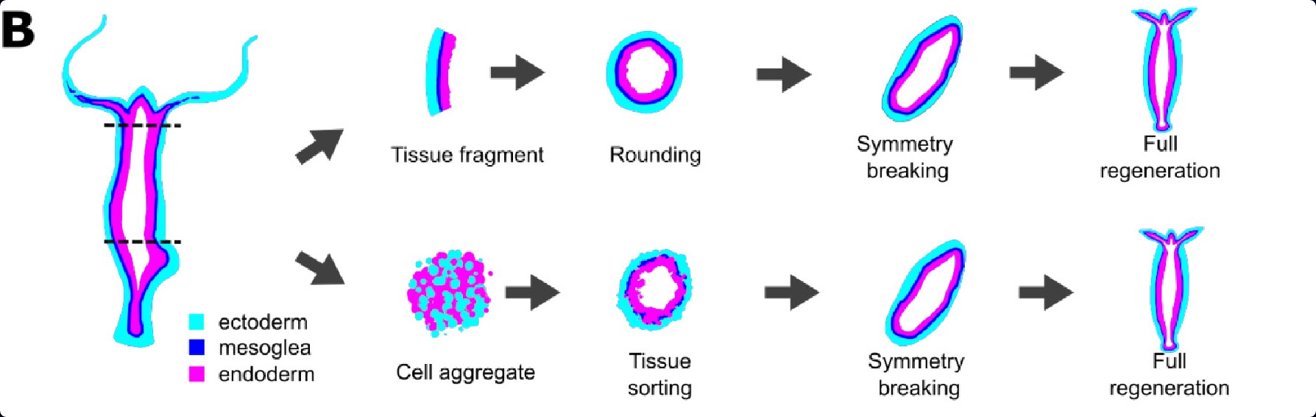
\includegraphics[
          width=0.94\textwidth,
          height=4.85cm,
          keepaspectratio
        ]{figures/hydra/hydra_regeneration_routes.png}
      };
    \end{tikzpicture}

    \vspace{0.04cm}

    {\color{HydraMuted}\fontsize{6}{7.2}\selectfont
      Wang, Bialas, Goel \& Collins,
      \textit{Integrative and Comparative Biology} 63 (2023), Fig.~1B.\par
    }
  \end{center}

  \vspace{0.12cm}

  \HydraTakeaway{
    Very different initial conditions pass through a similar spheroid stage
    before rebuilding a body axis
  }

\end{frame}


\begin{frame}{Symmetry breaks before a new head becomes visible}

  \begin{center}
    \begin{tikzpicture}
      \node[
        draw=HydraLine,
        rounded corners=4pt,
        inner sep=0.10cm
      ]{
        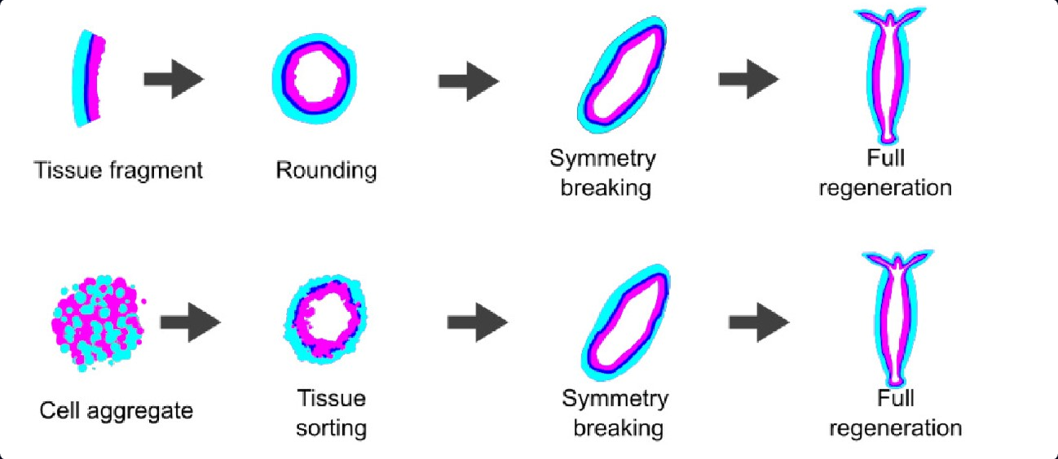
\includegraphics[
          width=0.80\textwidth,
          height=4.95cm,
          keepaspectratio
        ]{figures/hydra/hydra_symmetry_breaking_zoom.png}
      };
    \end{tikzpicture}

    \vspace{0.04cm}

    {\color{HydraMuted}\fontsize{6}{7.2}\selectfont
      Wang, Bialas, Goel \& Collins,
      \textit{Integrative and Comparative Biology} 63 (2023), Fig.~1B.\par
    }
  \end{center}

  \vspace{0.12cm}

  \HydraTakeaway{
    A local site acquires head-forming identity first; visible tentacles
    and the complete head--foot axis appear later
  }

\end{frame}

\HydraSubsection[
  Transplantation reveals that organizer activity depends on position and context.
]{Hydra grafting experiments}

\begin{frame}{A head graft can organize a second body axis}

  \begin{center}
    \begin{tikzpicture}
      \node[
        draw=HydraLine,
        rounded corners=4pt,
        inner sep=0.10cm
      ]{
        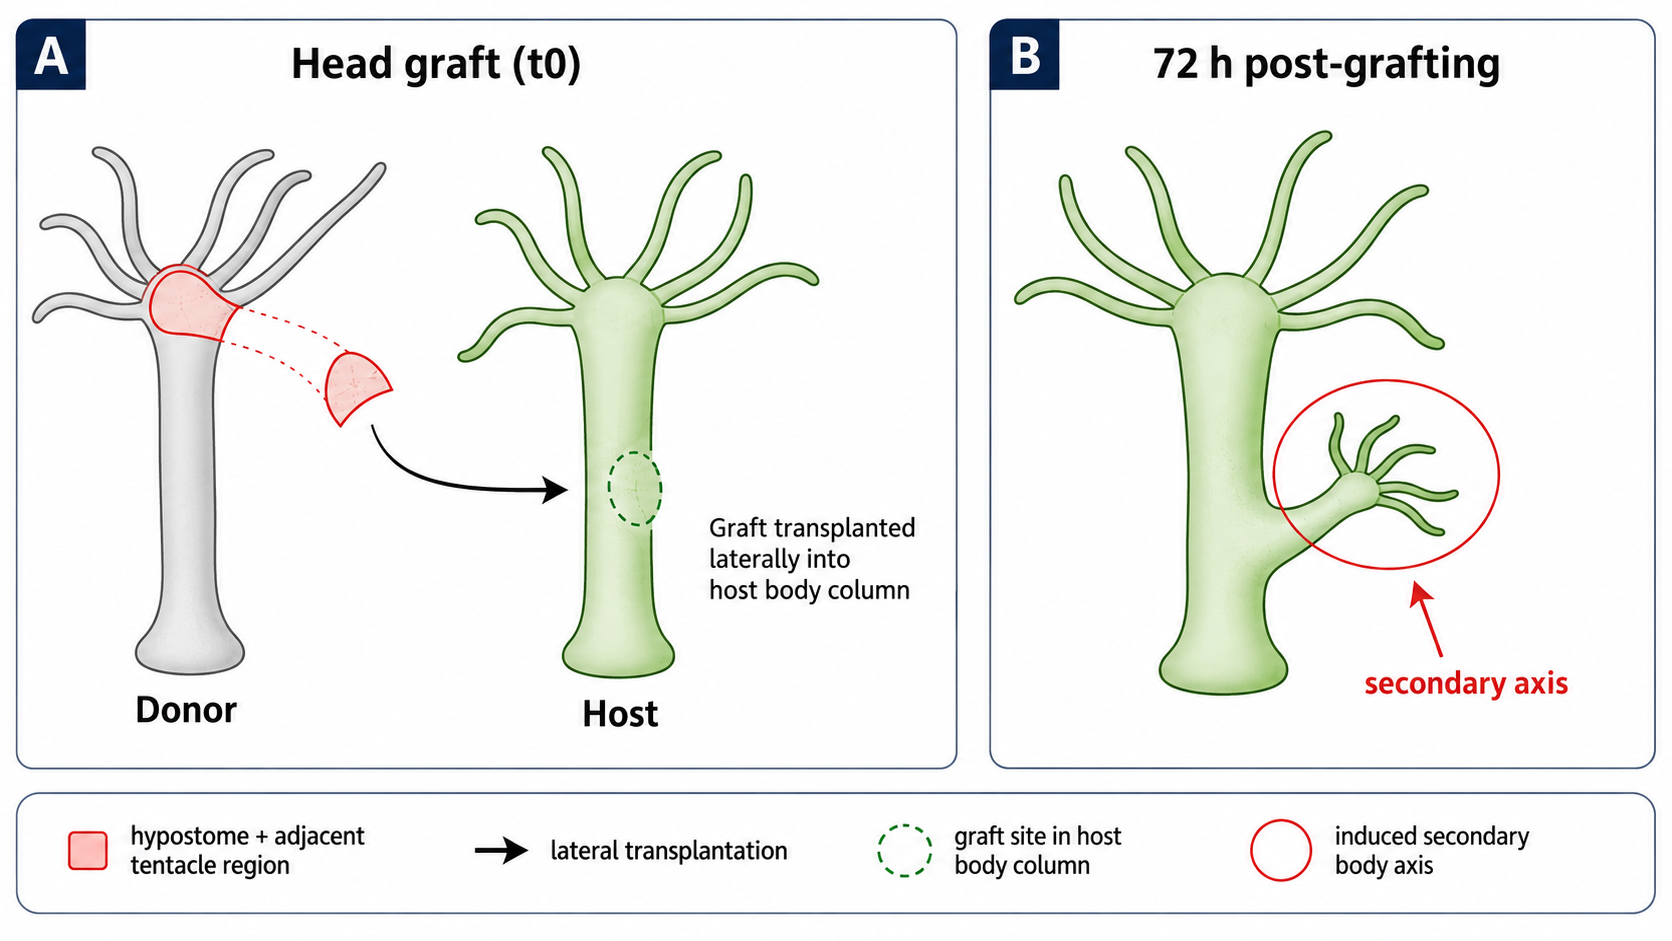
\includegraphics[
          width=0.92\textwidth,
          height=5.05cm,
          keepaspectratio
        ]{figures/hydra/a_clean_scientific_diagram_infographic_figure_wi_1.png}
      };
    \end{tikzpicture}

    \vspace{0.04cm}

    {\color{HydraMuted}\fontsize{6}{7.2}\selectfont
      Schematic based on the classic hypostome transplantation experiment
      of Browne (1909); see also Broun \& Bode (2002).\par
    }
  \end{center}

  \vspace{0.10cm}

  \HydraTakeaway{
    The graft does not simply grow into a second Hydra;
    it recruits a new body axis
  }

\end{frame}

\begin{frame}{Impact of the grafting position}

  \begin{center}
    \begin{tikzpicture}
      \node[
        draw=HydraLine,
        rounded corners=4pt,
        inner sep=0.10cm
      ]{
        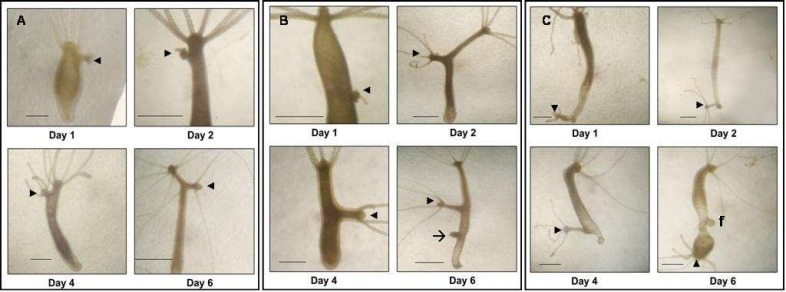
\includegraphics[
          width=0.92\textwidth,
          height=4.70cm,
          keepaspectratio
        ]{figures/hydra/grafting_timecourse.jpg}
      };
    \end{tikzpicture}

    \vspace{0.04cm}

    {\color{HydraMuted}\fontsize{6}{7.2}\selectfont
      Kadu, Ghaskadbi \& Ghaskadbi,
      \textit{Int. J. Mol. Cell. Med.}
      1 (2012).\par
    }
  \end{center}

  \vspace{0.10cm}

  \HydraTakeaway{
    The same graft can produce different outcomes depending on its position
  }

\end{frame}

\begin{frame}{Far from the host head: a complete second axis}

  \begin{columns}[T,onlytextwidth]

    \begin{column}{0.15\textwidth}
      \centering
      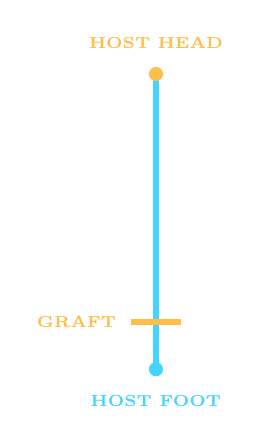
\begin{tikzpicture}[x=1cm,y=1cm]

        \draw[HydraCyan,line width=2pt] (0,0.35) -- (0,4.10);

        \fill[HydraGold] (0,4.10) circle[radius=0.09cm];
        \fill[HydraCyan] (0,0.35) circle[radius=0.09cm];

        \draw[HydraGold,line width=2pt]
          (-0.32,0.95) -- (0.32,0.95);

        \node[anchor=south,text=HydraGold,
          font=\bfseries\fontsize{5.8}{6.6}\selectfont]
          at (0,4.30) {HOST HEAD};

        \node[anchor=east,text=HydraGold,
          font=\bfseries\fontsize{5.8}{6.6}\selectfont]
          at (-0.38,0.95) {GRAFT};

        \node[anchor=north,text=HydraCyan,
          font=\bfseries\fontsize{5.8}{6.6}\selectfont]
          at (0,0.15) {HOST FOOT};

      \end{tikzpicture}

      \vspace{0.15cm}

      {\color{HydraMuted}\fontsize{6.2}{7.4}\selectfont
        lower host position\par}
    \end{column}

    \begin{column}{0.45\textwidth}
      \centering

      \begin{tikzpicture}
        \node[
          draw=HydraLine,
          rounded corners=4pt,
          inner sep=0.08cm
        ]{
          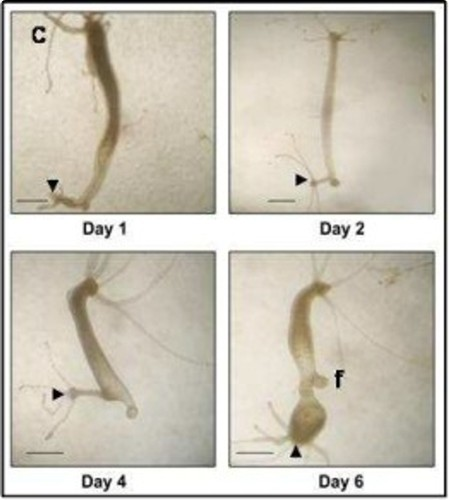
\includegraphics[
            width=\linewidth,
            height=4.65cm,
            keepaspectratio
          ]{figures/hydra/Bottom.jpg}
        };
      \end{tikzpicture}

      \vspace{0.04cm}

      {\color{HydraMuted}\fontsize{6}{7.2}\selectfont
        Kadu, Ghaskadbi \& Ghaskadbi,
        \textit{Int. J. Mol. Cell. Med.} 1 (2012), Fig.~2C.\par}
    \end{column}

    \begin{column}{0.34\textwidth}
      \vspace{0.5cm}
      \HydraPoint[HydraCyan]
        {A complete secondary axis}
        {The induced structure develops a foot, body column, hypostome and tentacles.}
      \vspace{0.7cm}
      \HydraPoint[HydraGold]
        {The strongest response}
        {Far from the host head, the same graft produces the longest and most complete secondary axis.}

    \end{column}

  \end{columns}

\end{frame}


\begin{frame}{Mid-body graft: an intermediate second axis}

  \begin{columns}[T,onlytextwidth]

    \begin{column}{0.15\textwidth}
      \centering
      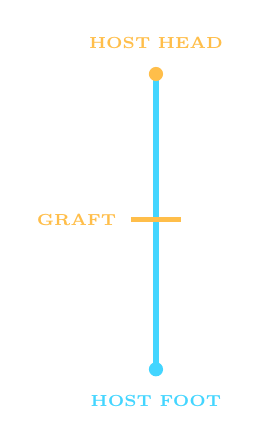
\begin{tikzpicture}[x=1cm,y=1cm]

        \draw[HydraCyan,line width=2pt] (0,0.35) -- (0,4.10);

        \fill[HydraGold] (0,4.10) circle[radius=0.09cm];
        \fill[HydraCyan] (0,0.35) circle[radius=0.09cm];

        \draw[HydraGold,line width=2pt]
          (-0.32,2.25) -- (0.32,2.25);

        \node[anchor=south,text=HydraGold,
          font=\bfseries\fontsize{5.8}{6.6}\selectfont]
          at (0,4.30) {HOST HEAD};

        \node[anchor=east,text=HydraGold,
          font=\bfseries\fontsize{5.8}{6.6}\selectfont]
          at (-0.38,2.25) {GRAFT};

        \node[anchor=north,text=HydraCyan,
          font=\bfseries\fontsize{5.8}{6.6}\selectfont]
          at (0,0.15) {HOST FOOT};

      \end{tikzpicture}

      \vspace{0.15cm}

      {\color{HydraMuted}\fontsize{6.2}{7.4}\selectfont
        middle host position\par}
    \end{column}

    \begin{column}{0.45\textwidth}
      \centering

      \begin{tikzpicture}
        \node[
          draw=HydraLine,
          rounded corners=4pt,
          inner sep=0.08cm
        ]{
          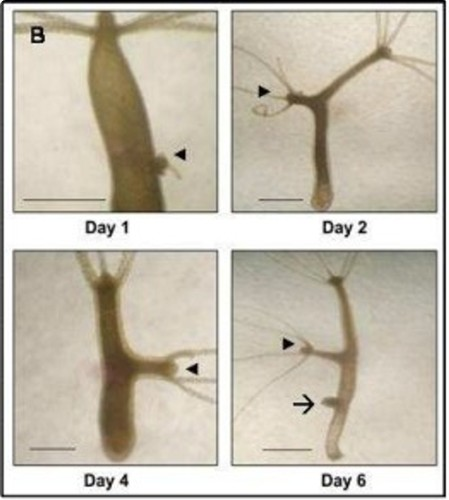
\includegraphics[
            width=\linewidth,
            height=4.65cm,
            keepaspectratio
          ]{figures/hydra/Middle.jpg}
        };
      \end{tikzpicture}

      \vspace{0.04cm}

      {\color{HydraMuted}\fontsize{6}{7.2}\selectfont
        Kadu, Ghaskadbi \& Ghaskadbi,
        \textit{Int. J. Mol. Cell. Med.} 1 (2012), Fig.~2B.\par}
    \end{column}

    \begin{column}{0.34\textwidth}
      \vspace{0.5cm}
      \HydraPoint[HydraCyan]
        {An intermediate secondary axis}
        {The induced axis grows substantially longer than after an upper-body graft.}
      \vspace{0.7cm}
      \HydraPoint[HydraGold]
        {Only position has changed}
        {The donor tissue is the same; moving the graft along the host axis changes the resulting morphology.}

    \end{column}

  \end{columns}

\end{frame}


\begin{frame}{Near the host head: only a short second axis}

  \begin{columns}[T,onlytextwidth]

    \begin{column}{0.15\textwidth}
      \centering
      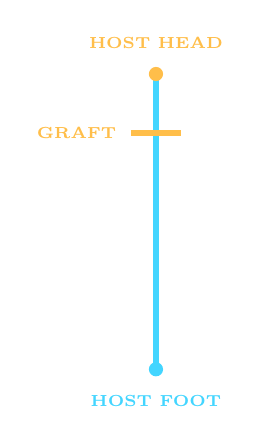
\begin{tikzpicture}[x=1cm,y=1cm]

        \draw[HydraCyan,line width=2pt] (0,0.35) -- (0,4.10);

        \fill[HydraGold] (0,4.10) circle[radius=0.09cm];
        \fill[HydraCyan] (0,0.35) circle[radius=0.09cm];

        \draw[HydraGold,line width=2pt]
          (-0.32,3.35) -- (0.32,3.35);

        \node[anchor=south,text=HydraGold,
          font=\bfseries\fontsize{5.8}{6.6}\selectfont]
          at (0,4.30) {HOST HEAD};

        \node[anchor=east,text=HydraGold,
          font=\bfseries\fontsize{5.8}{6.6}\selectfont]
          at (-0.38,3.35) {GRAFT};

        \node[anchor=north,text=HydraCyan,
          font=\bfseries\fontsize{5.8}{6.6}\selectfont]
          at (0,0.15) {HOST FOOT};

      \end{tikzpicture}

      \vspace{0.15cm}

      {\color{HydraMuted}\fontsize{6.2}{7.4}\selectfont
        upper host position\par}
    \end{column}

    \begin{column}{0.45\textwidth}
      \centering

      \begin{tikzpicture}
        \node[
          draw=HydraLine,
          rounded corners=4pt,
          inner sep=0.08cm
        ]{
          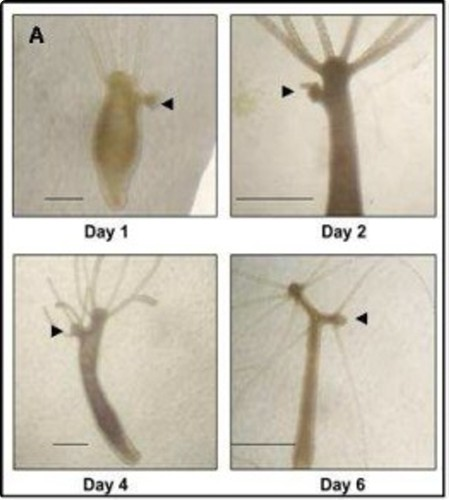
\includegraphics[
            width=\linewidth,
            height=4.65cm,
            keepaspectratio
          ]{figures/hydra/Top.jpg}
        };
      \end{tikzpicture}

      \vspace{0.04cm}

      {\color{HydraMuted}\fontsize{6}{7.2}\selectfont
        Kadu, Ghaskadbi \& Ghaskadbi,
        \textit{Int. J. Mol. Cell. Med.} 1 (2012), Fig.~2A.\par}
    \end{column}

    \begin{column}{0.34\textwidth}
      \vspace{0.5cm}
      \HydraPoint[HydraCyan]
        {A very short secondary axis}
        {The hypostome graft still induces a new head, but only a short body column develops.}
      \vspace{0.7cm}
      \HydraPoint[HydraGold]
        {Growth is strongly constrained}
        {Close to the host head, the induced axis remains small despite using the same organizer tissue.}

    \end{column}

  \end{columns}

\end{frame}


\begin{frame}{Multiple grafts can impose multiple axes}

  \begin{columns}[T,onlytextwidth]

    \begin{column}{0.47\textwidth}

      \vspace{0.9cm}

      \HydraPoint
        {Three grafts on one host}
          {A complete foot was grafted in the upper region, hypostome pieces were grafted in the middle and lower regions.}


      \vspace{0.3cm}

      \HydraPoint[HydraCyan]
        {Three secondary axes}
        {All three grafted regions produced an induction simultaneously.}

      \vspace{0.3cm}

      \HydraPoint
        {Organizer identity matters}
        {The axes induced by hypostome tissue were substantially longer than the axis induced by the foot graft.}


    \end{column}

    \begin{column}{0.49\textwidth}

      \centering

      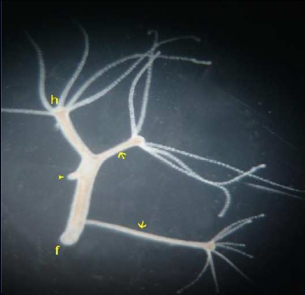
\includegraphics[
        width=\linewidth,
        height=5.55cm,
        keepaspectratio
      ]{figures/hydra/Multiple.png}

      \vspace{0.05cm}

      {\color{HydraMuted}\fontsize{6}{7.2}\selectfont
        Kadu, Ghaskadbi \& Ghaskadbi,
        \textit{Int. J. Mol. Cell. Med.} 1 (2012), Fig.~6.\par}

    \end{column}

  \end{columns}

  \vspace{0.20cm}

  \begin{center}
    \begin{minipage}{0.78\textwidth}
      \centering
      {\color{HydraGold}\bfseries\fontsize{9.0}{11.2}\selectfont
        Multiple local organizers can coexist and impose
        several body axes on the same tissue.\par}
    \end{minipage}
  \end{center}

\end{frame}





\begin{frame}{From experiments to a mathematical model}

  \vspace{0.20cm}
  \HydraProcess
    {regenerating tissue}
    {organizer selection}
    {one body axis}

  \vspace{0.40cm}

  \HydraProcess
    {ectopic organizer}
    {interaction with host}
    {secondary axis}

  \vspace{0.95cm}

  % ------------------------------------------------------------
  % Row 1
  % ------------------------------------------------------------
  \begin{columns}[T,onlytextwidth]

    \begin{column}{0.47\textwidth}
      \begin{minipage}[t][1.55cm][t]{\linewidth}
        \vspace{0pt}
        \HydraPoint[HydraGold]
          {Spontaneous pattern formation}
          {How can a localized organizer emerge from weakly patterned or nearly symmetric tissue?}
      \end{minipage}
    \end{column}

    \begin{column}{0.47\textwidth}
      \begin{minipage}[t][1.55cm][t]{\linewidth}
        \vspace{0pt}
        \HydraPoint[HydraGold]
          {Organizer induction}
          {Why can a transplanted organizer recruit host tissue and initiate a new axis?}
      \end{minipage}
    \end{column}

  \end{columns}

  \vspace{0.38cm}

  % ------------------------------------------------------------
  % Row 2
  % ------------------------------------------------------------
  \begin{columns}[T,onlytextwidth]

    \begin{column}{0.47\textwidth}
      \begin{minipage}[t][1.55cm][t]{\linewidth}
        \vspace{0pt}
        \HydraPoint[HydraGold]
          {Competition and uniqueness}
          {Why does normal regeneration usually select one head, while several grafts can sustain several axes?}
      \end{minipage}
    \end{column}

    \begin{column}{0.47\textwidth}
      \begin{minipage}[t][1.55cm][t]{\linewidth}
        \vspace{0pt}
        \HydraPoint[HydraGold]
      {Context dependence}
      {Why does the same hypostome graft produce different secondary axes at different positions in the host?}
      \end{minipage}
    \end{column}

  \end{columns}

  \vfill

  % \HydraTakeaway{
  %   A mathematical model should capture both self-organization
  %   and the response to an imposed organizer.
  % }

\end{frame}
\HydraSection[
  focus x=0.62,
  focus y=0.44,
  radius=0.12,
  zoom=1.90
]{Reaction--diffusion approach}

\HydraSubsection[
  Chemical signals provide a natural mechanism for spatial organization.
]{Chemical  \mbox{patterning}}

\begin{frame}{Could chemical signals determine where a head forms?}

  \HydraTextImage[5.65cm]{
    \vspace{0.5cm}
    \HydraPoint[HydraGold]
      {Cells communicate through chemical signals}
      {Signaling molecules can be produced, transformed and removed by cells.}

    \vspace{0.18cm}

    \HydraPoint[HydraCyan]
      {Concentrations can vary in space}
      {Different regions of the tissue may therefore experience different levels of the same signal.}

    \vspace{0.18cm}

    \HydraPoint[HydraGold]
      {A local maximum can select a site}
      {A sufficiently high concentration may trigger head-forming activity in one particular region.}

    \vspace{0.18cm}

    \HydraPoint[HydraCyan]
      {Chemistry can position the organizer}
      {{The location of head formation becomes a question of how a spatial concentration pattern arises.}}

  }
  {figures/B_reaction_diffusion/Concentration.png}
  {}

  \vspace{0.10cm}

  % \HydraTakeaway{
  %   One possible mechanism is that a spatial pattern of chemical signals
  %   selects the position of the head organizer.
  % }

\end{frame}


\begin{frame}{Reactions change signals, diffusion moves them}

  \vspace{0.30cm}

  \begin{columns}[T,onlytextwidth]

    \begin{column}{0.46\textwidth}

      {\color{HydraGold}\bfseries
       \fontsize{11.5}{13.5}\selectfont
       REACTION\par}

      \vspace{0.35cm}

      \HydraPoint[HydraGold]
        {Local chemical change}
        {Cells can produce, remove or transform signaling molecules.}

      \vspace{0.25cm}

      \HydraPoint[HydraGold]
        {Local feedback}
        {The production of a signal may depend on the concentrations already present in the same region.}

    \end{column}

    \begin{column}{0.46\textwidth}

      {\color{HydraCyan}\bfseries
       \fontsize{11.5}{13.5}\selectfont
       DIFFUSION\par}

      \vspace{0.35cm}

      \HydraPoint[HydraCyan]
        {Spatial redistribution}
        {Signaling molecules spread from regions of higher concentration toward regions of lower concentration.}

      \vspace{0.25cm}

      \HydraPoint[HydraCyan]
        {Communication across tissue}
        {Diffusion couples nearby regions, allowing a local chemical change to influence its surroundings.}

    \end{column}

  \end{columns}

  \vfill

  % \HydraTakeaway{
  %   Pattern formation becomes possible when local chemical feedback
  %   is coupled to spatial communication.
  % }

\end{frame}




\begin{frame}{Mechanism of chemical pattern formation}

  \vspace{0.12cm}

  \begin{columns}[c,onlytextwidth]

    % ----------------------------------------------------------
    % Turing + original paper
    % ----------------------------------------------------------
    \begin{column}{0.29\textwidth}
      \centering

      \begin{minipage}{0.72\linewidth}
        \centering
        \includegraphics[
          width=\linewidth,
          height=2.35cm,
          keepaspectratio
        ]{figures/common/Alan_Turing_(1951).jpg}
      \end{minipage}

      \vspace{0.08cm}

      {\color{HydraGold}\bfseries
       \fontsize{19}{22}\selectfont 1952\par}

      {\color{HydraWhite}\bfseries
       \fontsize{9.5}{11}\selectfont Alan Turing\par}

      \vspace{0.18cm}

      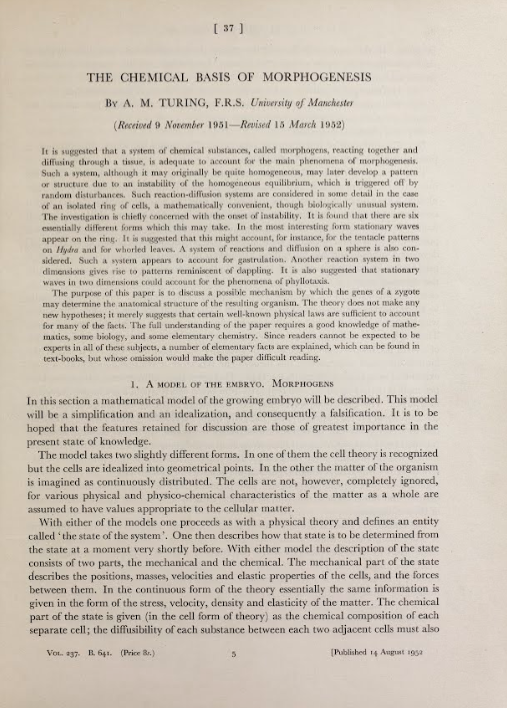
\includegraphics[
        width=0.66\linewidth,
        height=2.15cm,
        keepaspectratio
      ]{figures/B_reaction_diffusion/TuringPaper.png}

    \end{column}

    % ----------------------------------------------------------
    % Main message
    % ----------------------------------------------------------
    \begin{column}{0.65\textwidth}

      \HydraPoint[HydraGold]
        {A homogeneous tissue need not stay homogeneous}
        {Chemical substances can react and diffuse through tissue, allowing spatial structure to emerge from small perturbations.}

      \vspace{0.18cm}

      \HydraPoint[HydraCyan]
        {Diffusion becomes part of the mechanism}
        {Spatial transport is not merely smoothing: together with reactions it can participate in pattern formation.}

      \vspace{0.18cm}

      \HydraPoint
        {Hydra was already on the list}
        {Turing explicitly mentioned stationary patterns as a possible explanation for tentacle organization in Hydra.}

    \end{column}

  \end{columns}

  \vspace{0.15cm}

  \HydraTakeaway{
    Reaction and diffusion can, in principle, turn an almost homogeneous state into spatial structure
  }
  
  % \vspace{0.40cm}
  % \source{
    % A.~M. Turing, \textit{Phil. Trans. R. Soc. B} 237 (1952), 37--72.
    % Portrait: Elliott \& Fry, 1951, Wikimedia Commons.
  % }

\end{frame}

\begin{frame}{Gierer and Meinhardt propose a model}

  \vspace{0.15cm}

  \begin{columns}[T,onlytextwidth]

    % ----------------------------------------------------------
    % Portraits
    % ----------------------------------------------------------
    \begin{column}{0.30\textwidth}
      \centering

      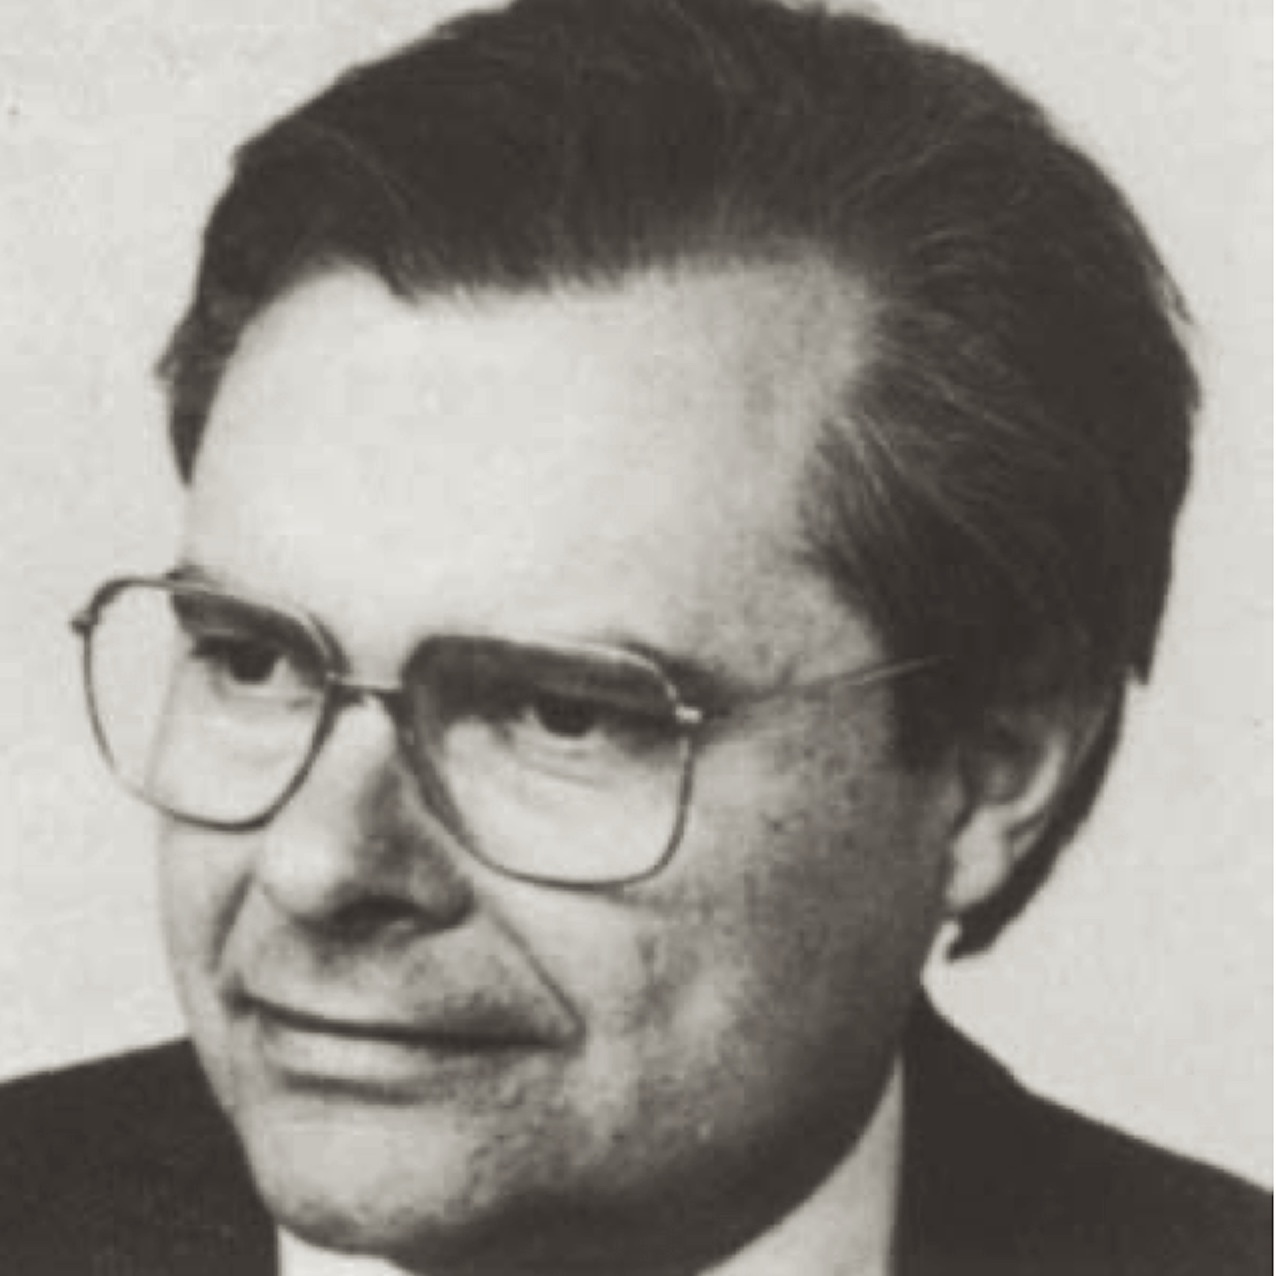
\includegraphics[
        width=0.72\linewidth,
        height=2.25cm,
        keepaspectratio
      ]{figures/B_reaction_diffusion/Alfred_Gierer.jpg}

      \vspace{0.07cm}

      {\color{HydraWhite}\bfseries\fontsize{8.5}{10}\selectfont
        Alfred Gierer\par}

      \vspace{0.28cm}

      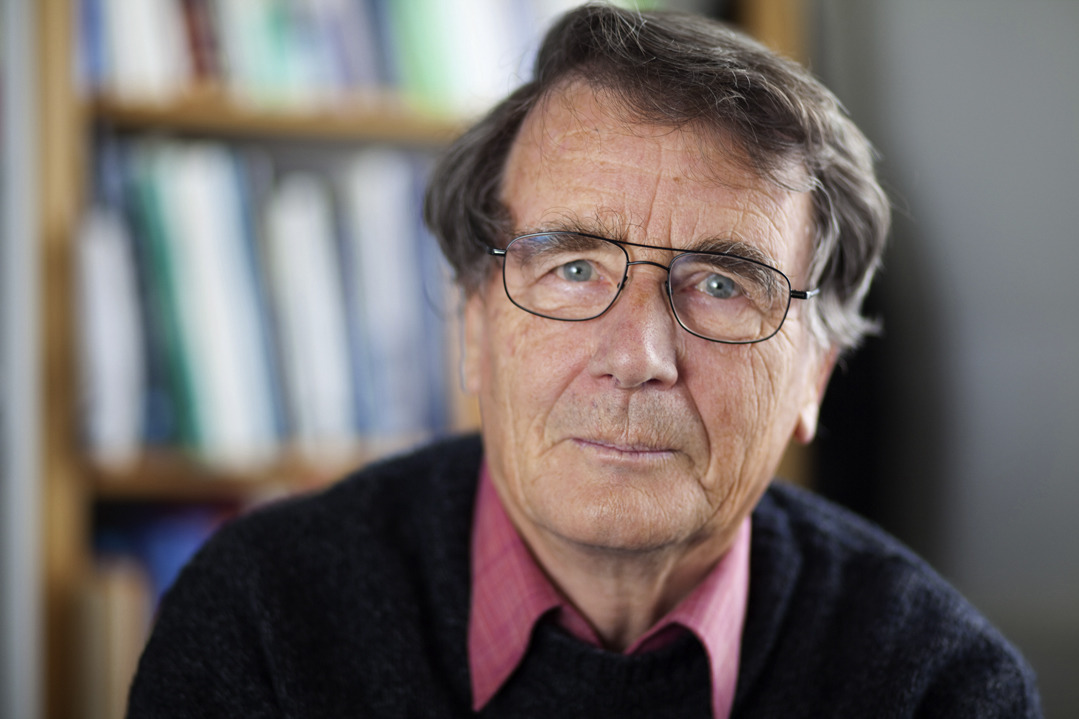
\includegraphics[
        width=0.72\linewidth,
        height=2.25cm,
        keepaspectratio
      ]{figures/B_reaction_diffusion/Hans_Meinhardt.jpg}

      \vspace{0.07cm}

      {\color{HydraWhite}\bfseries\fontsize{8.5}{10}\selectfont
        Hans Meinhardt\par}

    \end{column}

    % ----------------------------------------------------------
    % Paper + mechanism
    % ----------------------------------------------------------
    \begin{column}{0.64\textwidth}

      {\color{HydraGold}\bfseries\fontsize{9}{10.5}\selectfont
        A. GIERER \& H. MEINHARDT   /   1972 \par}

      \vspace{0.08cm}

      {\color{HydraWhite}\bfseries\fontsize{15}{18}\selectfont
        \textit{A Theory of Biological Pattern Formation}\par}

      \vspace{0.18cm}

      {\color{HydraMuted}\fontsize{8.2}{10.5}\selectfont
        A mechanism for generating spatial organization
        in an initially almost homogeneous tissue.\par}

      \vspace{0.48cm}

      \HydraPoint[HydraGold]
        {Local self-activation}
        {A small local excess reinforces itself and can develop into a localized organizing region.}

      \vspace{0.30cm}

      \HydraPoint[HydraCyan]
        {Long-range inhibition}
        {The activated region generates an inhibitory effect that acts over a larger spatial range.}

    \end{column}

  \end{columns}

  \source{
    Gierer \& Meinhardt,
    \textit{Kybernetik} 12 (1972), 30--39.
  }

\end{frame}

\begin{frame}{The activator--inhibitor idea}

  \begin{center}
    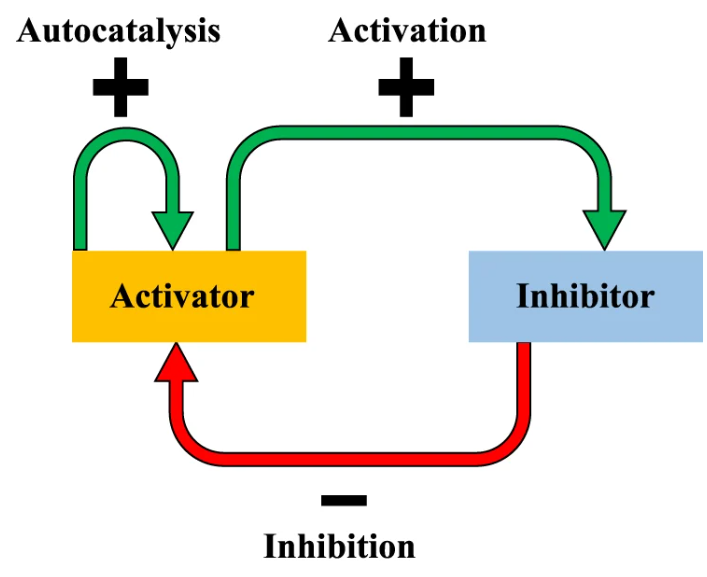
\includegraphics[
      width=0.85\textwidth,
      height=5.5cm,
      keepaspectratio
    ]{figures/B_reaction_diffusion/ActivatorInhibitor.png}

    % \vspace{0.05cm}

    % {\color{HydraMuted}\fontsize{6}{7.2}\selectfont
      % Schematic illustration of local activation and long-range inhibition.\par}
  \end{center}

  \vspace{0.08cm}

  \begin{columns}[T,onlytextwidth]

    \begin{column}{0.47\textwidth}
      \HydraPoint[HydraGold]
        {Activator}
        {Enhances its own production and promotes local organizer formation. Its effect remains relatively localized.}
    \end{column}

    \begin{column}{0.47\textwidth}
      \HydraPoint[HydraCyan]
        {Inhibitor}
        {Is produced by activated regions, suppresses further activation and acts over a longer spatial range.}
    \end{column}

  \end{columns}

\end{frame}



\begin{frame}{The Gierer--Meinhardt model}

  \vspace{-0.50cm}

  \begin{columns}[c,onlytextwidth]

    % ----------------------------------------------------------
    % Equations
    % ----------------------------------------------------------
    \begin{column}{0.65\textwidth}

      {\color{HydraWhite}\fontsize{12.5}{17}\selectfont
      \begin{align*}
        \partial_t u
        &=
        \underbrace{
          D_u\Delta u
        }_{\color{HydraCyan}\text{diffusion}}
        \quad+\quad
        \underbrace{
          \frac{a u^2}{K+v}-\mu_u u
        }_{\color{HydraGold}\text{reaction}}
        \\[0.75cm]
        \partial_t v
        &=
        \underbrace{
          D_v\Delta v
        }_{\color{HydraCyan}\text{diffusion}}
        \quad+\quad
        \underbrace{
          b u^2-\mu_v v
        }_{\color{HydraGold}\text{reaction}}
      \end{align*}
      }

    \end{column}

    % ----------------------------------------------------------
    % Variables
    % ----------------------------------------------------------
    \begin{column}{0.30\textwidth}
      \vspace{0.10cm}

      \HydraPoint[HydraGold]
        {$u$: activator}
        {Promotes its own production and initiates local organizer activity}

      \vspace{0.55cm}

      \HydraPoint[HydraCyan]
        {$v$: inhibitor}
        {Produced by the activator and suppresses its production}

    \end{column}

  \end{columns}

  \vspace{0.25cm}

  % ----------------------------------------------------------
  % Parameters
  % ----------------------------------------------------------
  {\color{HydraWhite}\fontsize{8.8}{11.3}\selectfont

  \begin{columns}[t,onlytextwidth]

    \begin{column}{0.47\textwidth}

      \textcolor{HydraCyan}{$D_u,\;D_v$}
      \quad diffusion rates, typically $D_v>D_u$

      \vspace{0.18cm}

      \textcolor{HydraGold}{$a$}
      \quad strength of activator self-amplification

      \vspace{0.18cm}

      \textcolor{HydraGold}{$b$}
      \quad strength of inhibitor production

    \end{column}

    \begin{column}{0.47\textwidth}

      \textcolor{HydraGold}{$K$}
      \quad scale of inhibition by $v$

      \vspace{0.18cm}

      \textcolor{HydraGold}{$\mu_u$}
      \quad activator degradation rate

      \vspace{0.18cm}

      \textcolor{HydraGold}{$\mu_v$}
      \quad inhibitor degradation rate

    \end{column}

  \end{columns}
  }

\end{frame}

\begin{frame}{A general reaction--diffusion system}

  \vspace{0.10cm}

  \begin{columns}[c,onlytextwidth]

    \begin{column}{0.65\textwidth}
      {\color{HydraWhite}\fontsize{12.5}{17}\selectfont
      \begin{align*}
        \partial_t u
        &=
        \underbrace{D_u\Delta u}_{\color{HydraCyan}\text{diffusion}}
        \quad+\quad
        \underbrace{f(u,v)}_{\color{HydraGold}\text{reaction}},
        \\[0.75cm]
        \partial_t v
        &=
        \underbrace{D_v\Delta v}_{\color{HydraCyan}\text{diffusion}}
        \quad+\quad
        \underbrace{g(u,v)}_{\color{HydraGold}\text{reaction}}.
      \end{align*}
      }
    \end{column}

    \begin{column}{0.30\textwidth}
      \HydraPoint[HydraGold]
        {$u$ and $v$}
        {Concentrations of two interacting chemical signals.}

      \vspace{0.38cm}

      \HydraPoint[HydraGold]
        {$f$ and $g$}
        {Possibly nonlinear local production, removal and interaction terms.}
    \end{column}

  \end{columns}

  \vfill

  \HydraTakeaway{
    We begin by deriving the spatial transport term
  }

\end{frame}

\HydraSubsection[
  \mbox{Diffusion redistributes signals} \mbox{through space and smooths} \mbox{concentration differences}
]{Diffusion}





\begin{frame}{Diffusion begins with a local balance}

  \vspace{0.25cm}

  \begin{columns}[c,onlytextwidth]

    \begin{column}{0.32\textwidth}
      \HydraPoint[HydraCyan]
        {Concentration}
        {$u(x,t)$ measures the amount of a substance per unit length at point $x$.}

      \vspace{0.38cm}

      \HydraPoint[HydraGold]
        {Control volume}
        {We track the substance inside a short interval of length $\Delta x$.}
    \end{column}

    \begin{column}{0.64\textwidth}
      \centering
      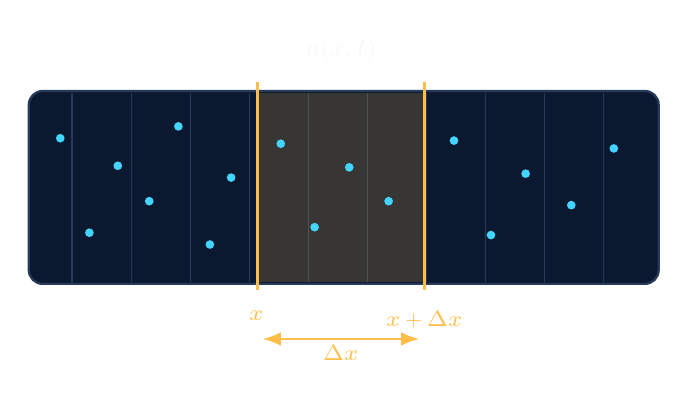
\begin{tikzpicture}[x=1cm,y=1cm]
        \fill[HydraPanel,rounded corners=5pt]
          (0.15,0.70) rectangle (8.15,3.15);
        \draw[HydraLine,line width=0.8pt,rounded corners=5pt]
          (0.15,0.70) rectangle (8.15,3.15);

        \foreach \x in {0.70,1.45,2.20,2.95,3.70,4.45,5.20,5.95,6.70,7.45}{
          \draw[HydraLine,line width=0.45pt]
            (\x,0.72) -- (\x,3.13);
        }

        \fill[HydraGold,opacity=0.18]
          (3.05,0.72) rectangle (5.18,3.13);
        \draw[HydraGold,line width=1.15pt]
          (3.05,0.62) -- (3.05,3.26);
        \draw[HydraGold,line width=1.15pt]
          (5.18,0.62) -- (5.18,3.26);

        \foreach \px/\py in {0.55/2.55,0.92/1.35,1.28/2.20,1.68/1.75,
          2.05/2.70,2.45/1.20,2.72/2.05,3.35/2.48,
          3.78/1.42,4.22/2.18,4.72/1.75,5.55/2.52,
          6.02/1.32,6.46/2.10,7.04/1.70,7.58/2.42}{
          \fill[HydraCyan] (\px,\py) circle[radius=0.055cm];
        }

        \node[anchor=south,text=HydraWhite,
          font=\bfseries\fontsize{9.5}{11}\selectfont]
          at (4.12,3.38) {$u(x,t)$};
        \node[anchor=north,text=HydraGold,
          font=\bfseries\fontsize{8}{9.5}\selectfont]
          at (3.05,0.48) {$x$};
        \node[anchor=north,text=HydraGold,
          font=\bfseries\fontsize{8}{9.5}\selectfont]
          at (5.18,0.48) {$x+\Delta x$};

        \draw[<->,>=Latex,HydraGold,line width=0.8pt]
          (3.12,0.0) -- (5.11,0.0);
        \node[text=HydraGold,font=\fontsize{8}{9.5}\selectfont]
          at (4.12,-0.18) {$\Delta x$};
      \end{tikzpicture}

      \vspace{0.15cm}

      {\color{HydraWhite}\fontsize{11.5}{14}\selectfont
        \[
          \text{amount in the interval}
          \;\approx\;
          u(x,t)\,\Delta x
        \]
      }
    \end{column}

  \end{columns}

\end{frame}


\begin{frame}{Boundary flux}

  \vspace{0.12cm}

  \begin{columns}[c,onlytextwidth]

    \begin{column}{0.74\textwidth}
      \centering
      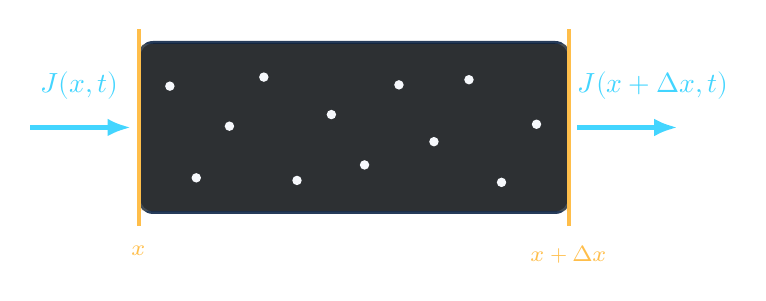
\begin{tikzpicture}[x=0.78cm,y=0.82cm]
        \fill[HydraPanel,rounded corners=5pt]
          (2.15,1.18) rectangle (9.15,3.82);
        \draw[HydraLine,line width=0.9pt,rounded corners=5pt]
          (2.15,1.18) rectangle (9.15,3.82);
        \fill[HydraGold,opacity=0.14]
          (2.18,1.21) rectangle (9.12,3.79);

        \draw[HydraGold,line width=1.2pt]
          (2.15,0.98) -- (2.15,4.02);
        \draw[HydraGold,line width=1.2pt]
          (9.15,0.98) -- (9.15,4.02);

        \draw[-{Latex[length=3mm]},HydraCyan,line width=2.0pt]
          (0.38,2.50) -- (2.02,2.50);
        \draw[-{Latex[length=3mm]},HydraCyan,line width=2.0pt]
          (9.28,2.50) -- (10.92,2.50);

        \node[anchor=south,text=HydraCyan,
          font=\bfseries\fontsize{10}{11.5}\selectfont]
          at (1.18,2.78) {$J(x,t)$};
        \node[anchor=south,text=HydraCyan,
          font=\bfseries\fontsize{10}{11.5}\selectfont]
          at (10.52,2.78) {$J(x+\Delta x,t)$};

        \foreach \px/\py in {2.65/3.14,3.08/1.72,3.62/2.52,4.18/3.28,
          4.72/1.68,5.28/2.70,5.82/1.92,6.38/3.16,
          6.95/2.28,7.52/3.24,8.05/1.65,8.62/2.55}{
          \fill[HydraWhite] (\px,\py) circle[radius=0.06cm];
        }

        \node[anchor=north,text=HydraGold,
          font=\bfseries\fontsize{8}{9.5}\selectfont]
          at (2.15,0.82) {$x$};
        \node[anchor=north,text=HydraGold,
          font=\bfseries\fontsize{8}{9.5}\selectfont]
          at (9.15,0.82) {$x+\Delta x$};
      \end{tikzpicture}

      \vspace{0.10cm}

      {\color{HydraMuted}\fontsize{8.4}{10}\selectfont
        \textcolor{HydraCyan}{\bfseries Flux $J$:}
        amount of substance crossing a boundary.
      \par}

      \vspace{0.12cm}

      {\color{HydraWhite}\fontsize{11.2}{14.5}\selectfont
      \[
        \frac{
          u(x,t+\Delta t)\,\Delta x-u(x,t)\,\Delta x
        }{\Delta t}
        =
        \textcolor{HydraCyan}{J(x,t)}
        -
        \textcolor{HydraCyan}{J(x+\Delta x,t)}
      \]
      }
    \end{column}

    \begin{column}{0.22\textwidth}
      {\color{HydraMuted}\fontsize{7.1}{8.7}\selectfont
        \textcolor{HydraWhite}{$J(x,t)>J(x+\Delta x,t)$}
        \par
        \vspace{0.04cm}
        amount increases

        \vspace{0.42cm}

        \textcolor{HydraWhite}{$J(x,t)=J(x+\Delta x,t)$}
        \par
        \vspace{0.04cm}
        amount stays constant

        \vspace{0.42cm}

        \textcolor{HydraWhite}{$J(x,t)<J(x+\Delta x,t)$}
        \par
        \vspace{0.04cm}
        amount decreases
      }
    \end{column}

  \end{columns}

  \vfill

  \HydraTakeaway{
    Only a difference between the boundary fluxes changes the amount inside
  }

\end{frame}


\begin{frame}{The local conservation law}

  \vspace{0.08cm}

  \begin{center}
    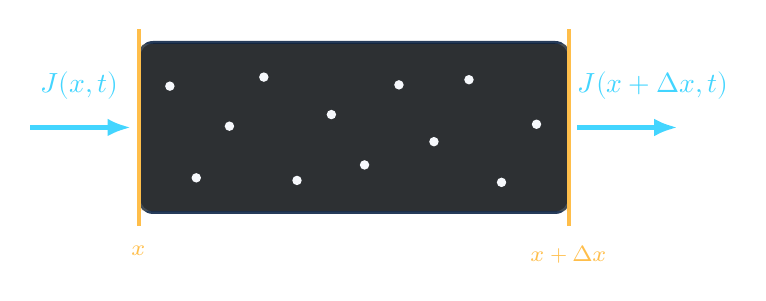
\begin{tikzpicture}[x=0.78cm,y=0.82cm]
      \fill[HydraPanel,rounded corners=5pt]
        (2.15,1.18) rectangle (9.15,3.82);
      \draw[HydraLine,line width=0.9pt,rounded corners=5pt]
        (2.15,1.18) rectangle (9.15,3.82);
      \fill[HydraGold,opacity=0.14]
        (2.18,1.21) rectangle (9.12,3.79);

      \draw[HydraGold,line width=1.2pt]
        (2.15,0.98) -- (2.15,4.02);
      \draw[HydraGold,line width=1.2pt]
        (9.15,0.98) -- (9.15,4.02);

      \draw[-{Latex[length=3mm]},HydraCyan,line width=2.0pt]
        (0.38,2.50) -- (2.02,2.50);
      \draw[-{Latex[length=3mm]},HydraCyan,line width=2.0pt]
        (9.28,2.50) -- (10.92,2.50);

      \node[anchor=south,text=HydraCyan,
        font=\bfseries\fontsize{10}{11.5}\selectfont]
        at (1.18,2.78) {$J(x,t)$};
      \node[anchor=south,text=HydraCyan,
        font=\bfseries\fontsize{10}{11.5}\selectfont]
        at (10.52,2.78) {$J(x+\Delta x,t)$};

      \foreach \px/\py in {2.65/3.14,3.08/1.72,3.62/2.52,4.18/3.28,
        4.72/1.68,5.28/2.70,5.82/1.92,6.38/3.16,
        6.95/2.28,7.52/3.24,8.05/1.65,8.62/2.55}{
        \fill[HydraWhite] (\px,\py) circle[radius=0.06cm];
      }

      \node[anchor=north,text=HydraGold,
        font=\bfseries\fontsize{8}{9.5}\selectfont]
        at (2.15,0.82) {$x$};
      \node[anchor=north,text=HydraGold,
        font=\bfseries\fontsize{8}{9.5}\selectfont]
        at (9.15,0.82) {$x+\Delta x$};
    \end{tikzpicture}
  \end{center}

  \vspace{-0.58cm}

  \begin{center}
    {\color{HydraWhite}\fontsize{11.5}{15}\selectfont
    \[
      \frac{u(x,t+\Delta t)-u(x,t)}{\Delta t}
      =
      -\frac{
        \textcolor{HydraCyan}{J(x+\Delta x,t)}
        -\textcolor{HydraCyan}{J(x,t)}
      }{\Delta x}
    \]
    }

    \vspace{-0.10cm}

\begin{center}
  {\color{HydraCyan}\fontsize{18}{18}\selectfont
    $\Downarrow$
    \rlap{%
      \hspace{0.25cm}%
      {\fontsize{9.5}{11.5}\selectfont
        $\Delta t,\Delta x\longrightarrow0$%
      }%
    }
  \par}
\end{center}

    \vspace{-0.72cm}

    {\color{HydraWhite}\bfseries\fontsize{17}{21}\selectfont
    \[
      \boxed{\partial_tu=-\partial_xJ}
    \]
    }
  \end{center}

\end{frame}


\begin{frame}{Fick's law of diffusion}

  \vspace{0.04cm}

  \begin{columns}[c,onlytextwidth]

    \begin{column}{0.27\textwidth}
      \centering

      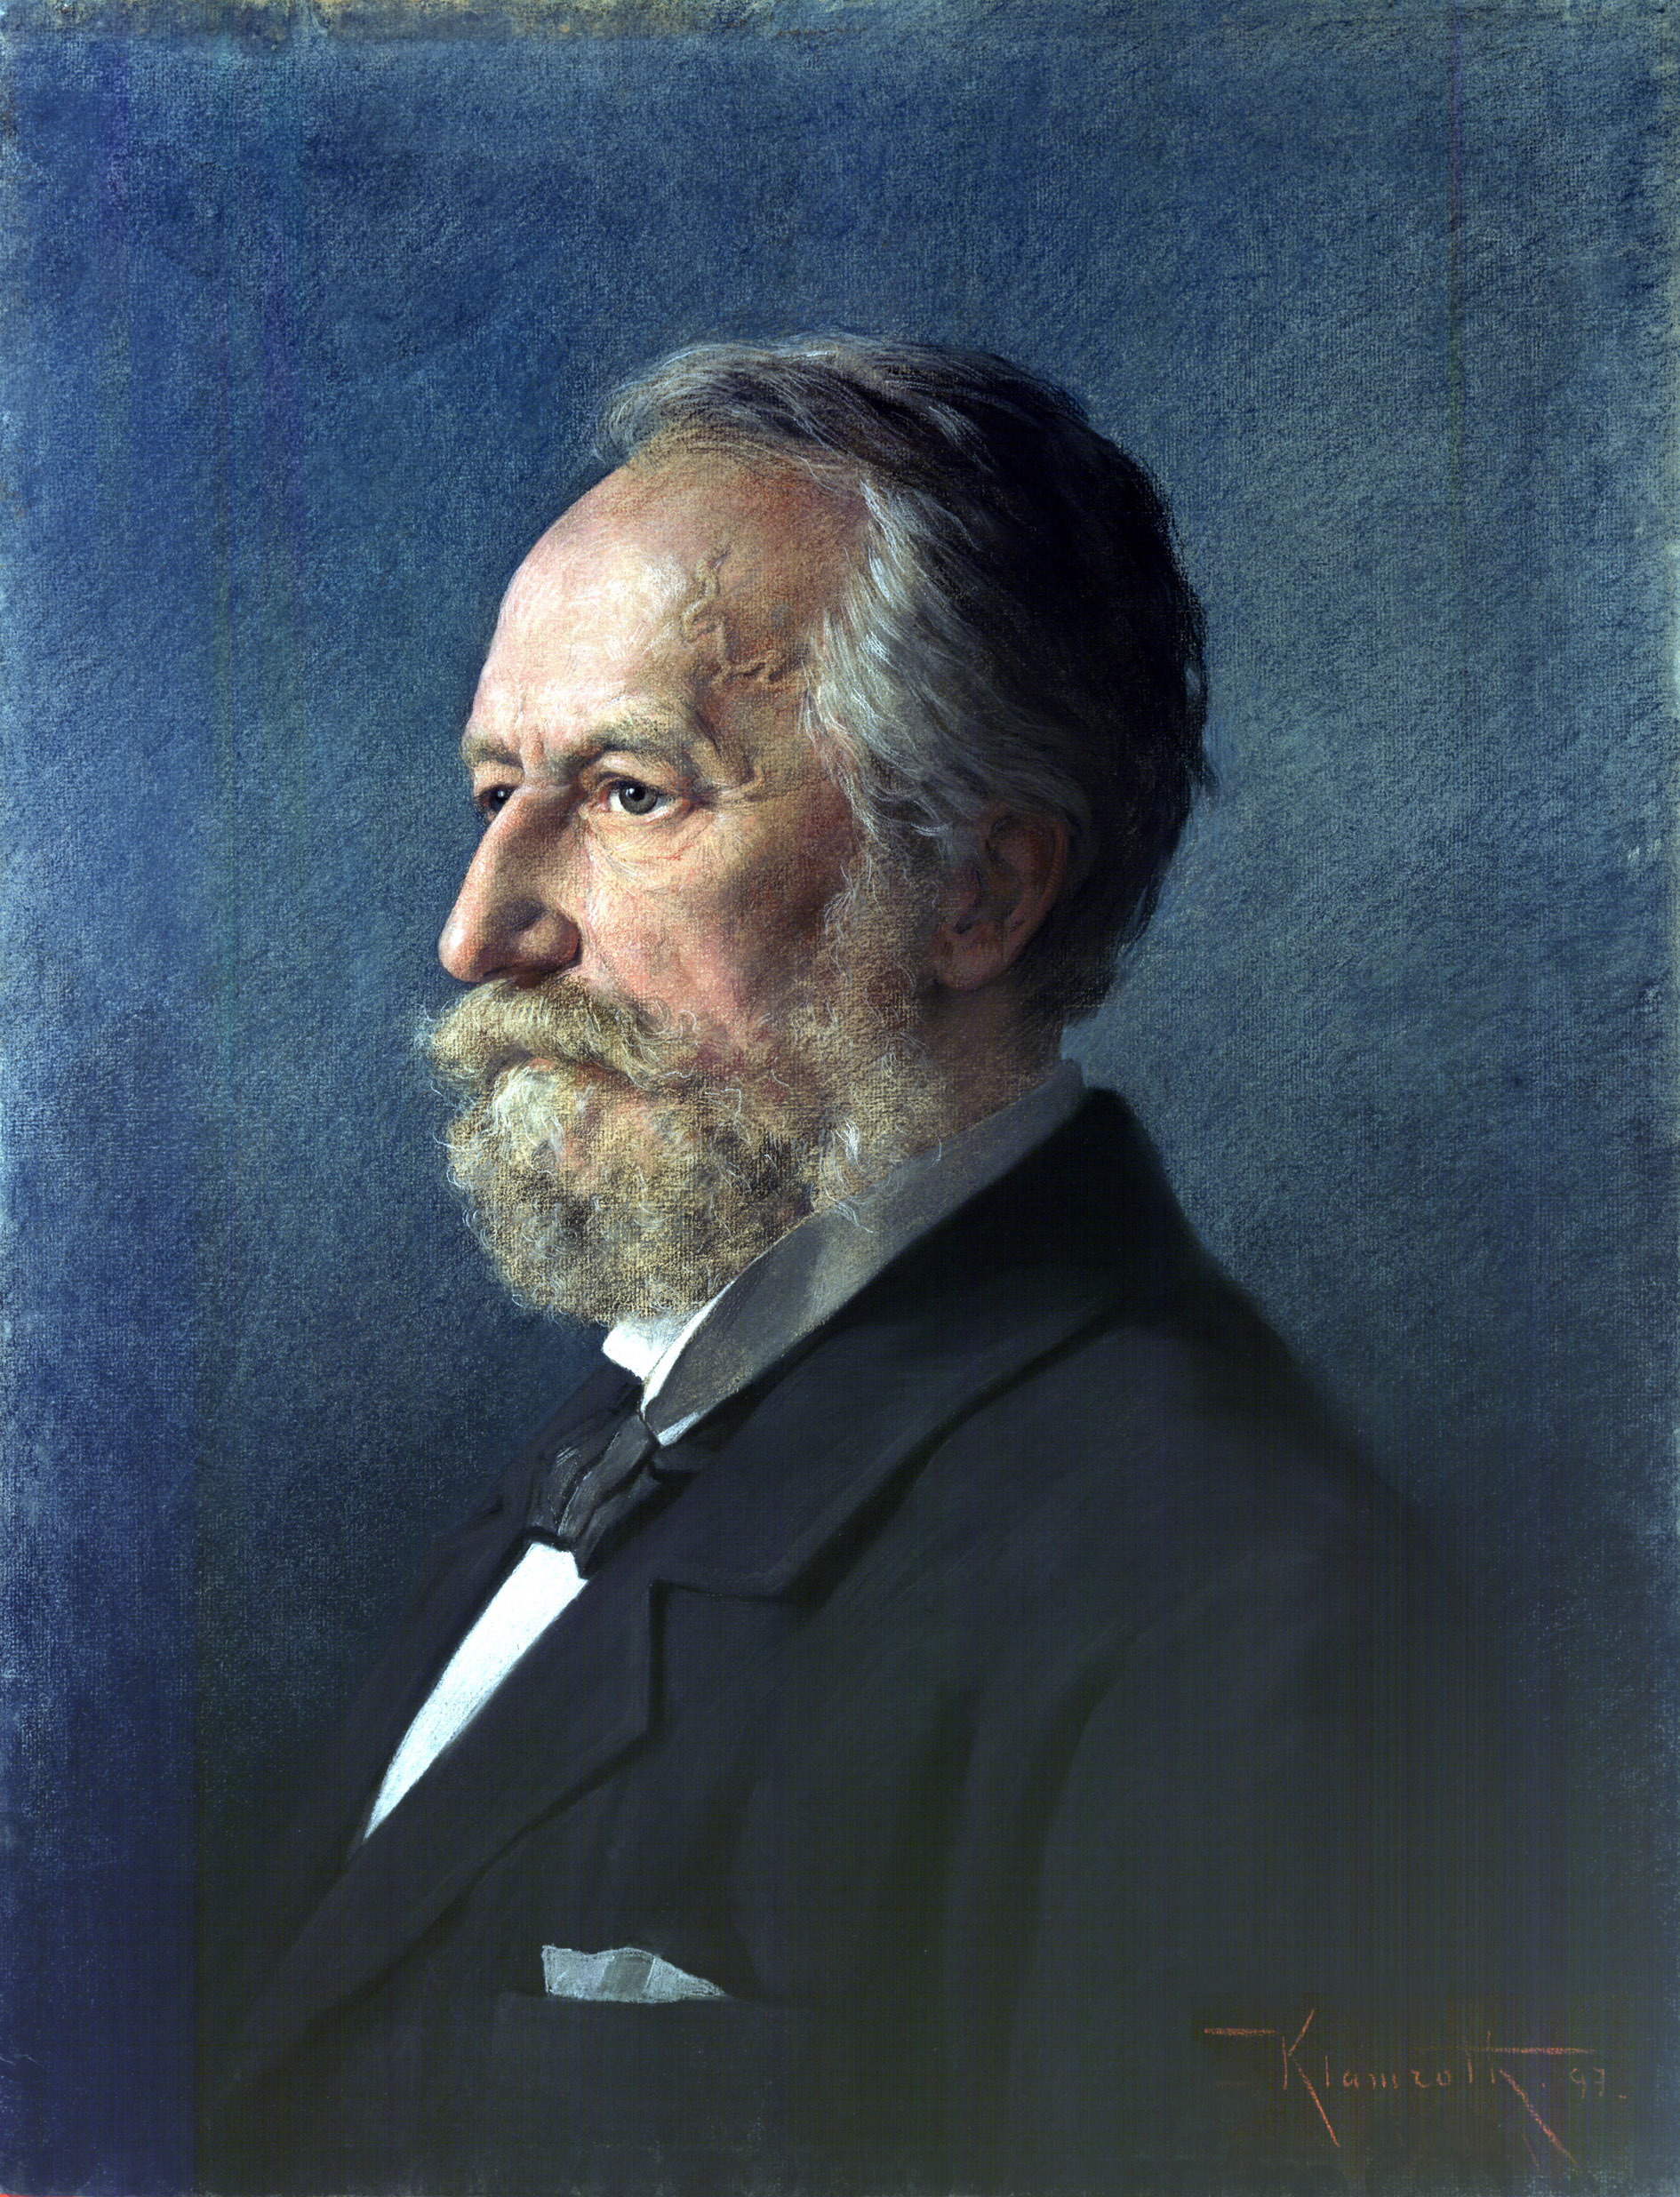
\includegraphics[
        width=0.70\linewidth,
        height=2.65cm,
        keepaspectratio
      ]{figures/B_reaction_diffusion/Adolf_Fick_1897.jpg}

      \vspace{0.05cm}

      {\color{HydraWhite}\bfseries\fontsize{9}{10.5}\selectfont
        ADOLF FICK
      \par}
      {\color{HydraMuted}\fontsize{7.2}{8.5}\selectfont
        1829--1901
      \par}

      \vspace{0.16cm}

      {\color{HydraGold}\bfseries\fontsize{15}{17}\selectfont
        1855
      \par}

      \vspace{0.02cm}

      {\color{HydraWhite}\bfseries\fontsize{10.5}{12.5}\selectfont
        \textit{Ueber Diffusion}
      \par}

      \vspace{0.14cm}

      {\color{HydraMuted}\fontsize{7.6}{9.5}\selectfont
        Using Fourier's heat-conduction analogy,
        Fick related diffusive flux to the
        concentration gradient
      \par}


    \end{column}

    \begin{column}{0.69\textwidth}
            \vspace{-2.18cm}

      \begin{center}
        {\color{HydraWhite}\bfseries\fontsize{15}{18}\selectfont
        \[
          \boxed{J=-D\,\partial_xu}
        \]
        }
      \end{center}

      \vspace{-0.8cm}
      \centering
      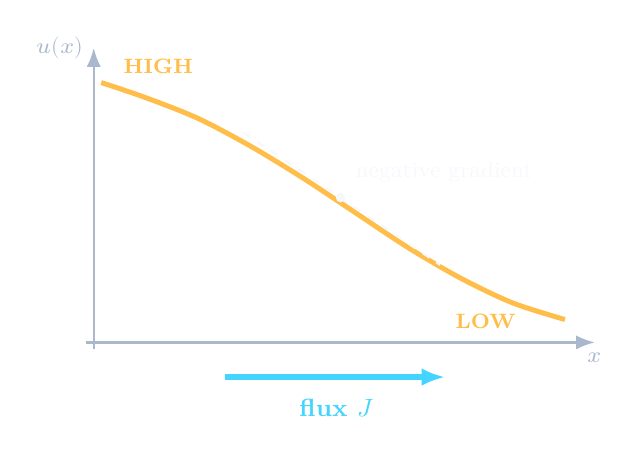
\begin{tikzpicture}[x=0.95cm,y=0.88cm]
        \draw[-{Latex[length=2.4mm]},HydraMuted,line width=0.8pt]
          (0.45,0.55) -- (7.25,0.55)
          node[below,text=HydraMuted,font=\fontsize{8}{9}\selectfont] {$x$};
        \draw[-{Latex[length=2.4mm]},HydraMuted,line width=0.8pt]
          (0.55,0.45) -- (0.55,4.80)
          node[left,text=HydraMuted,font=\fontsize{8}{9}\selectfont] {$u(x)$};

        \draw[HydraGold,line width=1.8pt]
          plot[smooth] coordinates {
            (0.65,4.30) (1.25,4.08) (1.95,3.78) (2.65,3.38)
            (3.35,2.92) (4.05,2.42) (4.75,1.92) (5.45,1.48)
            (6.15,1.12) (6.85,0.88)
          };

        \draw[HydraWhite,dashed,line width=0.8pt]
          (2.55,3.58) -- (5.18,1.67);
        \fill[HydraWhite] (3.85,2.64) circle[radius=0.06cm];
        \node[anchor=south west,text=HydraWhite,
          font=\fontsize{8}{9.5}\selectfont]
          at (3.92,2.72) {negative gradient};

        \node[anchor=south west,text=HydraGold,
          font=\bfseries\fontsize{7.5}{9}\selectfont]
          at (0.82,4.28) {HIGH};
        \node[anchor=south east,text=HydraGold,
          font=\bfseries\fontsize{7.5}{9}\selectfont]
          at (6.32,0.60) {LOW};

        \draw[-{Latex[length=3mm]},HydraCyan,line width=2.2pt]
          (2.30,0.05) -- (5.25,0.05);
        \node[anchor=north,text=HydraCyan,
          font=\bfseries\fontsize{9}{10.5}\selectfont]
          at (3.78,-0.12) {flux $J$};
      \end{tikzpicture}

      \vspace{-0.0cm}

      \begin{columns}[T,totalwidth=\linewidth]
        \begin{column}{0.32\linewidth}
          \centering
          {\color{HydraWhite}\fontsize{8.1}{9.7}\selectfont
            $\partial_xu<0\Rightarrow J>0$
          \par}
          {\color{HydraMuted}\fontsize{6.8}{8.2}\selectfont
            flux to the right
          \par}
        \end{column}

        \begin{column}{0.32\linewidth}
          \centering
          {\color{HydraWhite}\fontsize{8.1}{9.7}\selectfont
            $\partial_xu=0\Rightarrow J=0$
          \par}
          {\color{HydraMuted}\fontsize{6.8}{8.2}\selectfont
            no concentration-driven flux
          \par}
        \end{column}

        \begin{column}{0.32\linewidth}
          \centering
          {\color{HydraWhite}\fontsize{8.1}{9.7}\selectfont
            $|J|=D\,|\partial_xu|$
          \par}
          {\color{HydraMuted}\fontsize{6.8}{8.2}\selectfont
            steeper gradient, larger flux
          \par}
        \end{column}
      \end{columns}

    \end{column}

  \end{columns}

  % \source{
  %   A. Fick, \textit{Ueber Diffusion}, \textit{Annalen der Physik} 170 (1855), 59--86.
  %   Portrait: Anton Klamroth, 1897, Wikimedia Commons (public domain).
  % }

\end{frame}


\begin{frame}{Diffusion equation}

  \vspace{0.02cm}

  \begin{columns}[c,onlytextwidth]
    \begin{column}{0.36\textwidth}
      \centering
      {\color{HydraGold}\bfseries\fontsize{7.6}{9}\selectfont
        LOCAL CONSERVATION\par}
      \vspace{0.04cm}
      {\color{HydraWhite}\fontsize{11.5}{14}\selectfont
        $\partial_tu=-\partial_xJ$
      \par}
    \end{column}

    \begin{column}{0.05\textwidth}
      \centering
      {\color{HydraCyan}\fontsize{15}{15}\selectfont $+$}
    \end{column}

    \begin{column}{0.36\textwidth}
      \centering
      {\color{HydraGold}\bfseries\fontsize{7.6}{9}\selectfont
        FICK'S LAW\par}
      \vspace{0.04cm}
      {\color{HydraWhite}\fontsize{11.5}{14}\selectfont
        $J=-D\partial_xu$
      \par}
    \end{column}
  \end{columns}

  \vspace{0.06cm}

  \begin{center}
    {\color{HydraCyan}\fontsize{16}{16}\selectfont $\Downarrow$\par}

    \vspace{0.66cm}

    {\color{HydraGold}\bfseries\fontsize{8.4}{10}\selectfont
      DIFFUSION EQUATION\par}

    \vspace{0.12cm}

    {\color{HydraWhite}\bfseries\fontsize{20}{24}\selectfont
      $\boxed{\partial_tu=D\partial_{xx}u}$
    \par}
  \end{center}

\end{frame}


\begin{frame}{The diffusion equation on a bounded domain}

  \vspace{0.04cm}

  \begin{columns}[c,onlytextwidth]

    \begin{column}{0.40\textwidth}
      % {\color{HydraGold}\bfseries\fontsize{8}{9.5}\selectfont
        % ONE-DIMENSIONAL PROBLEM\par}

      % \vspace{0.10cm}

      % {\color{HydraMuted}\fontsize{8.2}{10}\selectfont
      %   $x\in(0,L),\qquad t>0$
      % \par}

      % \begin{center}
        {\color{HydraMuted}\fontsize{9}{11}\selectfont
          $\Omega=[0,L]\subset\mathbb{R}$
        \par}
      % \end{center}

      \vspace{-0.52cm}

      {\color{HydraWhite}\fontsize{12.5}{16.5}\selectfont
      \begin{align*}
        \partial_tu(x,t) &= D\,\partial_{xx}u(x,t),
        \\[0.24cm]
        u(x,0) &= u_0(x).
      \end{align*}
      }
    \end{column}

    \begin{column}{0.64\textwidth}
      \centering
      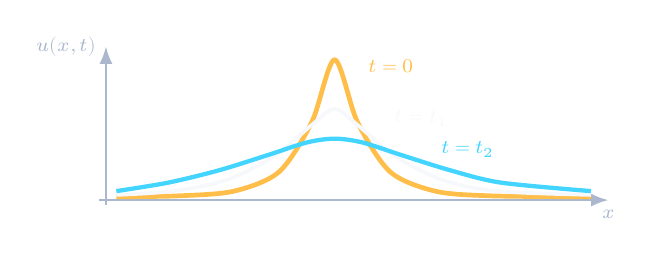
\begin{tikzpicture}[x=0.88cm,y=0.60cm]
        \draw[-{Latex[length=2.2mm]},HydraMuted,line width=0.7pt]
          (0.35,0.45) -- (7.70,0.45)
          node[below,text=HydraMuted,font=\fontsize{7}{8.2}\selectfont] {$x$};
        \draw[-{Latex[length=2.2mm]},HydraMuted,line width=0.7pt]
          (0.45,0.35) -- (0.45,3.70)
          node[left,text=HydraMuted,font=\fontsize{7}{8.2}\selectfont] {$u(x,t)$};

        \draw[HydraGold,line width=1.7pt]
          plot[smooth] coordinates {
            (0.60,0.52) (1.50,0.54) (2.30,0.64) (2.95,1.05)
            (3.42,2.10) (3.75,3.42) (4.08,2.10) (4.55,1.05)
            (5.20,0.64) (6.00,0.54) (7.45,0.52)
          };
        \draw[HydraWhite,line width=1.35pt]
          plot[smooth] coordinates {
            (0.60,0.56) (1.42,0.64) (2.20,0.88) (2.88,1.38)
            (3.42,2.04) (3.75,2.38) (4.08,2.04) (4.62,1.38)
            (5.30,0.88) (6.08,0.64) (7.45,0.56)
          };
        \draw[HydraCyan,line width=1.55pt]
          plot[smooth] coordinates {
            (0.60,0.64) (1.35,0.82) (2.08,1.08) (2.78,1.40)
            (3.35,1.67) (3.75,1.75) (4.15,1.67) (4.72,1.40)
            (5.42,1.08) (6.15,0.82) (7.45,0.64)
          };

        \node[anchor=west,text=HydraGold,
          font=\bfseries\fontsize{7}{8.2}\selectfont]
          at (4.10,3.28) {$t=0$};
        \node[anchor=west,text=HydraWhite,
          font=\bfseries\fontsize{7}{8.2}\selectfont]
          at (4.48,2.18) {$t=t_1$};
        \node[anchor=west,text=HydraCyan,
          font=\bfseries\fontsize{7}{8.2}\selectfont]
          at (5.15,1.52) {$t=t_2$};
      \end{tikzpicture}
    \end{column}

  \end{columns}

  \vspace{0.98cm}

  \begin{columns}[T,onlytextwidth]

    \begin{column}{0.47\textwidth}
      \HydraPoint[HydraCyan]
        {No-flux boundary (Neumann)}
        {The sealed ends prevent the substance from leaving}

      \vspace{0.05cm}

      \centering
      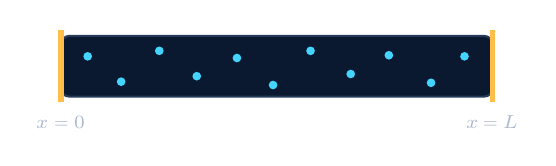
\begin{tikzpicture}[x=0.85cm,y=0.70cm]
        \fill[HydraPanel,rounded corners=3pt]
          (0.55,0.55) rectangle (7.00,1.65);
        \draw[HydraLine,line width=0.75pt,rounded corners=3pt]
          (0.55,0.55) rectangle (7.00,1.65);

        \draw[HydraGold,line width=2.0pt]
          (0.55,0.45) -- (0.55,1.75);
        \draw[HydraGold,line width=2.0pt]
          (7.00,0.45) -- (7.00,1.75);

        \foreach \px/\py in {0.95/1.28,1.45/0.82,2.02/1.38,2.58/0.92,
          3.18/1.25,3.72/0.76,4.28/1.38,4.88/0.96,5.45/1.30,6.08/0.80,6.58/1.28}{
          \fill[HydraCyan] (\px,\py) circle[radius=0.055cm];
        }

        \node[anchor=north,text=HydraMuted,
          font=\fontsize{6.8}{8}\selectfont] at (0.55,0.38) {$x=0$};
        \node[anchor=north,text=HydraMuted,
          font=\fontsize{6.8}{8}\selectfont] at (7.00,0.38) {$x=L$};
      \end{tikzpicture}
      \vspace{-0.4cm}
      {\color{HydraWhite}\fontsize{9.2}{11.5}\selectfont
      \begin{align*}
        \partial_xu(0,t) &= 0
        &
        \partial_xu(L,t) &= 0
      \end{align*}
      }
    \end{column}

    \begin{column}{0.47\textwidth}
      \HydraPoint[HydraGold]
        {Absorbing boundary (Dirichlet)}
        {Substance that reaches an open end leaves the domain}

      \vspace{0.05cm}

      \centering
      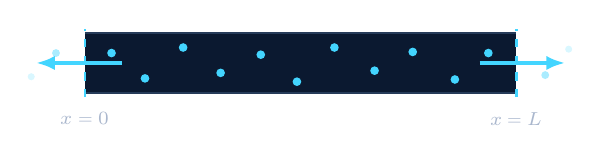
\begin{tikzpicture}[x=0.85cm,y=0.70cm]
        \fill[HydraPanel]
          (0.55,0.55) rectangle (7.00,1.65);
        \draw[HydraLine,line width=0.75pt]
          (0.55,0.55) -- (7.00,0.55);
        \draw[HydraLine,line width=0.75pt]
          (0.55,1.65) -- (7.00,1.65);

        \draw[HydraCyan,dashed,line width=0.8pt]
          (0.55,0.48) -- (0.55,1.72);
        \draw[HydraCyan,dashed,line width=0.8pt]
          (7.00,0.48) -- (7.00,1.72);

        \draw[-{Latex[length=2.4mm]},HydraCyan,line width=1.4pt]
          (1.10,1.10) -- (-0.18,1.10);
        \draw[-{Latex[length=2.4mm]},HydraCyan,line width=1.4pt]
          (6.45,1.10) -- (7.73,1.10);

        \foreach \px/\py in {0.95/1.28,1.45/0.82,2.02/1.38,2.58/0.92,
          3.18/1.25,3.72/0.76,4.28/1.38,4.88/0.96,5.45/1.30,6.08/0.80,6.58/1.28}{
          \fill[HydraCyan] (\px,\py) circle[radius=0.055cm];
        }

        \fill[HydraCyan,opacity=0.45] (0.12,1.28) circle[radius=0.05cm];
        \fill[HydraCyan,opacity=0.20] (-0.25,0.85) circle[radius=0.045cm];
        \fill[HydraCyan,opacity=0.45] (7.43,0.88) circle[radius=0.05cm];
        \fill[HydraCyan,opacity=0.20] (7.78,1.35) circle[radius=0.045cm];

        \node[anchor=north,text=HydraMuted,
          font=\fontsize{6.8}{8}\selectfont] at (0.55,0.38) {$x=0$};
        \node[anchor=north,text=HydraMuted,
          font=\fontsize{6.8}{8}\selectfont] at (7.00,0.38) {$x=L$};
      \end{tikzpicture}
      \vspace{-0.8cm}
      {\color{HydraWhite}\fontsize{9.2}{11.5}\selectfont
      \begin{align*}
        u(0,t) &= 0,
        &
        u(L,t) &= 0.
      \end{align*}
      }
    \end{column}

  \end{columns}

\end{frame}


\begin{frame}{Fourier turns diffusion into a problem of spatial modes}

  \vspace{-0.04cm}

  \begin{columns}[c,onlytextwidth]

    \begin{column}{0.38\textwidth}
      {\color{HydraGold}\bfseries\fontsize{17}{19}\selectfont
        1822\par}

      \vspace{0.04cm}

      {\color{HydraWhite}\bfseries\fontsize{10.2}{12.5}\selectfont
        \textit{Théorie analytique de la chaleur}\par}

      \vspace{0.10cm}

      \HydraPoint[HydraGold]
        {Fourier's question}
        {How does an arbitrary temperature profile evolve under the heat equation?}

      \vspace{0.08cm}

      \HydraPoint[HydraCyan]
        {The key idea}
        {Decompose a complicated spatial profile into simple sine and cosine waves.}

      \vspace{0.08cm}

      {\color{HydraWhite}\fontsize{9.4}{12.2}\selectfont
      \[
        u_0(x)
        =a_0+\sum_{n=1}^{\infty}
        a_n\cos\!\left(\frac{n\pi x}{L}\right).
      \]
      }
    \end{column}

    \begin{column}{0.57\textwidth}
      \centering
      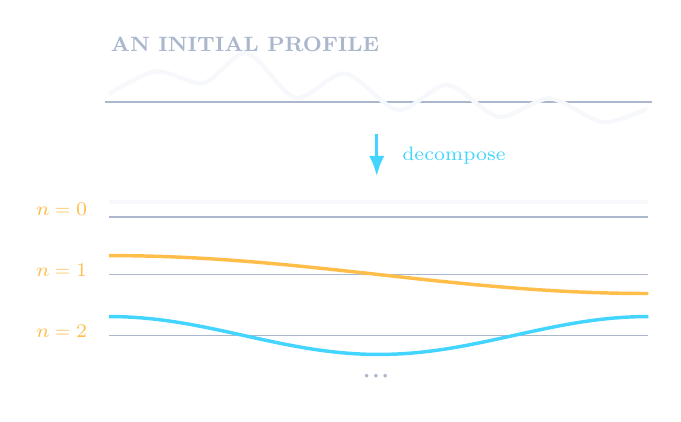
\begin{tikzpicture}[x=1cm,y=0.86cm]
        \node[anchor=west,text=HydraMuted,
          font=\bfseries\fontsize{7.5}{9}\selectfont]
          at (0.25,5.15) {AN INITIAL PROFILE};

        \draw[HydraMuted,line width=0.55pt]
          (0.30,4.30) -- (7.25,4.30);
        \draw[HydraWhite,line width=1.55pt]
          plot[smooth] coordinates {
            (0.35,4.42) (0.95,4.75) (1.55,4.58) (2.10,5.02)
            (2.72,4.36) (3.35,4.72) (4.02,4.18) (4.65,4.55)
            (5.30,4.08) (5.95,4.35) (6.62,4.00) (7.18,4.20)
          };

        \draw[-{Latex[length=2.6mm]},HydraCyan,line width=1.2pt]
          (3.75,3.82) -- (3.75,3.20);
        \node[anchor=west,text=HydraCyan,
          font=\fontsize{7}{8.5}\selectfont]
          at (3.95,3.50) {decompose};

        \node[anchor=east,text=HydraGold,
          font=\bfseries\fontsize{7}{8.5}\selectfont]
          at (0.20,2.72) {$n=0$};
        \draw[HydraMuted,line width=0.45pt]
          (0.35,2.60) -- (7.20,2.60);
        \draw[HydraWhite,line width=1.25pt]
          (0.35,2.82) -- (7.20,2.82);

        \node[anchor=east,text=HydraGold,
          font=\bfseries\fontsize{7}{8.5}\selectfont]
          at (0.20,1.82) {$n=1$};
        \draw[HydraMuted,line width=0.45pt]
          (0.35,1.75) -- (7.20,1.75);
        \draw[HydraGold,line width=1.25pt]
          plot[domain=0.35:7.20,samples=80]
          (\x,{1.75+0.28*cos(180*(\x-0.35)/6.85)});

        \node[anchor=east,text=HydraGold,
          font=\bfseries\fontsize{7}{8.5}\selectfont]
          at (0.20,0.92) {$n=2$};
        \draw[HydraMuted,line width=0.45pt]
          (0.35,0.85) -- (7.20,0.85);
        \draw[HydraCyan,line width=1.25pt]
          plot[domain=0.35:7.20,samples=80]
          (\x,{0.85+0.28*cos(360*(\x-0.35)/6.85)});

        \node[text=HydraMuted,font=\fontsize{12}{12}\selectfont]
          at (3.75,0.20) {$\cdots$};
      \end{tikzpicture}

      \vspace{0.02cm}

      {\color{HydraMuted}\fontsize{7.4}{9}\selectfont
        Instead of solving for every initial profile separately,
        solve how each elementary spatial wave evolves.
      \par}
    \end{column}

  \end{columns}



\end{frame}


\begin{frame}{No-flux boundaries --- cosine modes}

  \vspace{-0.04cm}

  \begin{columns}[c,onlytextwidth]

    \begin{column}{0.43\textwidth}
      \HydraPoint[HydraCyan]
        {A mode keeps its spatial shape}
        {Applying the diffusion operator changes only its amplitude, not the form of the profile.}

      \vspace{0.06cm}

      {\color{HydraWhite}\fontsize{10.2}{13}\selectfont
      \begin{align*}
        -\phi_n'' &= \mu_n\phi_n,
        \\[0.10cm]
        \phi_n'(0) &= \phi_n'(L)=0.
      \end{align*}
      }

      \vspace{-0.04cm}

      {\color{HydraWhite}\fontsize{10}{12.8}\selectfont
      \begin{align*}
        \phi_n(x)
        &=\cos\!\left(\frac{n\pi x}{L}\right),
        \\[0.10cm]
        \mu_n
        &=\left(\frac{n\pi}{L}\right)^2.
      \end{align*}
      }

      \vspace{0.02cm}

      {\color{HydraMuted}\fontsize{7.5}{9.1}\selectfont
        The derivative vanishes at both endpoints, so every cosine
        satisfies the no-flux boundary conditions.
      \par}
    \end{column}

    \begin{column}{0.53\textwidth}
      \centering
      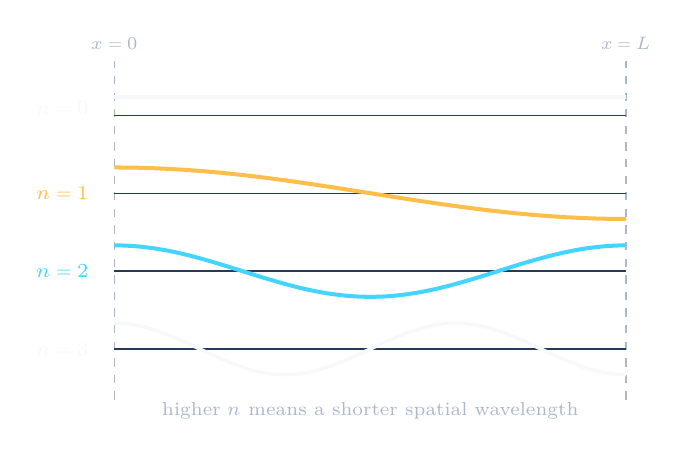
\begin{tikzpicture}[x=1cm,y=0.86cm]
        \draw[HydraMuted,dashed,line width=0.55pt]
          (0.55,0.25) -- (0.55,5.25);
        \draw[HydraMuted,dashed,line width=0.55pt]
          (7.05,0.25) -- (7.05,5.25);

        \node[anchor=south,text=HydraMuted,
          font=\fontsize{6.5}{7.8}\selectfont] at (0.55,5.28) {$x=0$};
        \node[anchor=south,text=HydraMuted,
          font=\fontsize{6.5}{7.8}\selectfont] at (7.05,5.28) {$x=L$};

        \draw[HydraLine,line width=0.45pt] (0.55,4.45) -- (7.05,4.45);
        \draw[HydraWhite,line width=1.35pt] (0.55,4.72) -- (7.05,4.72);
        \node[anchor=east,text=HydraWhite,
          font=\bfseries\fontsize{7.2}{8.7}\selectfont] at (0.35,4.55) {$n=0$};

        \draw[HydraLine,line width=0.45pt] (0.55,3.30) -- (7.05,3.30);
        \draw[HydraGold,line width=1.45pt]
          plot[domain=0.55:7.05,samples=100]
          (\x,{3.30+0.38*cos(180*(\x-0.55)/6.50)});
        \node[anchor=east,text=HydraGold,
          font=\bfseries\fontsize{7.2}{8.7}\selectfont] at (0.35,3.30) {$n=1$};

        \draw[HydraLine,line width=0.45pt] (0.55,2.15) -- (7.05,2.15);
        \draw[HydraCyan,line width=1.45pt]
          plot[domain=0.55:7.05,samples=100]
          (\x,{2.15+0.38*cos(360*(\x-0.55)/6.50)});
        \node[anchor=east,text=HydraCyan,
          font=\bfseries\fontsize{7.2}{8.7}\selectfont] at (0.35,2.15) {$n=2$};

        \draw[HydraLine,line width=0.45pt] (0.55,1.00) -- (7.05,1.00);
        \draw[HydraWhite,line width=1.30pt]
          plot[domain=0.55:7.05,samples=100]
          (\x,{1.00+0.38*cos(540*(\x-0.55)/6.50)});
        \node[anchor=east,text=HydraWhite,
          font=\bfseries\fontsize{7.2}{8.7}\selectfont] at (0.35,1.00) {$n=3$};

        \node[anchor=north,text=HydraMuted,
          font=\fontsize{6.8}{8.2}\selectfont]
          at (3.80,0.35) {higher $n$ means a shorter spatial wavelength};
      \end{tikzpicture}
    \end{column}

  \end{columns}

\end{frame}


\begin{frame}{Eigenfunctions and eigenmodes}

  \vspace{-0.24cm}

  \begin{columns}[c,onlytextwidth]

    \begin{column}{0.56\textwidth}

      \begin{columns}[c,totalwidth=\linewidth]
        \begin{column}{0.57\linewidth}
          {\color{HydraWhite}\fontsize{9.2}{11.8}\selectfont
          \[
            u(x,t)=\sum_{n=0}^{\infty}a_n(t)\phi_n(x)
          \]
          }
        \end{column}

        \begin{column}{0.40\linewidth}
          {\color{HydraMuted}\fontsize{6.9}{8.5}\selectfont
          \begin{align*}
            \phi_n(x)
            &=\cos\!\left(\frac{n\pi x}{L}\right)
            \\
            \mu_n
            &=\left(\frac{n\pi}{L}\right)^2
          \end{align*}
          }
        \end{column}
      \end{columns}

      \vspace{-0.38cm}


      {\color{HydraWhite}\fontsize{8.9}{11.5}\selectfont
      \begin{align*}
        -\phi_n'' &= \mu_n\phi_n
        &
        \phi_n'(0)&=\phi_n'(L)=0
      \end{align*}
      }

      \vspace{-0.68cm}


      {\color{HydraWhite}\fontsize{8.8}{11.3}\selectfont
      \begin{align*}
        \partial_t u(x,t) = \sum_{n=0}^{\infty}a_n'(t)\phi_n
        &=D\sum_{n=0}^{\infty}a_n(t)\phi_n'' = D\,\partial_{xx} u(x,t)
      \end{align*}
      }

      \vspace{-0.22cm}

      {\color{HydraWhite}\fontsize{9.6}{12.2}\selectfont
      \[
        \boxed{
          \begin{aligned}
            a_n'(t)&=-D\mu_n a_n(t)
            \\
            a_n(t)&=a_n(0)e^{-D\mu_nt}
          \end{aligned}
        }
      \]
      }

      \vspace{-0.18cm}

    \end{column}

    \begin{column}{0.40\textwidth}
      \centering
      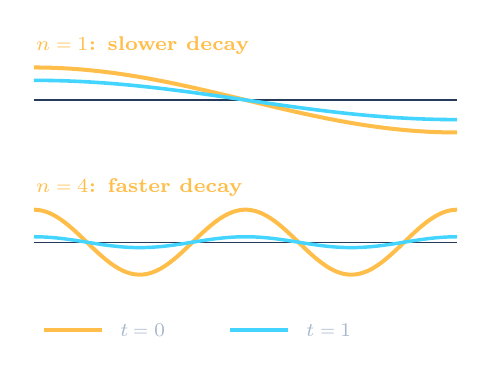
\begin{tikzpicture}[x=0.86cm,y=0.86cm]
        \node[anchor=west,text=HydraGold,
          font=\bfseries\fontsize{7.2}{8.7}\selectfont]
          at (0.15,4.75) {$n=1$: slower decay};
        \draw[HydraLine,line width=0.45pt] (0.25,3.95) -- (6.50,3.95);
        \draw[HydraGold,line width=1.45pt]
          plot[domain=0.25:6.50,samples=90]
          (\x,{3.95+0.48*cos(180*(\x-0.25)/6.25)});
        \draw[HydraCyan,line width=1.30pt]
          plot[domain=0.25:6.50,samples=90]
          (\x,{3.95+0.29*cos(180*(\x-0.25)/6.25)});

        \node[anchor=west,text=HydraGold,
          font=\bfseries\fontsize{7.2}{8.7}\selectfont]
          at (0.15,2.65) {$n=4$: faster decay};
        \draw[HydraLine,line width=0.45pt] (0.25,1.85) -- (6.50,1.85);
        \draw[HydraGold,line width=1.45pt]
          plot[domain=0.25:6.50,samples=110]
          (\x,{1.85+0.48*cos(720*(\x-0.25)/6.25)});
        \draw[HydraCyan,line width=1.25pt]
          plot[domain=0.25:6.50,samples=110]
          (\x,{1.85+0.08*cos(720*(\x-0.25)/6.25)});

        \draw[HydraGold,line width=1.35pt] (0.40,0.55) -- (1.25,0.55);
        \node[anchor=west,text=HydraMuted,
          font=\fontsize{7}{8.3}\selectfont] at (1.38,0.55) {$t=0$};
        \draw[HydraCyan,line width=1.35pt] (3.15,0.55) -- (4.00,0.55);
        \node[anchor=west,text=HydraMuted,
          font=\fontsize{7}{8.3}\selectfont] at (4.13,0.55) {$t=1$};
      \end{tikzpicture}

      \vspace{0.00cm}

      \HydraPoint[HydraCyan]
        {Short waves disappear first}
        {Because $\mu_n=(n\pi/L)^2$, modes with larger $n$ decay much faster.}



    \end{column}

  \end{columns}

\end{frame}




\begin{frame}{Diffusion in higher dimensions}

  \vspace{0.15cm}

  \begin{columns}[c,onlytextwidth]

    \begin{column}{0.56\textwidth}
      {\color{HydraWhite}\fontsize{13.5}{18}\selectfont
      \[
        x\in\Omega\subset\mathbb{R}^{d}
        \qquad
        \partial_tu=D\Delta u
      \]
      }

      \vspace{0.18cm}

      {\color{HydraMuted}\fontsize{9.2}{12}\selectfont
        In Cartesian coordinates,
      \par}

      {\color{HydraWhite}\fontsize{12.5}{17}\selectfont
      \[
        \Delta u
        =
        \partial_{x_1x_1}u+\cdots+\partial_{x_dx_d}u
      \]
      }

      \vspace{0.20cm}

      \HydraPoint[HydraCyan]
        {No-flux boundary}
        {A closed tissue does not allow the signal to cross its boundary.}

      \vspace{-0.05cm}

      {\color{HydraWhite}\fontsize{12.5}{16}\selectfont
      \[
        \nabla u\cdot n=0
        \qquad\text{on }\partial\Omega
      \]
      }
    \end{column}

    \begin{column}{0.40\textwidth}
      \centering
      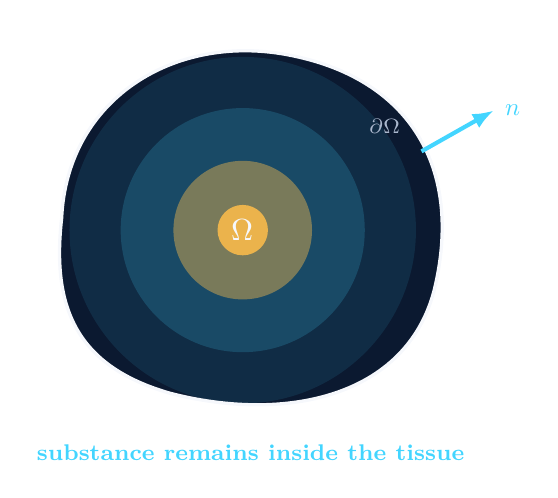
\begin{tikzpicture}[x=1cm,y=1cm]
        \begin{scope}
          \clip
            (0.35,2.70)
            .. controls (0.42,4.25) and (1.85,5.10) .. (3.35,4.75)
            .. controls (4.82,4.42) and (5.45,3.28) .. (5.08,1.78)
            .. controls (4.72,0.42) and (3.18,0.10) .. (1.72,0.48)
            .. controls (0.55,0.82) and (0.22,1.55) .. cycle;

          \fill[HydraPanel] (-0.1,-0.1) rectangle (5.7,5.3);
          \fill[HydraCyan,opacity=0.10] (2.65,2.55) circle[radius=2.20cm];
          \fill[HydraCyan,opacity=0.18] (2.65,2.55) circle[radius=1.55cm];
          \fill[HydraGold,opacity=0.42] (2.65,2.55) circle[radius=0.88cm];
          \fill[HydraGold,opacity=0.85] (2.65,2.55) circle[radius=0.32cm];
        \end{scope}

        \draw[HydraWhite,line width=1.2pt]
          (0.35,2.70)
          .. controls (0.42,4.25) and (1.85,5.10) .. (3.35,4.75)
          .. controls (4.82,4.42) and (5.45,3.28) .. (5.08,1.78)
          .. controls (4.72,0.42) and (3.18,0.10) .. (1.72,0.48)
          .. controls (0.55,0.82) and (0.22,1.55) .. cycle;

        \node[text=HydraWhite,font=\bfseries\fontsize{11}{13}\selectfont]
          at (2.65,2.55) {$\Omega$};

        \coordinate (boundarypoint) at (4.92,3.55);
        \draw[-{Latex[length=2.7mm]},HydraCyan,line width=1.5pt]
          (boundarypoint) -- ++(0.92,0.52)
          node[anchor=west,text=HydraCyan,
            font=\bfseries\fontsize{9}{10.5}\selectfont] {$n$};
        \node[anchor=south east,text=HydraMuted,
          font=\fontsize{7.5}{9}\selectfont]
          at (4.78,3.65) {$\partial\Omega$};

        \node[anchor=north,text=HydraCyan,
          font=\bfseries\fontsize{8.2}{9.8}\selectfont]
          at (2.75,-0.05) {substance remains inside the tissue};
      \end{tikzpicture}
    \end{column}

  \end{columns}

\end{frame}


\begin{frame}{Eigenfunctions on a bounded domain}

  \vspace{-0.04cm}

  \begin{center}
    \begin{minipage}{0.91\textwidth}
      {\color{HydraGold}\bfseries\fontsize{7.2}{8.6}\selectfont
        THEOREM\par}

      \vspace{0.04cm}

      {\color{HydraWhite}\fontsize{8}{9.7}\selectfont
        There exist eigenfunctions $\{\phi_k\}_{k=0}^{\infty}$ and eigenvalues $\{\mu_k\}_{k=0}^{\infty}$ of the Laplace operator  satisfying
      \par}

      {\color{HydraWhite}\fontsize{10.2}{13}\selectfont
      \[
        -\Delta\phi_k=\mu_k\phi_k,
        \qquad
        \nabla\phi_k\cdot n=0
        \quad\text{on }\partial\Omega.
      \]
      }

      \vspace{-0.52cm}

      {\color{HydraWhite}\fontsize{9.8}{12.4}\selectfont
      \[
        0=\mu_0<\mu_1\leq\mu_2\leq\cdots,
        \qquad
        \boxed{\mu_k\longrightarrow\infty}.
      \]
      }

      \vspace{-0.10cm}

      {\color{HydraMuted}\fontsize{7.5}{9.1}\selectfont
        The eigenfunctions form an orthonormal basis, solution can be written as a sum of spatial modes.
      \par}
    \end{minipage}
  \end{center}

  \vspace{0.00cm}

  \begin{columns}[c,onlytextwidth]
    \begin{column}{0.57\textwidth}
      {\color{HydraWhite}\fontsize{9.4}{12.2}\selectfont
      \begin{align*}
        u_0(x)
        &=\sum_{k=0}^{\infty}a_k(0)\phi_k(x),
        \\[0.12cm]
        u(x,t)
        &=\sum_{k=0}^{\infty}
          a_k(0)e^{-D\mu_kt}\phi_k(x).
      \end{align*}
      }
    \end{column}

    \begin{column}{0.38\textwidth}
      \HydraPoint[HydraCyan]
        {Different modes, different rates}
        {Large eigenvalues correspond to rapidly decaying spatial structure.}

      \vspace{0.08cm}

      \HydraPoint[HydraGold]
        {No mode is amplified}
        {Every nonconstant mode decreases under diffusion alone.}
    \end{column}
  \end{columns}

  \vspace{0.02cm}

  \HydraTakeaway{
    Diffusion alone damps spatial variation
  }

\end{frame}

\HydraSubsection[
  \mbox{Reactions change signals locally}
  \mbox{through production, degradation}
  \mbox{and nonlinear interactions}
]{Local dynamics}

\begin{frame}{Reaction}

  \vspace{-0.16cm}

  \begin{columns}[c,onlytextwidth]

    \begin{column}{0.58\textwidth}
      {\color{HydraMuted}\fontsize{8.2}{10.2}\selectfont
        Begin with a system of ordinary differential equations
      \par}

      \vspace{-0.22cm}

      {\color{HydraWhite}\fontsize{10.4}{13.2}\selectfont
      \begin{align*}
        \partial_t u&=f(u,v)
        \\
        \partial_t v&=g(u,v)
      \end{align*}
      }

      \vspace{-0.28cm}

      {\color{HydraWhite}\fontsize{8.2}{10.2}\selectfont
        $u$ and $v$ are the local concentrations of two substances
      \par}

      \vspace{0.10cm}

      {\color{HydraMuted}\fontsize{8.2}{10.2}\selectfont
        The functions $f(u,v)$ and $g(u,v)$ describe how these
        concentrations change depending on their current values
      \par}

      \vspace{0.24cm}

      \HydraPoint[HydraGold]
        {One state at every position}
        {The pair $(u,v)$ represents the local chemical state.}

      \vspace{-0.28cm}

    \end{column}

    \begin{column}{0.38\textwidth}
      \centering

      % REPLACEABLE VISUAL
      % Replace the tikzpicture with:
      % \includegraphics[width=\linewidth,height=5.25cm,keepaspectratio]{figures/local_dynamics/...}
      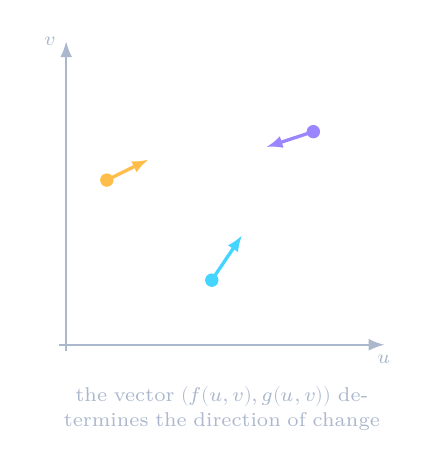
\begin{tikzpicture}[x=0.86cm,y=0.82cm]

        \draw[-{Latex[length=2mm]},HydraMuted,line width=0.75pt]
          (0.45,0.55) -- (5.25,0.55)
          node[below,text=HydraMuted,
            font=\fontsize{7}{8.2}\selectfont] {$u$};

        \draw[-{Latex[length=2mm]},HydraMuted,line width=0.75pt]
          (0.55,0.45) -- (0.55,5.25)
          node[left,text=HydraMuted,
            font=\fontsize{7}{8.2}\selectfont] {$v$};

        \fill[HydraGold]
          (1.15,3.10) circle[radius=0.085cm];

        \fill[HydraCyan]
          (2.70,1.55) circle[radius=0.085cm];

        \fill[HydraViolet]
          (4.20,3.85) circle[radius=0.085cm];

        \draw[-{Latex[length=2.1mm]},HydraGold,line width=1.2pt]
          (1.15,3.10) -- ++(0.62,0.32);

        \draw[-{Latex[length=2.1mm]},HydraCyan,line width=1.2pt]
          (2.70,1.55) -- ++(0.45,0.70);

        \draw[-{Latex[length=2.1mm]},HydraViolet,line width=1.2pt]
          (4.20,3.85) -- ++(-0.70,-0.24);

        \node[anchor=north,text=HydraMuted,
          text width=4.7cm,align=center,
          font=\fontsize{7.2}{8.8}\selectfont]
          at (2.85,0.05)
          {the vector $(f(u,v),g(u,v))$ determines the direction of change};

      \end{tikzpicture}
    \end{column}

  \end{columns}

\end{frame}


\begin{frame}{Reaction --- vector field and trajectory}

  \vspace{-0.04cm}

  \begin{columns}[c,onlytextwidth]

    \begin{column}{0.43\textwidth}
      {\color{HydraWhite}\fontsize{11.6}{14.6}\selectfont
      \[
        \begin{aligned}
          \partial_t u&=f(u,v)
          \\
          \partial_t v&=g(u,v)
        \end{aligned}
      \]
      }

      \vspace{-0.14cm}

      {\color{HydraMuted}\fontsize{8.2}{10.2}\selectfont
        supplemented with initial conditions
      \par}

      \vspace{-0.22cm}

      {\color{HydraWhite}\fontsize{10.2}{13}\selectfont
      \[
        u_0=u(0)
        \qquad
        v_0=v(0)
      \]
      }

      \vspace{-0.24cm}

      \HydraPoint[HydraGold]
        {Initial state}
        {The pair $(u_0,v_0)$ selects the starting point in the concentration plane.}

      \vspace{-0.10cm}

      \HydraPoint[HydraCyan]
        {Velocity}
        {The vector $(f(u,v),g(u,v))$ gives the instantaneous direction of change.}

      \vspace{-0.10cm}

      \HydraPoint[HydraGold]
        {Trajectory}
        {The solution curve is tangent to the vector field at every point.}
    \end{column}

    \begin{column}{0.53\textwidth}
      
      % \vspace{3.58cm}
      \centering

      % REPLACEABLE VISUAL
      % Replace the placeholder with:
      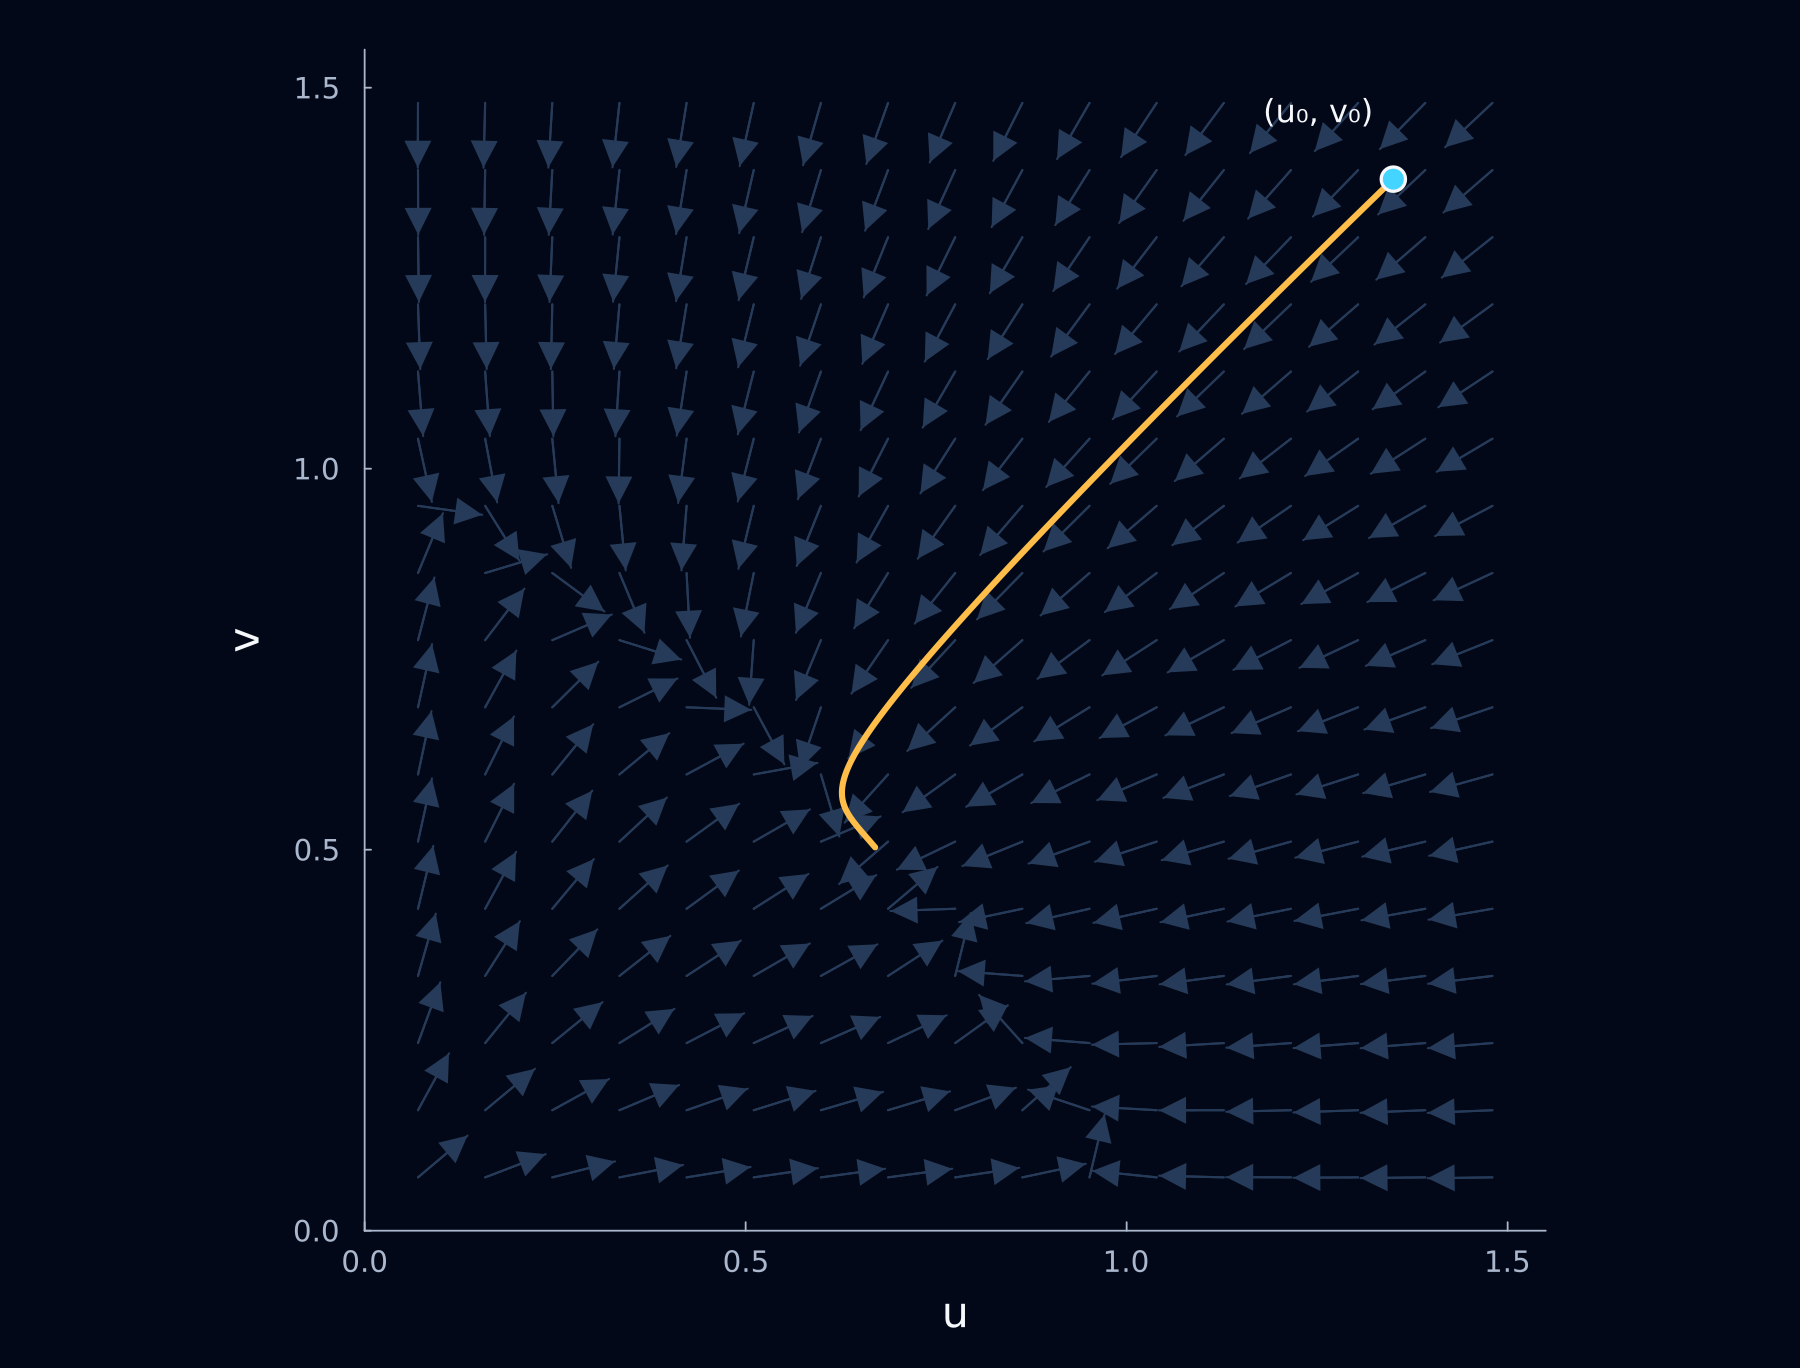
\includegraphics[
        width=\linewidth,
        height=5.45cm,
        keepaspectratio
      ]{figures/local_dynamics/vector_field.png}

      % \begin{tikzpicture}
      %   \node[
      %     draw=HydraLine,
      %     rounded corners=2pt,
      %     minimum width=0.94\linewidth,
      %     minimum height=5.25cm,
      %     align=center,
      %     text=HydraMuted,
      %     font=\fontsize{8}{10}\selectfont
      %   ] {
      %     vector field and trajectory
      %     \\
      %     \vspace{0.08cm}
      %     {\fontsize{6.8}{8.2}\selectfont
      %       replace with your own plot}
      %   };
      % \end{tikzpicture}
    \end{column}

  \end{columns}

\end{frame}

\begin{frame}{Steady state}

  \vspace{-0.12cm}

  \begin{columns}[c,onlytextwidth]


    
    \begin{column}{0.46\textwidth}
            {\color{HydraMuted}\fontsize{8.1}{10.2}\selectfont
        At a steady state $u(t)\equiv\bar u$, $v(t)\equiv\bar v$, both concentrations remain constant in time
      \par}


      {\color{HydraWhite}\fontsize{11.2}{14.2}\selectfont
      \[
        \begin{aligned}
          f(\bar u,\bar v)&=0
          &\qquad
          g(\bar u,\bar v)&=0
        \end{aligned}
      \]
      }

      \vspace{-0.22cm}


      \vspace{0.34cm}

      {\color{HydraWhite}\bfseries\fontsize{8}{9.6}\selectfont
        NULLCLINES\par}

      \vspace{-0.10cm}

      {\color{HydraWhite}\fontsize{11}{14}\selectfont
      \begin{align*}
        \textcolor{HydraCyan}{f(u,v)=0}
        &&
        \text{\color{HydraMuted}\fontsize{7.6}{9}\selectfont
          $u$ does not change}
        \\
        \textcolor{HydraGold}{g(u,v)=0}
        &&
        \text{\color{HydraMuted}\fontsize{7.6}{9}\selectfont
          $v$ does not change}
      \end{align*}
      }

      \vspace{-0.12cm}

      {\color{HydraMuted}\fontsize{8.1}{10.2}\selectfont
        Each nullcline contains states for which one concentration
        is instantaneously stationary
      \par}


    \end{column}

    \begin{column}{0.50\textwidth}
      \centering

      % REPLACEABLE VISUAL
      % Replace the tikzpicture with:
      % \includegraphics[
      %   width=\linewidth,
      %   height=5.40cm,
      %   keepaspectratio
      % ]{figures/local_dynamics/nullclines.png}

      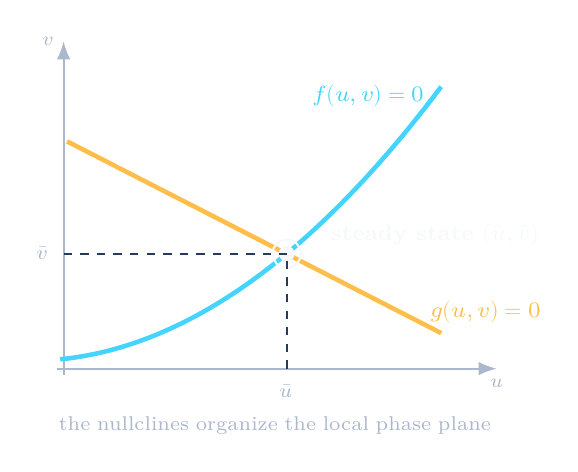
\begin{tikzpicture}[x=0.88cm,y=0.82cm]
        \draw[-{Latex[length=2.3mm]},HydraMuted,line width=0.75pt]
          (0.40,0.48) -- (6.75,0.48)
          node[below,text=HydraMuted,
            font=\fontsize{7}{8.2}\selectfont] {$u$};

        \draw[-{Latex[length=2.3mm]},HydraMuted,line width=0.75pt]
          (0.50,0.38) -- (0.50,5.55)
          node[left,text=HydraMuted,
            font=\fontsize{7}{8.2}\selectfont] {$v$};

        \draw[
          HydraCyan,
          line width=1.65pt,
          domain=0.45:5.95,
          samples=90
        ]
          plot (\x,{0.60+0.12*\x*\x});

        \draw[HydraGold,line width=1.65pt]
          (0.55,4.00) -- (5.95,1.03);

        \node[
          anchor=west,
          text=HydraCyan,
          font=\bfseries\fontsize{8}{9.5}\selectfont
        ]
          at (3.95,4.70) {$f(u,v)=0$};

        \node[
          anchor=west,
          text=HydraGold,
          font=\bfseries\fontsize{8}{9.5}\selectfont
        ]
          at (5.65,1.35) {$g(u,v)=0$};

        \fill[HydraWhite]
          (3.72,2.26) circle[radius=0.10cm];

        \draw[HydraWhite,line width=0.75pt]
          (3.72,2.26) circle[radius=0.18cm];

        \node[
          anchor=south west,
          text=HydraWhite,
          font=\bfseries\fontsize{8}{9.5}\selectfont
        ]
          at (4.22,2.23)
          {steady state $(\bar u,\bar v)$};

        \draw[dashed,HydraLine,line width=0.65pt]
          (3.72,0.48) -- (3.72,2.26);

        \draw[dashed,HydraLine,line width=0.65pt]
          (0.50,2.26) -- (3.72,2.26);

        \node[
          anchor=north,
          text=HydraMuted,
          font=\fontsize{7.2}{8.8}\selectfont
        ]
          at (3.72,0.38) {$\bar u$};

        \node[
          anchor=east,
          text=HydraMuted,
          font=\fontsize{7.2}{8.8}\selectfont
        ]
          at (0.42,2.26) {$\bar v$};

        \node[
          anchor=north,
          text=HydraMuted,
          text width=5.6cm,
          align=center,
          font=\fontsize{7.2}{8.8}\selectfont
        ]
          at (3.55,-0.12)
          {the nullclines organize the local phase plane};
      \end{tikzpicture}
    \end{column}

  \end{columns}

\end{frame}


\begin{frame}{Lyapunov stability}

  \vspace{-0.54cm}

  \begin{columns}[c,onlytextwidth]

    \begin{column}{0.44\textwidth}
      {\color{HydraMuted}\fontsize{7.8}{9.6}\selectfont
        Consider two solutions of the same system
      \par}

      \vspace{-0.18cm}

      {\color{HydraWhite}\fontsize{9.7}{12.4}\selectfont
      \begin{align*}
        \partial_t u&=f(u,v)
        \\
        \partial_t v&=g(u,v)
      \end{align*}
      }

      \vspace{-1.28cm}

      {\fontsize{8.8}{11.2}\selectfont
      \begin{align*}
        \textcolor{HydraCyan}{u(0)}
        &\textcolor{HydraCyan}{=u_0}
        &
        \textcolor{HydraGold}{\widetilde u(0)}
        &\textcolor{HydraGold}{=\widetilde u_0}
        \\
        \textcolor{HydraCyan}{v(0)}
        &\textcolor{HydraCyan}{=v_0}
        &
        \textcolor{HydraGold}{\widetilde v(0)}
        &\textcolor{HydraGold}{=\widetilde v_0}
      \end{align*}
      }
      \par
      \vspace{0.1cm}

      {\color{HydraGold}\bfseries\fontsize{7.7}{9.2}\selectfont
        LYAPUNOV STABILITY\par}

      % \vspace{-0.10cm}

      {\color{HydraWhite}\fontsize{7.5}{9.3}\selectfont
        For every $\varepsilon>0$ there exists $\delta>0$ such that
      \par}

      \vspace{-0.42cm}

{\color{HydraWhite}\fontsize{9.4}{12}\selectfont
\begin{align*}
  \left\|
    (u_0,v_0)-(\widetilde u_0,\widetilde v_0)
  \right\|&<\delta
  \quad \Rightarrow  \\ 
  \left\|
    (u(t),v(t))-(\widetilde u(t),\widetilde v(t))
  \right\|&<\varepsilon
  \qquad
  \text{for all } t\geq0
\end{align*}
}
      \par
      \vspace{-0.26cm}

    \end{column}

    \begin{column}{0.52\textwidth}

        \begin{columns}[c,onlytextwidth]

          \begin{column}{0.72\linewidth}
            \centering

            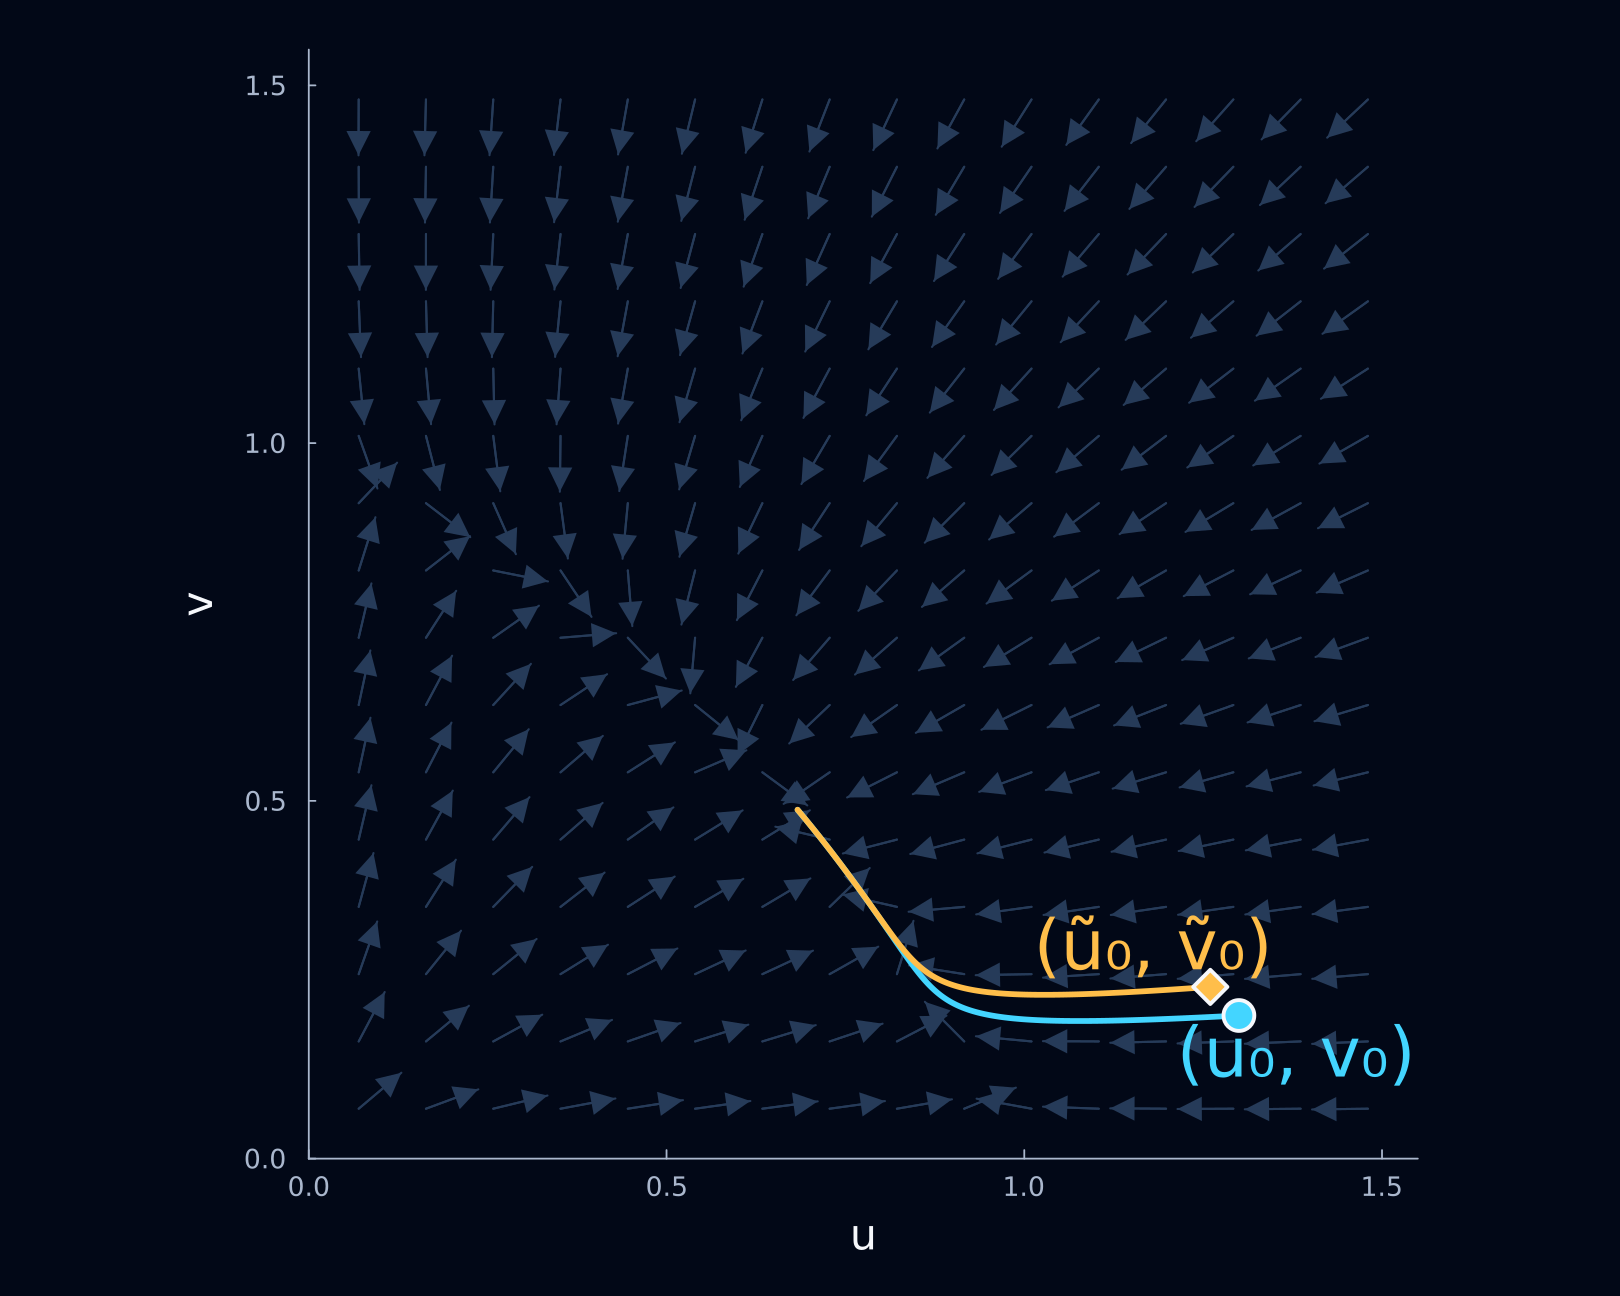
\includegraphics[
              width=\linewidth,
              height=3.80cm,
              keepaspectratio
            ]{figures/local_dynamics/stability_converging.png}

            \vspace{0.12cm}

            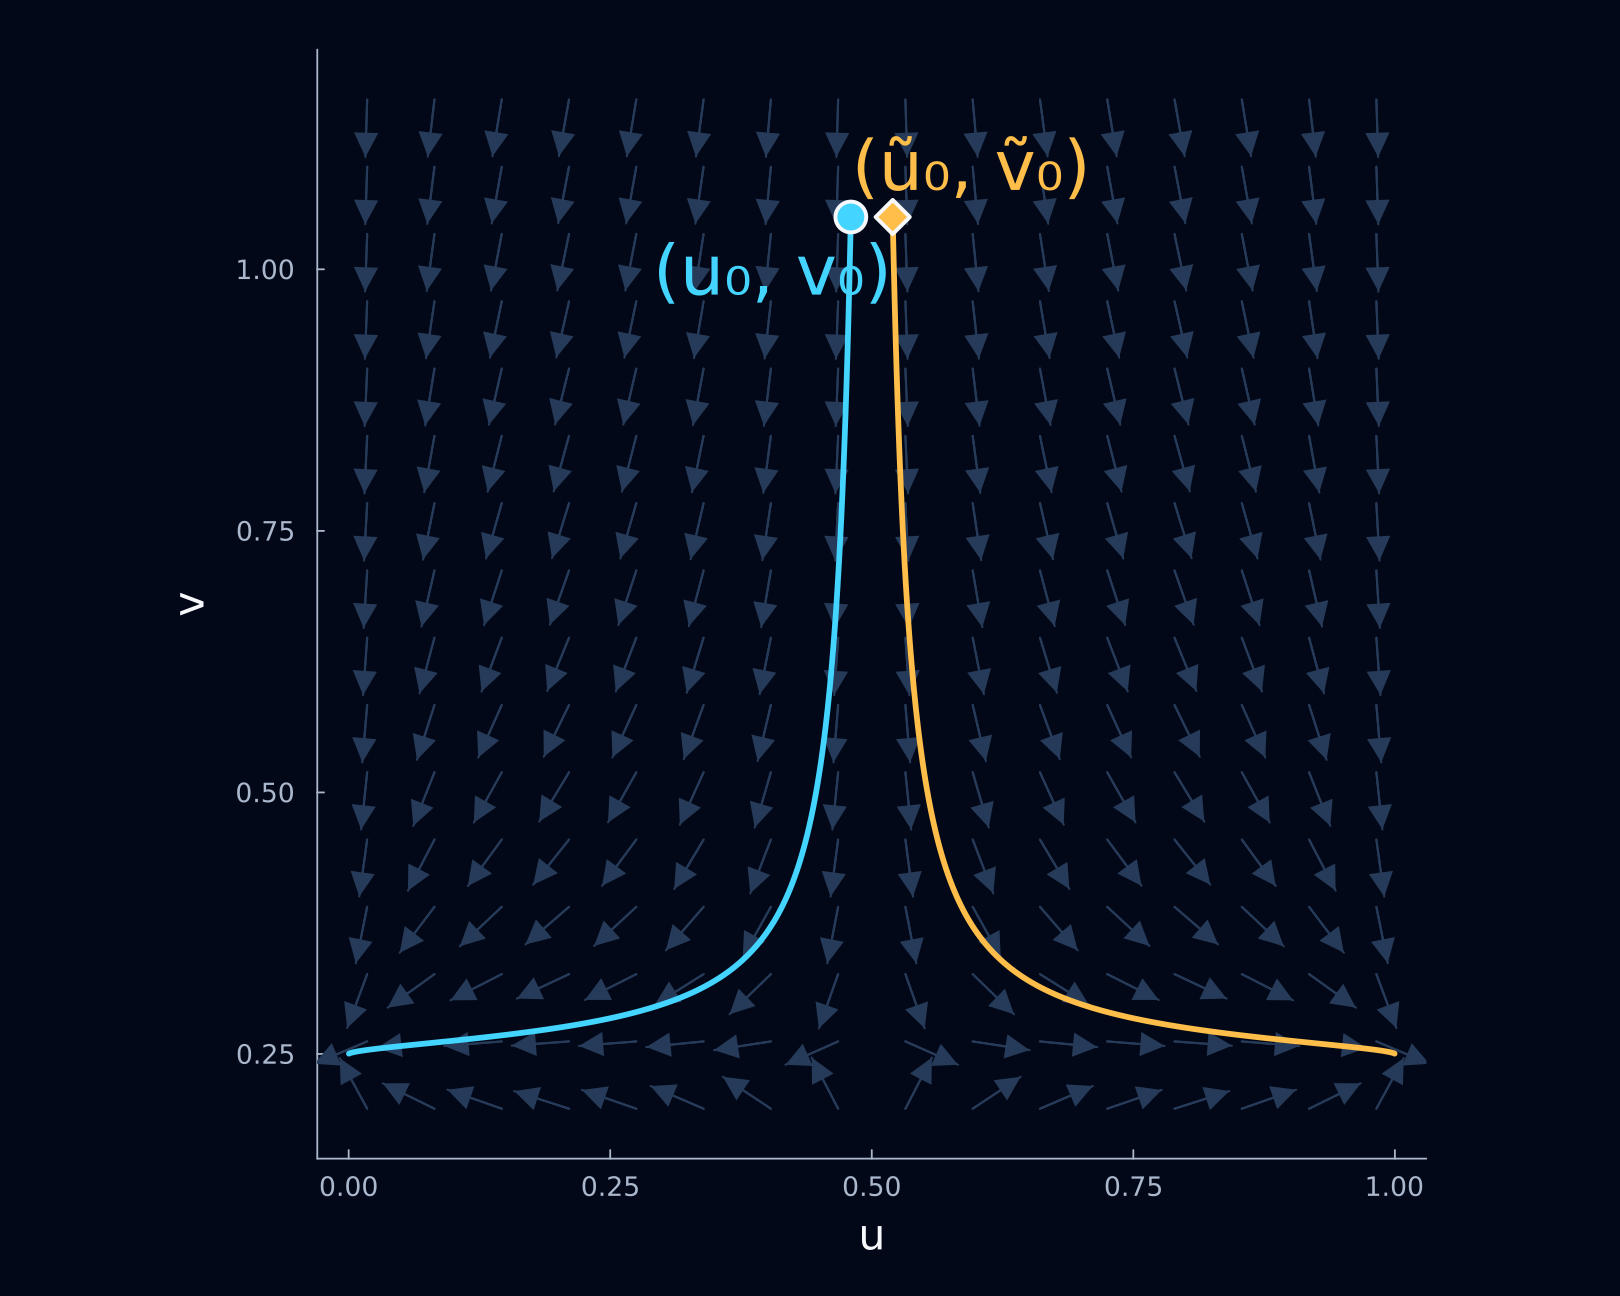
\includegraphics[
              width=\linewidth,
              height=3.80cm,
              keepaspectratio
            ]{figures/local_dynamics/stability_diverging.png}
          \end{column}

          \begin{column}{0.25\linewidth}

            \begin{minipage}[c][2.80cm][c]{\linewidth}
              {\color{HydraCyan}\bfseries
                \fontsize{7.7}{9.2}\selectfont
                STABLE
              \par}

              \vspace{0.08cm}

              {\color{HydraMuted}
                \fontsize{7.2}{9}\selectfont
                Nearby solutions converge
              \par}
            \end{minipage}

            \vspace{0.12cm}

            \begin{minipage}[c][2.80cm][c]{\linewidth}
              {\color{HydraGold}\bfseries
                \fontsize{7.7}{9.2}\selectfont
                UNSTABLE
              \par}

              \vspace{0.08cm}

              {\color{HydraMuted}
                \fontsize{7.2}{9}\selectfont
                Nearby solutions separate
              \par}
            \end{minipage}

          \end{column}

        \end{columns}


    \end{column}

  \end{columns}

\end{frame}

\begin{frame}{Stability of constant steady state}

\vspace{-0.75cm}

\begin{columns}[c,onlytextwidth]

  \begin{column}{0.45\textwidth}

      {\color{HydraWhite}\fontsize{11.4}{14.6}\selectfont
      \begin{align*}
        u(0)&=\bar u+\eta_0
        \\
        v(0)&=\bar v+\xi_0
      \end{align*}
      }

      \vspace{-0.52cm}

      {\color{HydraMuted}\fontsize{7.8}{9.6}\selectfont
        The perturbation is given by
      \par}

      \vspace{-0.68cm}

      {\color{HydraWhite}\fontsize{11.4}{14.6}\selectfont
      \begin{align*}
        \eta(t)&=u(t)-\bar u
        \\
        \xi(t)&=v(t)-\bar v
      \end{align*}
      }

      \vspace{-0.58cm}

      \HydraPoint[HydraCyan]
        {Asymptotically stable}
        {Every sufficiently small perturbation returns to the equilibrium.}

      \vspace{-0.46cm}

      {\color{HydraWhite}\fontsize{10.4}{13.2}\selectfont
      \begin{align*}
        \begin{aligned}
          \eta(t)&\longrightarrow0
          \\
          \xi(t)&\longrightarrow0
        \end{aligned}
        \qquad
        \text{as }t\longrightarrow\infty
      \end{align*}
      }

      \vspace{-0.36cm}

      \HydraPoint[HydraRed]
        {Unstable}
        {At least one arbitrarily small perturbation moves away.}

    \end{column}

  \begin{column}{0.51\textwidth}
    \centering

    % REPLACEABLE VISUAL
    % Replace the tikzpicture with:
    % \includegraphics[width=\linewidth,height=5.25cm,keepaspectratio]{figures/local_dynamics/...}
    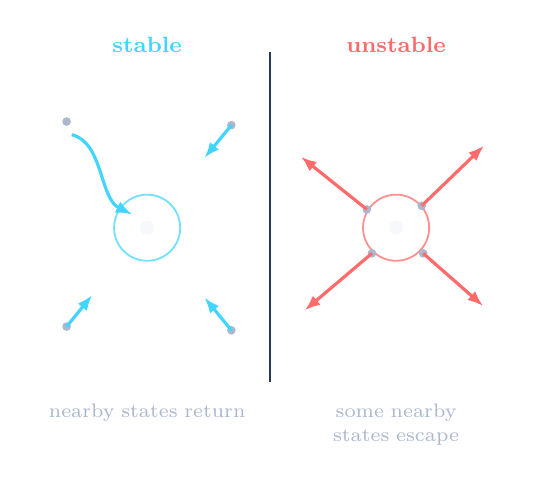
\begin{tikzpicture}[x=0.93cm,y=0.93cm]
      \node[text=HydraCyan,font=\bfseries\fontsize{8}{9.5}\selectfont]
        at (1.75,5.15) {stable};
      \node[text=HydraRed,font=\bfseries\fontsize{8}{9.5}\selectfont]
        at (5.15,5.15) {unstable};

      \draw[HydraLine,line width=0.75pt]
        (3.43,0.55) -- (3.43,5.05);

      \fill[HydraWhite]
        (1.75,2.65) circle[radius=0.09cm];

      \draw[HydraCyan,line width=0.65pt,opacity=0.75]
        (1.75,2.65) circle[radius=0.42cm];

      \fill[HydraMuted]
      (0.65,4.10) circle[radius=0.055cm];

      \foreach \x/\y in {
        % 0.65/4.10,
        0.65/1.30,
        2.90/4.05,
        2.90/1.25
      }{
        \fill[HydraMuted]
          (\x,\y) circle[radius=0.055cm];

        \draw[-{Latex[length=2mm]},HydraCyan,line width=1.15pt]
          (\x,\y) -- ($(1.75,2.65)!0.68!(\x,\y)$);
      }

      \draw[-{Latex[length=2.1mm]},HydraCyan,line width=1.15pt]
        (0.72,3.92)
        .. controls (1.15,3.82) and (1.10,3.05)
        .. (1.55,2.83);

      \fill[HydraWhite]
        (5.15,2.65) circle[radius=0.09cm];

      \draw[HydraRed,line width=0.65pt,opacity=0.75]
        (5.15,2.65) circle[radius=0.42cm];

      \foreach \x/\y/\dx/\dy in {
        4.75/2.90/-0.90/0.72,
        4.82/2.30/-0.92/-0.78,
        5.50/2.95/0.85/0.82,
        5.52/2.30/0.82/-0.72
      }{
        \fill[HydraMuted]
          (\x,\y) circle[radius=0.055cm];

        \draw[-{Latex[length=2mm]},HydraRed,line width=1.15pt]
          (\x,\y) -- ++(\dx,\dy);
      }

      \node[
        anchor=north,
        text=HydraMuted,
        text width=2.8cm,
        align=center,
        font=\fontsize{7.1}{8.6}\selectfont
      ] at (1.75,0.38)
        {nearby states return};

      \node[
        anchor=north,
        text=HydraMuted,
        text width=2.8cm,
        align=center,
        font=\fontsize{7.1}{8.6}\selectfont
      ] at (5.15,0.38)
        {some nearby states escape};
    \end{tikzpicture}

  \end{column}

\end{columns}

\end{frame}


\begin{frame}{Linearized stability}

  \vspace{-0.22cm}

  {\color{HydraMuted}\fontsize{7.9}{9.6}\selectfont
    Near the steady state $(\bar u,\bar v)$ write
  \par}

  \vspace{-0.40cm}

  {\color{HydraWhite}\fontsize{10.2}{13}\selectfont
  \begin{align*}
    u=\bar u+\eta, \quad 
    v=\bar v+\xi
  \end{align*}
  }

  \vspace{-0.52cm}

  \begin{columns}[T,onlytextwidth]

    \begin{column}{0.62\textwidth}
      {\color{HydraGold}\bfseries\fontsize{7.7}{9.2}\selectfont
        TAYLOR EXPANSION\par}

      \vspace{-0.24cm}

      {\color{HydraWhite}\fontsize{8.6}{10.8}\selectfont
      \begin{align*}
        \partial_t \eta
        &=
        f(\bar u+\eta,\bar v+\xi)=f(\bar u,\bar v)
        +
        f_u(\bar u,\bar v)\eta
        +
        f_v(\bar u,\bar v)\xi
        +
        O\!\left(\lVert(\eta,\xi)\rVert^2\right) \\
        \partial_t \xi
        &=
        g(\bar u+\eta,\bar v+\xi)=g(\bar u,\bar v)
        +
        g_u(\bar u,\bar v)\eta
        +
        g_v(\bar u,\bar v)\xi
        +
        O\!\left(\lVert(\eta,\xi)\rVert^2\right)
      \end{align*}
      }

    \end{column}

    \begin{column}{0.34\textwidth}
      {\color{HydraGold}\bfseries\fontsize{7.7}{9.2}\selectfont
        \centering JACOBIAN\par}

      \vspace{-0.26cm}

    {\color{HydraWhite}\fontsize{10.2}{13}\selectfont
    \begin{align*}
      \boxed{
        J(\bar u,\bar v)
        =
        \begin{pmatrix}
          f_u(\bar u,\bar v) & f_v(\bar u,\bar v)
          \\
          g_u(\bar u,\bar v) & g_v(\bar u,\bar v)
        \end{pmatrix}
      }
    \end{align*}
    }


    \end{column}

  \end{columns}

  \vspace{-0.12cm}

  {\color{HydraGold}\bfseries\fontsize{7.7}{9.2}\selectfont
    NEGLECTING HIGHER-ORDER TERMS\par}

  \vspace{-0.32cm}

  {\color{HydraWhite}\bfseries\fontsize{12.8}{16}\selectfont
  \begin{align*}
    \boxed{
      \begin{pmatrix}
        \partial_t \eta
        \\
        \partial_t \xi
      \end{pmatrix}
      =
      J(\bar u,\bar v)
      \begin{pmatrix}
        \eta
        \\
        \xi
      \end{pmatrix}
    }
  \end{align*}
  }

  \vspace{-0.30cm}

  \HydraTakeaway{
    Close to the steady state, the Jacobian determines the leading-order dynamics
  }

\end{frame}


\begin{frame}{Eigenvalues of the Jacobian}

\vspace{-0.38cm}

\begin{columns}[c,onlytextwidth]

  \begin{column}{0.47\textwidth}
    \centering

    {\color{HydraGold}\bfseries\fontsize{8}{9.6}\selectfont
      LINEARIZED SYSTEM
    \par}

    \vspace{-0.20cm}

    {\color{HydraWhite}\fontsize{10.2}{13}\selectfont
    \begin{align*}
      \begin{pmatrix}
        \partial_t\eta
        \\
        \partial_t\xi
      \end{pmatrix}
      =
      J(\bar u,\bar v)
      \begin{pmatrix}
        \eta
        \\
        \xi
      \end{pmatrix}
    \end{align*}
    }
  \end{column}

  \begin{column}{0.49\textwidth}
    \centering

    % {\color{HydraGold}\bfseries\fontsize{8}{9.6}\selectfont
    %   JACOBIAN
    % \par}

    \vspace{-0.20cm}

    {\color{HydraWhite}\fontsize{9.2}{11.8}\selectfont
    \begin{align*}
      J(\bar u,\bar v)
      =
      \begin{pmatrix}
        f_u(\bar u,\bar v) & f_v(\bar u,\bar v)
        \\
        g_u(\bar u,\bar v) & g_v(\bar u,\bar v)
      \end{pmatrix}
    \end{align*}
    }

    \vspace{-0.34cm}

    {\color{HydraMuted}\fontsize{7.5}{9.2}\selectfont
      The eigenvalues are the roots of
    \par}

    \vspace{-0.28cm}

    {\color{HydraWhite}\fontsize{9.4}{12}\selectfont
    \begin{align*}
      \det\!\left(
        J(\bar u,\bar v)-\lambda I
      \right)=0
    \end{align*}
    }
  \end{column}

\end{columns}

\vspace{-0.32cm}

\begin{center}
  \begin{minipage}{0.90\textwidth}

    {\color{HydraGold}\bfseries\fontsize{9.2}{11}\selectfont
      THEOREM
    \par}

    \vspace{0.12cm}

    {\color{HydraWhite}\fontsize{8.4}{10.5}\selectfont
      Let $\lambda_1$ and $\lambda_2$ be the eigenvalues of
      $J(\bar u,\bar v)$
    \par}

    \vspace{0.18cm}

    {\color{HydraBody}\fontsize{8.6}{10.8}\selectfont
    \begin{itemize}
      \setlength{\itemsep}{0.28cm}

      \item
        If
        $\operatorname{Re}\lambda_1<0$
        and
        $\operatorname{Re}\lambda_2<0$
        then the steady state $(\bar u,\bar v)$ is
        \textcolor{HydraCyan}{\bfseries asymptotically stable}

      \item
        If
        $\operatorname{Re}\lambda_i>0$
        for at least one eigenvalue then the steady state
        $(\bar u,\bar v)$ is
        \textcolor{HydraRed}{\bfseries unstable}

    \end{itemize}
    }

    \vspace{0.12cm}

    {\color{HydraMuted}\fontsize{7.2}{8.8}\selectfont
      If an eigenvalue has zero real part, linearization alone may be inconclusive
    \par}

  \end{minipage}
\end{center}

\end{frame}


\begin{frame}{Eigenvalues}

\vspace{-0.48cm}

\begin{columns}[c,onlytextwidth]

  \begin{column}{0.43\textwidth}
    \centering

    \vspace{-0.24cm}

    {\color{HydraWhite}\fontsize{9.4}{12}\selectfont
    \begin{align*}
      \begin{pmatrix}
        \partial_t\eta
        \\
        \partial_t\xi
      \end{pmatrix}
      =
      J(\bar u,\bar v)
      \begin{pmatrix}
        \eta
        \\
        \xi
      \end{pmatrix}
    \end{align*}
    }
  \end{column}

  \begin{column}{0.53\textwidth}
    \centering


    \vspace{-0.24cm}

    {\color{HydraWhite}\fontsize{8.8}{11.2}\selectfont
    \begin{align*}
      J(\bar u,\bar v)
      =
      \begin{pmatrix}
        f_u(\bar u,\bar v) & f_v(\bar u,\bar v)
        \\
        g_u(\bar u,\bar v) & g_v(\bar u,\bar v)
      \end{pmatrix}
    \end{align*}
    }
  \end{column}

\end{columns}

\vspace{-0.38cm}

\begin{center}
  {\color{HydraGold}\bfseries\fontsize{7.8}{9.4}\selectfont
    CHARACTERISTIC EQUATION
  \par}

  \vspace{-0.24cm}

  {\color{HydraWhite}\fontsize{8.8}{11.2}\selectfont
  \begin{align*}
    \det\!\left(J-\lambda I\right)=
    \begin{vmatrix}
      f_u-\lambda & f_v
      \\
      g_u & g_v-\lambda
    \end{vmatrix}
    =
    (f_u-\lambda)(g_v-\lambda)-f_vg_u=
    \lambda^2-\operatorname{tr}(J)\lambda+\det(J)
  \end{align*}
  }
\end{center}
 
\vspace{-0.34cm}

\begin{columns}[t,onlytextwidth]

  \begin{column}{0.47\textwidth}

    {\color{HydraGold}\bfseries\fontsize{8.4}{10}\selectfont
      DETERMINANT
    \par}

    \vspace{0.10cm}

    {\color{HydraBody}\fontsize{7.8}{9.7}\selectfont
    \begin{itemize}
      \setlength{\itemsep}{0.20cm}

      \item
        If $\det(J)<0$, one eigenvalue is positive and one is negative

        \textcolor{HydraRed}{\bfseries The steady state is an unstable saddle}

      \item
        If $\det(J)>0$, real eigenvalues have the same sign or form a complex conjugate pair

        \textcolor{HydraMuted}{The trace determines the sign of their real parts}

    \end{itemize}
    }

  \end{column}

  \begin{column}{0.47\textwidth}

    {\color{HydraGold}\bfseries\fontsize{8.4}{10}\selectfont
      TRACE WHEN $\det(J)>0$
    \par}

    \vspace{0.10cm}

    {\color{HydraBody}\fontsize{7.8}{9.7}\selectfont
    \begin{itemize}
      \setlength{\itemsep}{0.20cm}

      \item
        If $\operatorname{tr}(J)<0$, both eigenvalues have negative real parts

        \textcolor{HydraCyan}{\bfseries The steady state is asymptotically stable}

      \item
        If $\operatorname{tr}(J)>0$, both eigenvalues have positive real parts

        \textcolor{HydraRed}{\bfseries The steady state is unstable}

    \end{itemize}
    }

  \end{column}

\end{columns}

\vspace{0.10cm}

\end{frame}

\begin{frame}{Eigenvalues determine local stability}

\vspace{-0.35cm}

\begin{center}
  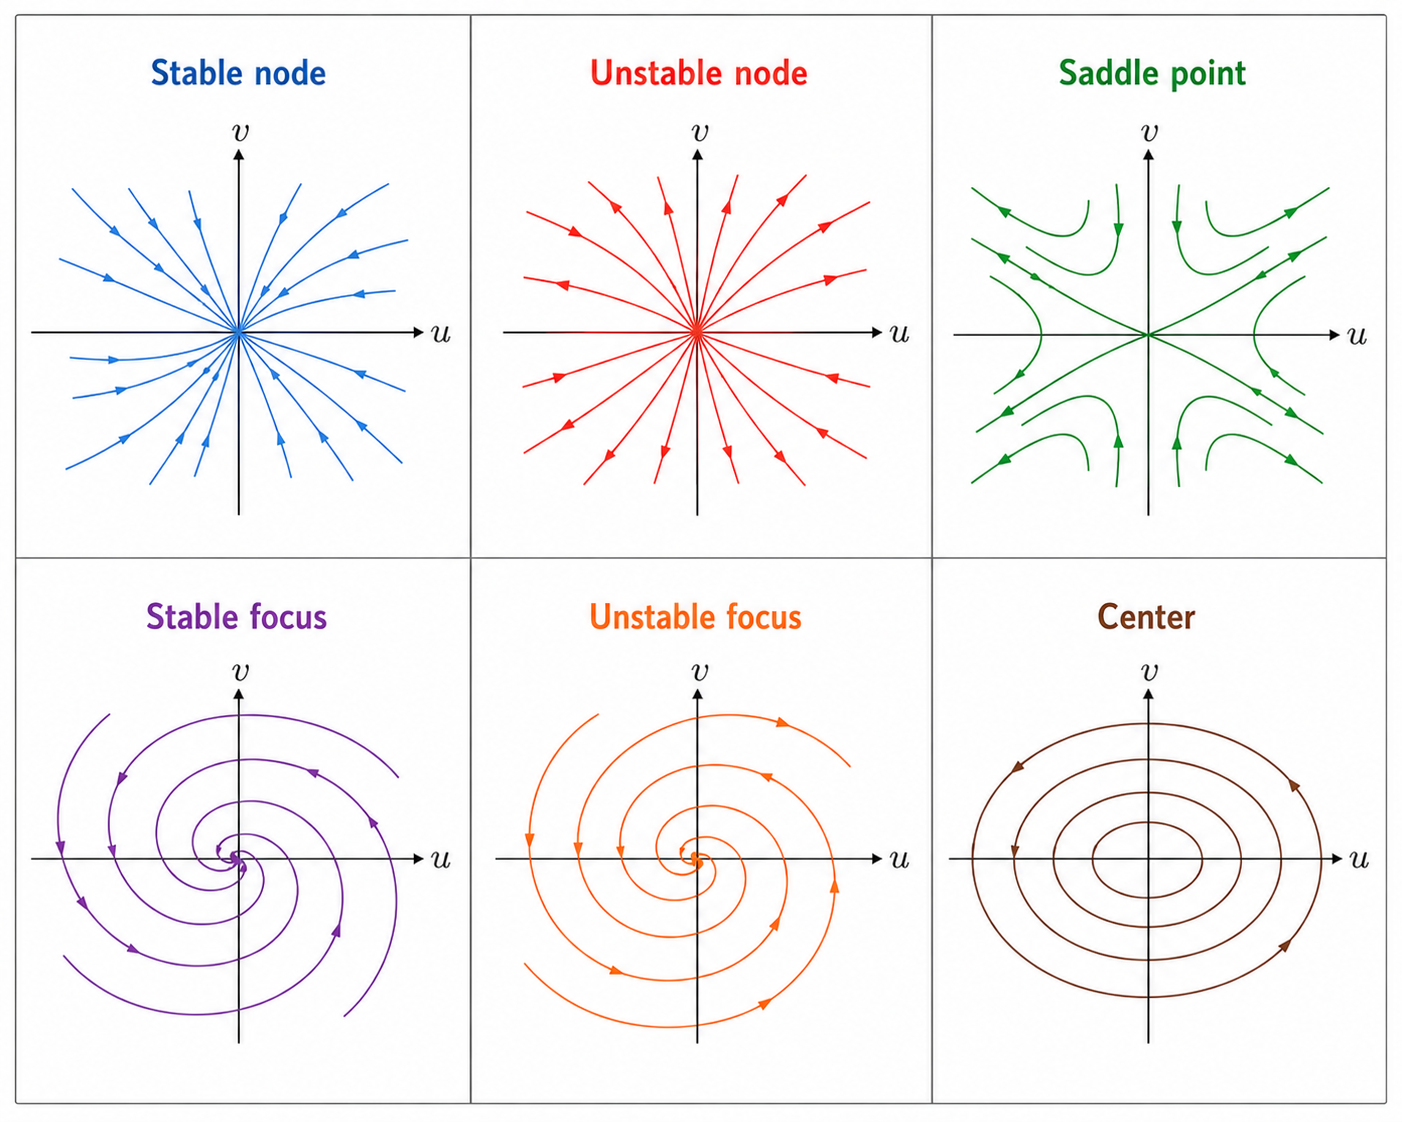
\includegraphics[
    width=0.98\textwidth,
    height=6.75cm,
    keepaspectratio
  ]{figures/local_dynamics/EigenvalueNode.png}
\end{center}

\end{frame}


\begin{frame}{Trace and determinant classify a two-variable equilibrium}

\vspace{-0.12cm}

\begin{columns}[c,onlytextwidth]

\begin{column}{0.46\textwidth}

  {\color{HydraWhite}\fontsize{9.6}{12.2}\selectfont
  \begin{align*}
    \det\!\left(
      J(\bar u,\bar v)-\lambda I
    \right)&=0
    \end{align*}
    \begin{align*}
    \boxed{
      \lambda^2
      -\operatorname{tr}(J)\lambda
      +\det(J)
      =0
    }
  \end{align*}
  }

  \vspace{-0.028cm}

  {\color{HydraMuted}\fontsize{7.8}{9.6}\selectfont
    Therefore
  \par}

  \vspace{-0.26cm}

  {\color{HydraWhite}\fontsize{9.6}{12.2}\selectfont
  \begin{align*}
    \lambda_1+\lambda_2
    &=
    \operatorname{tr}(J)
    \\
    \lambda_1\lambda_2
    &=
    \det(J)
  \end{align*}
  }



\end{column}

\begin{column}{0.50\textwidth}
  \centering

  % REPLACEABLE VISUAL
  % Replace the tikzpicture with:
  % \includegraphics[width=\linewidth,height=5.45cm,keepaspectratio]
  % {figures/local_dynamics/...}
  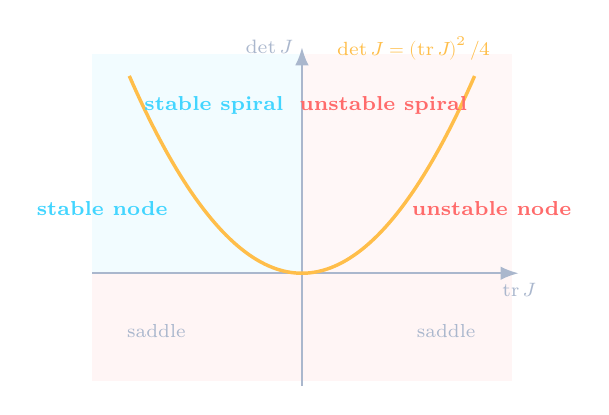
\begin{tikzpicture}[x=0.86cm,y=0.82cm]

    \fill[HydraRed,opacity=0.07]
      (0.35,0.48) rectangle (6.55,2.15);

    \fill[HydraCyan,opacity=0.07]
      (0.35,2.15) rectangle (3.45,5.55);

    \fill[HydraRed,opacity=0.05]
      (3.45,2.15) rectangle (6.55,5.55);

    \draw[-{Latex[length=2.3mm]},HydraMuted,line width=0.75pt]
      (0.35,2.15) -- (6.65,2.15)
      node[below,text=HydraMuted,
        font=\fontsize{7}{8.2}\selectfont]
      {$\operatorname{tr}J$};

    \draw[-{Latex[length=2.3mm]},HydraMuted,line width=0.75pt]
      (3.45,0.40) -- (3.45,5.65)
      node[left,text=HydraMuted,
        font=\fontsize{7}{8.2}\selectfont]
      {$\det J$};

    \draw[
      HydraGold,
      line width=1.25pt,
      domain=-2.55:2.55,
      samples=90
    ]
      plot ({3.45+\x},{2.15+0.47*\x*\x});

    \node[
      text=HydraMuted,
      font=\fontsize{6.8}{8.2}\selectfont
    ]
      at (1.30,1.25) {saddle};

    \node[
      text=HydraMuted,
      font=\fontsize{6.8}{8.2}\selectfont
    ]
      at (5.58,1.25) {saddle};

    \node[
      text=HydraCyan,
      font=\bfseries\fontsize{7.3}{8.8}\selectfont
    ]
      at (0.5,3.15) {stable node};

    \node[
      text=HydraCyan,
      font=\bfseries\fontsize{7.3}{8.8}\selectfont
    ]
      at (2.15,4.75) {stable spiral};

    \node[
      text=HydraRed,
      font=\bfseries\fontsize{7.3}{8.8}\selectfont
    ]
      at (6.25,3.15) {unstable node};

    \node[
      text=HydraRed,
      font=\bfseries\fontsize{7.3}{8.8}\selectfont
    ]
      at (4.65,4.75) {unstable spiral};

    \node[
      anchor=south east,
      text=HydraGold,
      font=\fontsize{6.9}{8.3}\selectfont
    ]
      at (6.38,5.30)
      {$\det J=\left(\operatorname{tr}J\right)^2/4$};

  \end{tikzpicture}

\end{column}

\end{columns}

\end{frame}




% \begin{frame}{Turing instability begins with a locally stable equilibrium}

%   \vspace{-0.05cm}

%   \begin{columns}[c,onlytextwidth]

%     \begin{column}{0.43\textwidth}
%       {\color{HydraGold}\bfseries\fontsize{7.8}{9.4}\selectfont
%         REACTIONS ALONE\par}

%       \vspace{-0.12cm}

%       {\color{HydraWhite}\fontsize{11.4}{14.4}\selectfont
%       \[
%         \dot{\boldsymbol\eta}=J_*\boldsymbol\eta
%       \]
%       }

%       \vspace{-0.22cm}

%       {\color{HydraWhite}\fontsize{10.8}{13.6}\selectfont
%       \[
%         \operatorname{tr}J_*<0
%         \qquad
%         \det J_*>0
%       \]
%       }

%       \vspace{-0.12cm}

%       \HydraPoint[HydraCyan]
%         {Homogeneous perturbations decay}
%         {If every point is perturbed in the same way, the local kinetics restore the equilibrium.}

%       \vspace{-0.24cm}

%       {\color{HydraMuted}\fontsize{7.8}{9.6}\selectfont
%         This stability is essential: the pattern must be created by spatial coupling, not by unstable reactions.
%       \par}
%     \end{column}

%     \begin{column}{0.53\textwidth}
%       {\color{HydraGold}\bfseries\fontsize{7.8}{9.4}\selectfont
%         ADD DIFFUSION\par}

%       \vspace{-0.14cm}

%       {\color{HydraWhite}\fontsize{11.4}{14.4}\selectfont
%       \[
%         \partial_t\boldsymbol\eta
%         =
%         J_*\boldsymbol\eta
%         +
%         \mathcal D\Delta\boldsymbol\eta
%       \]
%       }

%       \vspace{-0.24cm}

%       \centering

%       % REPLACEABLE VISUAL
%       % Replace the tikzpicture with:
%       % \includegraphics[width=\linewidth,height=2.75cm,keepaspectratio]{figures/local_dynamics/...}
%       \begin{tikzpicture}[x=0.96cm,y=0.96cm]
%         \draw[-{Latex[length=2.2mm]},HydraMuted,line width=0.75pt]
%           (0.35,0.55) -- (7.10,0.55)
%           node[below,text=HydraMuted,font=\fontsize{7}{8.2}\selectfont] {$x$};
%         \draw[HydraLine,line width=0.70pt] (0.45,2.10) -- (6.85,2.10);
%         \draw[HydraCyan,line width=1.55pt,domain=0.45:6.85,samples=100]
%           plot (\x,{2.10+0.55*cos(180*3*(\x-0.45)/6.40)});

%         \foreach \x in {0.55,1.25,...,6.85}{
%           \fill[HydraWhite,opacity=0.75] (\x,2.10) circle[radius=0.045cm];
%         }

%         \node[anchor=south west,text=HydraCyan,
%           font=\bfseries\fontsize{7.5}{9}\selectfont]
%           at (0.55,2.82) {nonconstant spatial perturbation};
%         \node[anchor=north,text=HydraMuted,text width=6.4cm,align=center,
%           font=\fontsize{7.1}{8.6}\selectfont]
%           at (3.65,0.16)
%           {different spatial modes will be tested separately};
%       \end{tikzpicture}

%       \vspace{-0.10cm}

%       {\color{HydraWhite}\bfseries\fontsize{9.6}{12}\selectfont
%         Can diffusion destabilize one nonconstant mode?
%       \par}
%     \end{column}

%   \end{columns}

%   \vspace{0.12cm}

%   \HydraTakeaway{
%     Turing instability is diffusion-driven loss of stability.
%   }

% \end{frame}

\HydraSection[
  focus x=0.62,
  focus y=0.34,
  radius=0.12,
  zoom=1.95
]{Turing instability}

\HydraSubsection[
  \mbox{Two interacting substances can turn}
  \mbox{diffusion from a smoothing process}
  \mbox{into a source of spatial structure}
]{The Turing idea}

\begin{frame}{Scalar reaction--diffusion equation}

\vspace{-0.40cm}

\begin{columns}[c,onlytextwidth]

\begin{column}{0.57\textwidth}

  {\color{HydraWhite}\fontsize{11.2}{14.2}\selectfont
  \begin{align*}
    \partial_tu=D\Delta u+f(u)
  \end{align*}
  }

  \vspace{-0.42cm}

  {\color{HydraMuted}\fontsize{7.8}{9.6}\selectfont
    Let $\bar u$ be a stable homogeneous equilibrium
  \par}

  \vspace{-0.40cm}

  {\color{HydraWhite}\fontsize{10.4}{13.2}\selectfont
  \begin{align*}
    f(\bar u)&=0
    \qquad
    f'(\bar u)<0
  \end{align*}
  }

  \vspace{-0.44cm}

  {\color{HydraMuted}\fontsize{7.8}{9.6}\selectfont
    For a perturbation in the $k$th spatial eigenfunction
  \par}

  \vspace{-0.38cm}

  {\color{HydraWhite}\fontsize{10.2}{13}\selectfont
  \begin{align*}
    u(x,t)
    &=
    \bar u+a_k(t)\phi_k(x)
    \\
    \partial_ta_k
    &=
    \left(f'(\bar u)-D\mu_k\right)a_k
  \end{align*}
  }

  \vspace{-0.50cm}

  {\color{HydraWhite}\bfseries\fontsize{13.4}{16.4}\selectfont
  \begin{align*}
    \boxed{
      \lambda_k=f'(\bar u)-D\mu_k<0
    }
  \end{align*}
  }

\end{column}

\begin{column}{0.39\textwidth}
  \centering

  % REPLACEABLE VISUAL
  % Replace the tikzpicture with:
  % \includegraphics[width=\linewidth,height=4.85cm,keepaspectratio]
  % {figures/turing/...}
  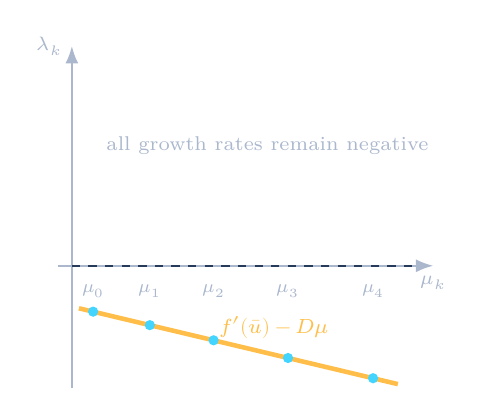
\begin{tikzpicture}[x=0.90cm,y=0.90cm]

    \draw[-{Latex[length=2.2mm]},HydraMuted,line width=0.75pt]
      (0.45,2.15) -- (5.75,2.15)
      node[
        below,
        text=HydraMuted,
        font=\fontsize{7}{8.2}\selectfont
      ]
      {$\mu_k$};

    \draw[-{Latex[length=2.2mm]},HydraMuted,line width=0.75pt]
      (0.65,0.42) -- (0.65,5.25)
      node[
        left,
        text=HydraMuted,
        font=\fontsize{7}{8.2}\selectfont
      ]
      {$\lambda_k$};

    \draw[HydraGold,line width=1.65pt]
      (0.75,1.55) -- (5.25,0.48);

    \foreach \x/\lab in {
      0.95/0,
      1.75/1,
      2.65/2,
      3.70/3,
      4.90/4
    }{
      \pgfmathsetmacro{\yy}{1.55-0.2378*(\x-0.75)}

      \fill[HydraCyan]
        (\x,\yy) circle[radius=0.065cm];

      \node[
        anchor=north,
        text=HydraMuted,
        font=\fontsize{6.5}{7.8}\selectfont
      ]
        at (\x,2.02)
        {$\mu_{\lab}$};
    }

    \node[
      anchor=west,
      text=HydraGold,
      font=\bfseries\fontsize{7.4}{8.9}\selectfont
    ]
      at (2.60,1.28)
      {$f'(\bar u)-D\mu$};

    \node[
      anchor=west,
      text=HydraMuted,
      font=\fontsize{7.2}{8.7}\selectfont
    ]
      at (1.00,3.85)
      {all growth rates remain negative};

    \draw[dashed,HydraLine,line width=0.7pt]
      (0.65,2.15) -- (5.45,2.15);

  \end{tikzpicture}

  \vspace{-0.10cm}

  \HydraPoint[HydraCyan]
    {Diffusion adds damping}
    {Every nonconstant spatial mode is more stable than the homogeneous mode.}

\end{column}

\end{columns}

\end{frame}


\begin{frame}{Scalar reaction--diffusion equation: no stable patterns}

% \vspace{-0.42cm}

\begin{center}
  \begin{minipage}{0.88\textwidth}

    \vspace{-0.20cm}

    {\color{HydraWhite}\fontsize{9.8}{12.5}\selectfont
    \begin{align*}
      \partial_tu
      &=
      D\Delta u+f(u)
      &&
      x\in\Omega
      \quad
      t>0
      \\
      u(x,0)
      &=
      u_0(x)
      &&
      x\in\Omega
      \\
      \nabla u\cdot\mathbf n
      &=
      0
      &&
      x\in\partial\Omega
    \end{align*}
    }
  \end{minipage}
\end{center}

\vspace{0.58cm}

\begin{center}
  \begin{minipage}{0.88\textwidth}

    {\color{HydraGold}\bfseries\fontsize{9.2}{11}\selectfont
      THEOREM
    \par}

    \vspace{0.14cm}

    {\color{HydraWhite}\fontsize{9}{11.5}\selectfont
      Let $\Omega\subset\mathbb R^n$ be a bounded convex domain.
      Every nonconstant stationary solution of the scalar
      reaction--diffusion equation with homogeneous Neumann
      boundary conditions is unstable
    \par}

    \vspace{0.28cm}

    {\color{HydraCyan}\bfseries\fontsize{9.4}{12}\selectfont
      Every stable stationary solution is spatially constant
    \par}

    \vspace{-0.14cm}

    {\color{HydraWhite}\fontsize{10.4}{13.2}\selectfont
    \begin{align*}
      u(x)\equiv\bar u
      \qquad \text{and} \qquad
      f(\bar u)=0
    \end{align*}
    }

  \end{minipage}
\end{center}

\vfill

\HydraTakeaway{
  One diffusing substance cannot maintain a stable spatial pattern
}

\end{frame}




\begin{frame}{Diffusion-driven instability}

  \vspace{-0.08cm}

  \begin{columns}[c,onlytextwidth]

    \begin{column}{0.27\textwidth}
      \centering

      \includegraphics[
        width=0.78\linewidth,
        height=3.55cm,
        keepaspectratio
      ]{figures/hydra/Alan_Turing_(1951).jpg}

      \vspace{0.08cm}

      {\color{HydraGold}\bfseries\fontsize{18}{21}\selectfont
        1952\par}

      {\color{HydraWhite}\bfseries\fontsize{9.2}{11}\selectfont
        Alan Turing\par}

      \vspace{0.04cm}

      {\color{HydraMuted}\fontsize{6.6}{8.1}\selectfont
        \textit{The Chemical Basis of Morphogenesis}
      \par}
    \end{column}

    \begin{column}{0.67\textwidth}
      {\color{HydraWhite}\fontsize{12.6}{16}\selectfont
      \[
        \begin{aligned}
          \partial_tu&=D_u\Delta u+f(u,v)
          \\
          \partial_tv&=D_v\Delta v+g(u,v)
        \end{aligned}
      \]
      }

      \vspace{-0.10cm}

      \HydraPoint[HydraGold]
        {Stable reactions}
        {Without spatial transport, small perturbations return to the homogeneous equilibrium.}

      \vspace{0.32cm}

      \HydraPoint[HydraCyan]
        {Unstable reaction--diffusion system}
        {After diffusion is introduced, one nonconstant spatial mode can begin to grow.}

      \vspace{-0.20cm}

      {\color{HydraWhite}\bfseries\fontsize{13.2}{16.2}\selectfont
      \[
        \boxed{D_u\neq D_v}
      \]
      }

      \vspace{-0.24cm}

      {\color{HydraMuted}\fontsize{7.8}{9.5}\selectfont
        Unequal diffusion is essential for classical two-species Turing instability.
      \par}
    \end{column}

  \end{columns}

  \source{
    A.~M. Turing, \textit{Phil. Trans. R. Soc. B} 237 (1952), 37--72.
    Portrait: Elliott \& Fry, 1951, Wikimedia Commons.
  }

\end{frame}


\begin{frame}{Equal diffusion shifts every spatial mode toward stability}

  \vspace{-0.35cm}

  \begin{center}
    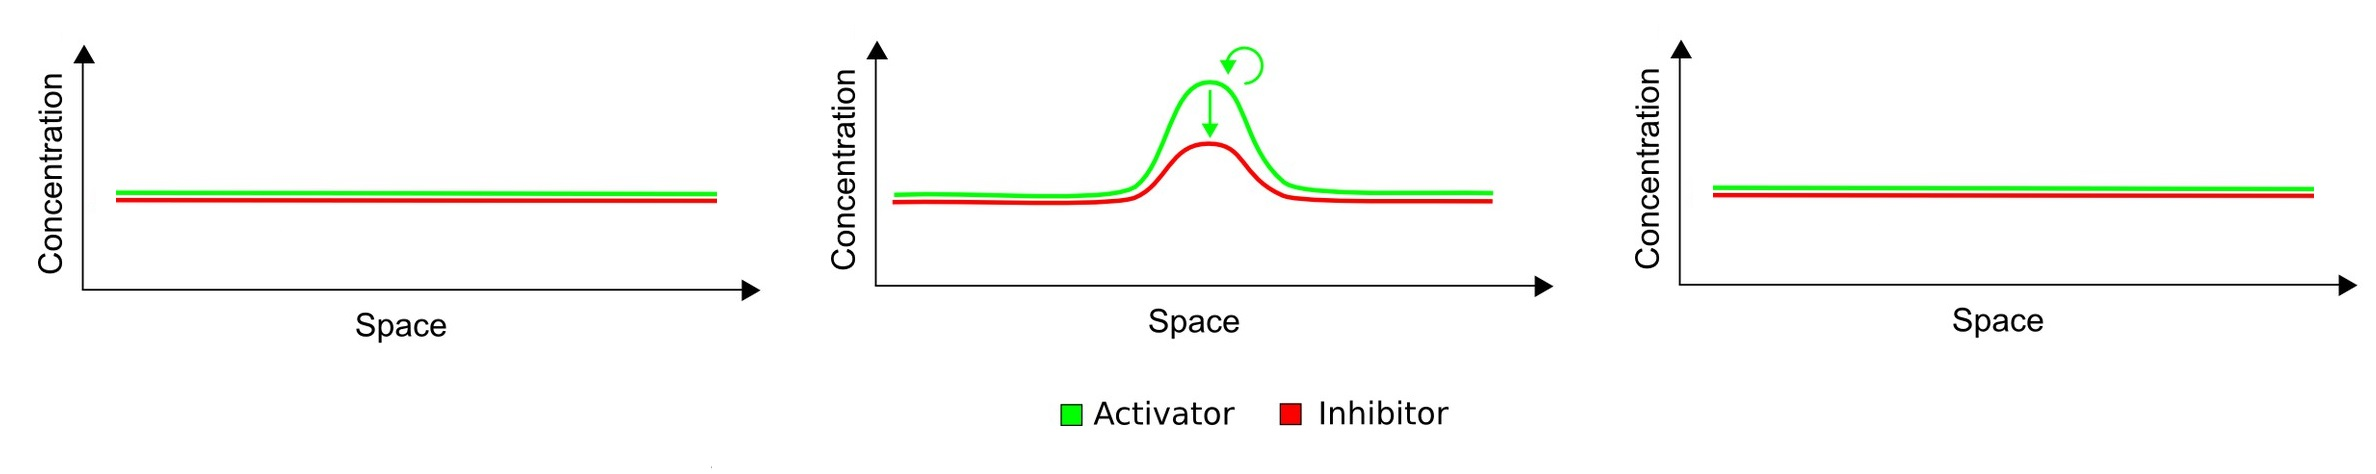
\includegraphics[
      width=0.98\textwidth,
      height=6.75cm,
      keepaspectratio
    ]{figures/turing/lax_14022_elife-14022-app3-fig1-v4.jpg}
  \end{center}

\end{frame}


\begin{frame}{Unequal diffusion can amplify a spatial mode}

  \vspace{-0.35cm}

  \begin{center}
    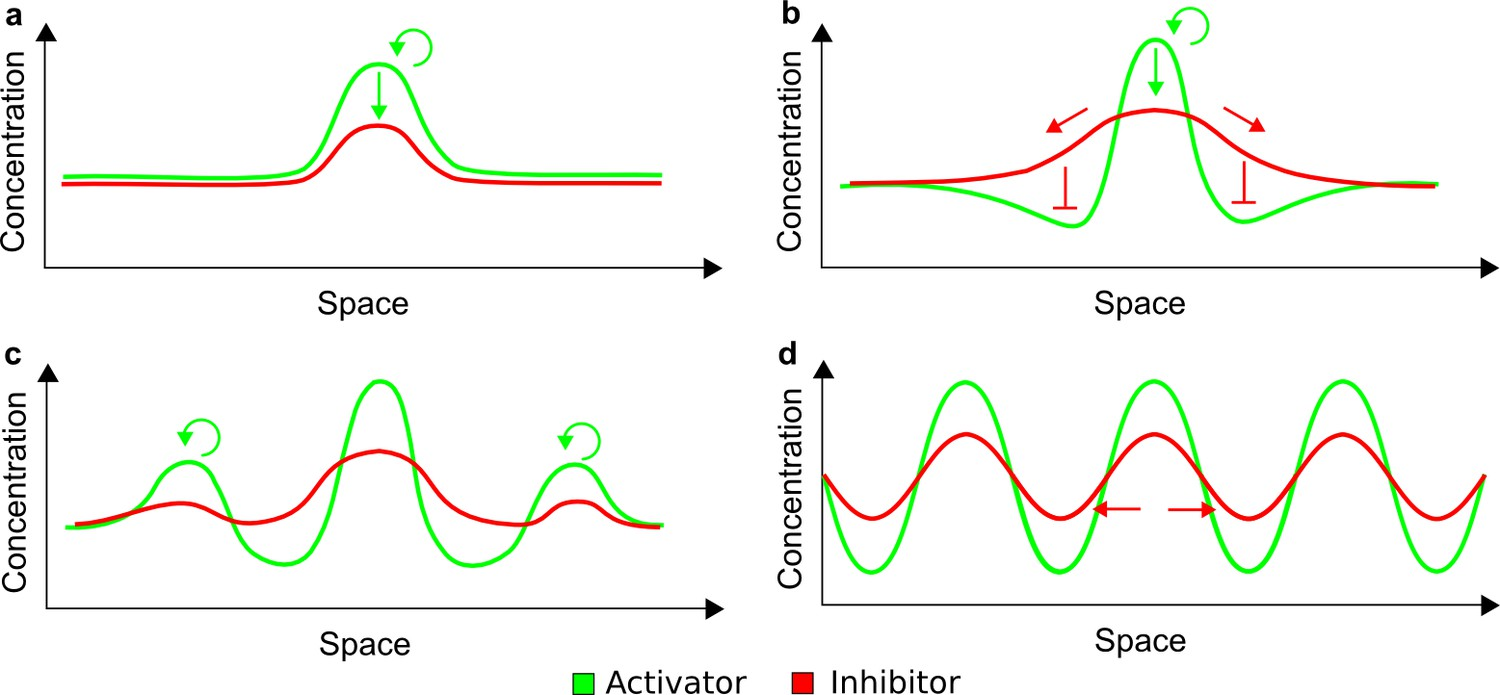
\includegraphics[
      width=0.98\textwidth,
      height=6.75cm,
      keepaspectratio
    ]{figures/turing/lax_14022_elife-14022-app3-fig1-v3.tif.jpg}
  \end{center}

\end{frame}





\HydraSubsection[
  \mbox{Linearization and spatial eigenfunctions}
  \mbox{reduce the PDE to one stability}
  \mbox{problem for each spatial mode}
]{Stability analysis}


\begin{frame}{The full reaction--diffusion problem}

  \vspace{-0.42cm}

  {\color{HydraWhite}\fontsize{8.4}{10.3}\selectfont
    Let $\Omega\subset\mathbb R^n$ be a bounded domain
  \par}

  \vspace{-0.26cm}

  {\color{HydraWhite}\fontsize{9.8}{12.4}\selectfont
  \begin{align*}
    \partial_tu
    &=D_u\Delta u+f(u,v)
    &&x\in\Omega
    \quad t>0
    \\
    \partial_tv
    &=D_v\Delta v+g(u,v)
    &&x\in\Omega
    \quad t>0
  \end{align*}
  }

  \vspace{0.16cm}

  {\color{HydraWhite}\fontsize{8.4}{10.3}\selectfont
    Initial conditions\par}

  \vspace{-0.28cm}

  {\color{HydraWhite}\fontsize{9.3}{11.7}\selectfont
  \begin{align*}
    u(x,0)&=u_0(x)
    &
    v(x,0)&=v_0(x)
    &&x\in\Omega
  \end{align*}
  }

  \vspace{-0.38cm}

  {\color{HydraWhite}\fontsize{8.4}{10.3}\selectfont
    Homogeneous Neumann boundary conditions\par}

  \vspace{-0.28cm}

  {\color{HydraWhite}\fontsize{9.3}{11.7}\selectfont
  \begin{align*}
    \nabla u\cdot\mathbf n
    &=0
    &
    \nabla v\cdot\mathbf n
    &=0
    &&x\in\partial\Omega
  \end{align*}
  }

  \vspace{-0.28cm}

  \begin{columns}[T,onlytextwidth]

    \begin{column}{0.56\textwidth}
      {\color{HydraGold}\fontsize{10}{10}\selectfont
        $\bullet$
      }
      {\color{HydraMuted}\fontsize{7.4}{9}\selectfont
        $f,g\in C^1(\mathbb R^2)$ describe local production,
        degradation and interactions at each spatial position
      }
    \end{column}

    \begin{column}{0.40\textwidth}
      {\color{HydraCyan}\fontsize{10}{10}\selectfont
        $\bullet$
      }
      {\color{HydraMuted}\fontsize{7.4}{9}\selectfont
        $D_u,D_v>0$ are the diffusion coefficients
      }
    \end{column}

  \end{columns}

\end{frame}


\begin{frame}{Homogeneous steady state}

  \vspace{-0.08cm}

  \begin{columns}[c,onlytextwidth]

    \begin{column}{0.58\textwidth}
      {\color{HydraGold}\bfseries\fontsize{7.6}{9.2}\selectfont
        HOMOGENEOUS EQUILIBRIUM\par}

      \vspace{-0.16cm}

      {\color{HydraWhite}\fontsize{11.6}{14.8}\selectfont
      \[
        \begin{pmatrix}
          u(x,t)\\
          v(x,t)
        \end{pmatrix}
        =
        \begin{pmatrix}
          \bar u\\
          \bar v
        \end{pmatrix}
      \]
      }

      \vspace{-0.22cm}

      {\color{HydraWhite}\fontsize{10.4}{13.2}\selectfont
      \[
        f(\bar u,\bar v)=0
        \qquad
        g(\bar u,\bar v)=0
      \]
      }

      \vspace{-0.18cm}

      {\color{HydraGold}\bfseries\fontsize{7.6}{9.2}\selectfont
        LOCAL JACOBIAN\par}

      \vspace{-0.16cm}

      {\color{HydraWhite}\fontsize{10.4}{13.2}\selectfont
      \[
        J(\bar u,\bar v)=
        \begin{pmatrix}
          f_u(\bar u,\bar v)&f_v(\bar u,\bar v)\\
          g_u(\bar u,\bar v)&g_v(\bar u,\bar v)
        \end{pmatrix}
      \]
      }

      \vspace{-0.08cm}

      {\color{HydraMuted}\fontsize{7.5}{9.1}\selectfont
        Both eigenvalues of $J(\bar u,\bar v)$ have negative real parts
      \par}

      \vspace{-0.18cm}

      {\color{HydraWhite}\bfseries\fontsize{11.6}{14.5}\selectfont
      \[
        \boxed{
          \operatorname{tr}J(\bar u,\bar v)<0
          \qquad
          \det J(\bar u,\bar v)>0
        }
      \]
      }
    \end{column}

    \begin{column}{0.38\textwidth}
      \centering

      % REPLACEABLE VISUAL
      % Replace the tikzpicture with:
      % \includegraphics[width=\linewidth,height=4.90cm,keepaspectratio]{figures/turing/...}
      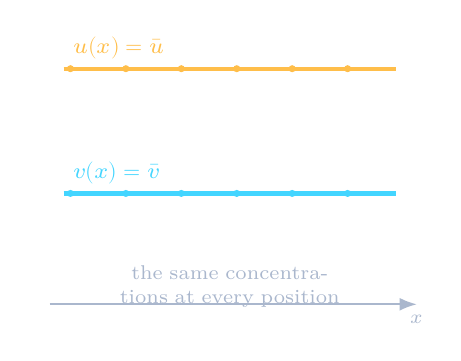
\begin{tikzpicture}[x=0.88cm,y=0.88cm]
        \draw[-{Latex[length=2.2mm]},HydraMuted,line width=0.75pt]
          (0.35,0.55) -- (5.65,0.55)
          node[below,text=HydraMuted,font=\fontsize{7}{8.2}\selectfont] {$x$};

        \draw[HydraGold,line width=1.55pt] (0.55,3.95) -- (5.35,3.95);
        \draw[HydraCyan,line width=1.55pt] (0.55,2.15) -- (5.35,2.15);

        \node[anchor=west,text=HydraGold,
          font=\bfseries\fontsize{8}{9.5}\selectfont]
          at (0.55,4.25) {$u(x)=\bar u$};
        \node[anchor=west,text=HydraCyan,
          font=\bfseries\fontsize{8}{9.5}\selectfont]
          at (0.55,2.45) {$v(x)=\bar v$};

        \foreach \x in {0.65,1.45,...,5.25}{
          \fill[HydraGold] (\x,3.95) circle[radius=0.045cm];
          \fill[HydraCyan] (\x,2.15) circle[radius=0.045cm];
        }

        \node[anchor=north,text=HydraMuted,text width=4.9cm,align=center,
          font=\fontsize{7.2}{8.8}\selectfont]
          at (2.95,1.25)
          {the same concentrations at every position};
      \end{tikzpicture}

      \vspace{-0.12cm}

      \HydraPoint[HydraCyan]
        {Stable without spatial variation}
        {The reaction kinetics restore every sufficiently small homogeneous perturbation.}
    \end{column}

  \end{columns}

\end{frame}


\begin{frame}{Perturb both concentrations around the steady state}

  \vspace{-0.44cm}

  \begin{columns}[T,onlytextwidth]

    \begin{column}{0.40\textwidth}
      {\color{HydraGold}\bfseries\fontsize{7.6}{9.2}\selectfont
        SMALL PERTURBATION\par}

      \vspace{-0.28cm}

      {\color{HydraWhite}\fontsize{9.5}{12}\selectfont
      \begin{align*}
        u(x,t)&=\bar u+\eta(x,t)
        \\
        v(x,t)&=\bar v+\xi(x,t)
      \end{align*}
      }

      \vspace{-0.42cm}

      % REPLACEABLE VISUAL
      % Replace the tikzpicture with:
      % \includegraphics[width=\linewidth,height=2.20cm,keepaspectratio]{figures/turing/...}
      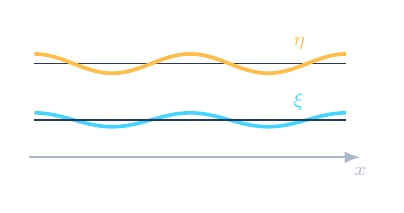
\begin{tikzpicture}[x=0.72cm,y=0.68cm]
        \draw[-{Latex[length=2mm]},HydraMuted,line width=0.7pt]
          (0.35,0.45) -- (6.20,0.45)
          node[below,text=HydraMuted,font=\fontsize{6.8}{8}\selectfont] {$x$};
        \draw[HydraLine,line width=0.65pt] (0.45,2.20) -- (5.95,2.20);
        \draw[HydraGold,line width=1.35pt,domain=0.45:5.95,samples=100]
          plot (\x,{2.20+0.18*cos(360*2*(\x-0.45)/5.50)});
        \draw[HydraCyan,line width=1.30pt,domain=0.45:5.95,samples=100]
          plot (\x,{1.15+0.13*cos(360*2*(\x-0.45)/5.50)});
        \draw[HydraLine,line width=0.65pt] (0.45,1.15) -- (5.95,1.15);
        \node[anchor=west,text=HydraGold,
          font=\fontsize{7}{8.4}\selectfont] at (4.85,2.58) {$\eta$};
        \node[anchor=west,text=HydraCyan,
          font=\fontsize{7}{8.4}\selectfont] at (4.85,1.48) {$\xi$};
      \end{tikzpicture}
    \end{column}

    \begin{column}{0.56\textwidth}
      {\color{HydraMuted}\fontsize{7.7}{9.4}\selectfont
        Expand both reaction terms around $(\bar u,\bar v)$
      \par}

      \vspace{-0.30cm}

      {\color{HydraWhite}\fontsize{7.2}{8.9}\selectfont
      \begin{align*}
        f(\bar u+\eta,\bar v+\xi)
        &=f(\bar u,\bar v)
        +f_u(\bar u,\bar v)\eta
        +f_v(\bar u,\bar v)\xi
        +O\!\left(\lVert(\eta,\xi)\rVert^2\right)
        \\
        g(\bar u+\eta,\bar v+\xi)
        &=g(\bar u,\bar v)
        +g_u(\bar u,\bar v)\eta
        +g_v(\bar u,\bar v)\xi
        +O\!\left(\lVert(\eta,\xi)\rVert^2\right)
      \end{align*}
      }

      \vspace{-0.34cm}

      {\color{HydraMuted}\fontsize{7.2}{8.8}\selectfont
        Since $(\bar u,\bar v)$ is constant and
        $f(\bar u,\bar v)=g(\bar u,\bar v)=0$, substitution gives
      \par}

      \vspace{-0.32cm}

      {\color{HydraWhite}\fontsize{7.2}{8.9}\selectfont
      \begin{align*}
        \partial_t\eta
        &=D_u\Delta\eta
        +f_u(\bar u,\bar v)\eta
        +f_v(\bar u,\bar v)\xi
        +O\!\left(\lVert(\eta,\xi)\rVert^2\right)
        \\
        \partial_t\xi
        &=D_v\Delta\xi
        +g_u(\bar u,\bar v)\eta
        +g_v(\bar u,\bar v)\xi
        +O\!\left(\lVert(\eta,\xi)\rVert^2\right)
      \end{align*}
      }

    \end{column}

  \end{columns}

  \vspace{-0.14cm}

  {\color{HydraMuted}\fontsize{7.7}{9.4}\selectfont
    For infinitesimal perturbations, keep only first-order terms
  \par}

  \vspace{-0.30cm}

  {\color{HydraWhite}\bfseries\fontsize{9.2}{11.6}\selectfont
  \begin{align*}
    \boxed{
      \partial_t
      \begin{pmatrix}
        \eta\\
        \xi
      \end{pmatrix}
      =
      J(\bar u,\bar v)
      \begin{pmatrix}
        \eta\\
        \xi
      \end{pmatrix}
      +
      \begin{pmatrix}
        D_u&0\\
        0&D_v
      \end{pmatrix}
      \Delta
      \begin{pmatrix}
        \eta\\
        \xi
      \end{pmatrix}
    }
  \end{align*}
  }

\end{frame}


\begin{frame}{Spatial eigenfunctions separate the perturbation}

  \vspace{-0.08cm}

  \begin{columns}[c,onlytextwidth]

    \begin{column}{0.56\textwidth}
      {\color{HydraMuted}\fontsize{7.8}{9.6}\selectfont
        Use the eigenfunctions introduced in the diffusion section
      \par}

      \vspace{-0.16cm}

      {\color{HydraWhite}\fontsize{10.6}{13.5}\selectfont
      \[
        -\Delta\phi_k=\mu_k\phi_k
        \qquad
        \nabla\phi_k\cdot n=0
        \quad\text{on }\partial\Omega
      \]
      }

      \vspace{-0.18cm}

      {\color{HydraWhite}\fontsize{10.2}{13}\selectfont
      \[
        \begin{pmatrix}
          \eta(x,t)\\
          \xi(x,t)
        \end{pmatrix}
        =
        \sum_{k=0}^{\infty}
        \begin{pmatrix}
          a_k(t)\\
          b_k(t)
        \end{pmatrix}
        \phi_k(x)
      \]
      }

      \vspace{-0.14cm}

      \HydraPoint[HydraGold]
        {One spatial shape}
        {$\phi_k(x)$ determines where the perturbation is positive and negative.}

      \vspace{-0.06cm}

      \HydraPoint[HydraCyan]
        {Two chemical amplitudes}
        {$a_k(t)$ and $b_k(t)$ determine how strongly that shape appears in each substance.}
    \end{column}

    \begin{column}{0.40\textwidth}
      \centering

      % REPLACEABLE VISUAL
      % Replace the tikzpicture with:
      % \includegraphics[width=\linewidth,height=4.95cm,keepaspectratio]{figures/turing/...}
      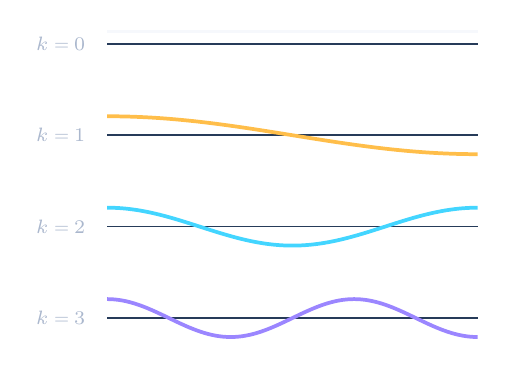
\begin{tikzpicture}[x=0.84cm,y=0.86cm]
        \foreach \y/\n in {
          4.55/0,
          3.20/1,
          1.85/2,
          0.50/3
        }{
          \draw[HydraLine,line width=0.55pt] (0.50,\y) -- (6.10,\y);
          \node[anchor=east,text=HydraMuted,
            font=\fontsize{7}{8.4}\selectfont]
            at (0.32,\y) {$k=\n$};
        }

        \draw[HydraWhite,line width=1.35pt] (0.50,4.73) -- (6.10,4.73);
        \draw[HydraGold,line width=1.35pt,domain=0.50:6.10,samples=100]
          plot (\x,{3.20+0.28*cos(180*(\x-0.50)/5.60)});
        \draw[HydraCyan,line width=1.35pt,domain=0.50:6.10,samples=100]
          plot (\x,{1.85+0.28*cos(360*(\x-0.50)/5.60)});
        \draw[HydraViolet,line width=1.35pt,domain=0.50:6.10,samples=100]
          plot (\x,{0.50+0.28*cos(540*(\x-0.50)/5.60)});
      \end{tikzpicture}

      \vspace{-0.05cm}

      {\color{HydraMuted}\fontsize{7.4}{9}\selectfont
        Each spatial shape will evolve independently after linearization.
      \par}
    \end{column}

  \end{columns}

\end{frame}


\begin{frame}{Each mode is a two-dimensional stability problem}

  \vspace{-0.26cm}

  {\color{HydraMuted}\fontsize{7.4}{9}\selectfont
    Combining the linearized perturbation equation with the eigenfunction expansion
  \par}

  \vspace{-0.12cm}

  \begin{columns}[c,onlytextwidth]

    \begin{column}{0.57\textwidth}
      {\color{HydraWhite}\fontsize{7.5}{9.3}\selectfont
      \begin{align*}
        \partial_t
        \begin{pmatrix}
          \eta\\
          \xi
        \end{pmatrix}
        &=
        J(\bar u,\bar v)
        \begin{pmatrix}
          \eta\\
          \xi
        \end{pmatrix}
        +
        \begin{pmatrix}
          D_u&0\\
          0&D_v
        \end{pmatrix}
        \Delta
        \begin{pmatrix}
          \eta\\
          \xi
        \end{pmatrix}
      \end{align*}
      }
    \end{column}

    \begin{column}{0.04\textwidth}
      \centering
      {\color{HydraGold}\bfseries\fontsize{15}{15}\selectfont
        $+$
      }
    \end{column}

    \begin{column}{0.35\textwidth}
      {\color{HydraWhite}\fontsize{7.9}{9.8}\selectfont
      \begin{align*}
        \begin{pmatrix}
          \eta(x,t)\\
          \xi(x,t)
        \end{pmatrix}
        &=
        \sum_{k=0}^{\infty}
        \begin{pmatrix}
          a_k(t)\\
          b_k(t)
        \end{pmatrix}
        \phi_k(x)
      \end{align*}
      }
    \end{column}

  \end{columns}

  \vspace{0.14cm}

  \begin{columns}[c,onlytextwidth]
    \begin{column}{0.57\textwidth}
      \mbox{}
    \end{column}

    \begin{column}{0.04\textwidth}
      \centering
      {\color{HydraCyan}\fontsize{15}{15}\selectfont
        $\Downarrow$
      }
    \end{column}

    \begin{column}{0.35\textwidth}
      \mbox{}
    \end{column}
  \end{columns}

  \vspace{0.14cm}

  {\color{HydraWhite}\fontsize{7.7}{9.6}\selectfont
  \begin{align*}
    \sum_{k=0}^{\infty}
    \frac{d}{dt}
    \binom{a_k}{b_k}
    \phi_k
    &=
    J(\bar u,\bar v)
    \sum_{k=0}^{\infty}
    \binom{a_k}{b_k}
    \phi_k
    +
    \begin{pmatrix}
      D_u&0\\
      0&D_v
    \end{pmatrix}
    \sum_{k=0}^{\infty}
    \binom{a_k}{b_k}
    \Delta\phi_k
  \end{align*}
  }

  \vspace{-0.30cm}

  {\color{HydraMuted}\fontsize{7.4}{9}\selectfont
    Since $\Delta\phi_k=-\mu_k\phi_k$ and
    $\{\phi_k\}_{k=0}^{\infty}$ is an orthonormal basis,
    the coefficients of every $\phi_k$ must agree
  \par}

  \vspace{-0.20cm}

  {\color{HydraWhite}\bfseries\fontsize{9.4}{11.8}\selectfont
  \begin{align*}
    \boxed{
      \frac{d}{dt}
      \binom{a_k}{b_k}
      =
      \left(
        J(\bar u,\bar v)-\mu_k
        \begin{pmatrix}
          D_u&0\\
          0&D_v
        \end{pmatrix}
      \right)
      \binom{a_k}{b_k}
    }
  \end{align*}
  }

\end{frame}


\begin{frame}{Define the stability matrix of each mode}

  \vspace{-0.46cm}

  {\color{HydraWhite}\fontsize{9.2}{11.6}\selectfont
  \begin{align*}
    \frac{d}{dt}
    \binom{a_k}{b_k}
    =
    \left(
      J(\bar u,\bar v)-\mu_k
      \begin{pmatrix}
        D_u&0\\
        0&D_v
      \end{pmatrix}
    \right)
    \binom{a_k}{b_k}
  \end{align*}
  }

  \vspace{-0.30cm}

  {\color{HydraMuted}\fontsize{7.6}{9.2}\selectfont
    Define the stability matrix associated with the $k$th spatial mode
  \par}

  \vspace{-0.24cm}

  {\color{HydraWhite}\fontsize{8.7}{10.9}\selectfont
  \begin{align*}
    \boxed{
      \begin{aligned}
        M_k
        =
        J(\bar u,\bar v)-\mu_k
        \begin{pmatrix}
          D_u&0\\
          0&D_v
        \end{pmatrix}&=
        \begin{pmatrix}
          f_u(\bar u,\bar v)-D_u\mu_k
          &f_v(\bar u,\bar v)
          \\
          g_u(\bar u,\bar v)
          &g_v(\bar u,\bar v)-D_v\mu_k
        \end{pmatrix}
      \end{aligned}
    }
  \end{align*}
  }

  \vspace{-0.34cm}

  {\color{HydraWhite}\bfseries\fontsize{11.2}{14}\selectfont
  \begin{align*}
    \boxed{
      \frac{d}{dt}
      \binom{a_k}{b_k}
      =
      M_k
      \binom{a_k}{b_k}
    }
  \end{align*}
  }

  \vspace{-0.28cm}

  \HydraTakeaway{
    Every spatial wavelength has its own $2\times2$ stability matrix
  }

\end{frame}


\begin{frame}{The homogeneous mode remains locally stable}

  \vspace{-0.08cm}

  \begin{columns}[c,onlytextwidth]

    \begin{column}{0.47\textwidth}
      {\color{HydraGold}\bfseries\fontsize{8}{9.5}\selectfont
        HOMOGENEOUS MODE\par}

      \vspace{-0.12cm}

      {\color{HydraWhite}\fontsize{12}{15.2}\selectfont
      \[
        \phi_0(x)=\text{constant}
        \qquad
        \mu_0=0
      \]
      }

      \vspace{-0.20cm}

      {\color{HydraWhite}\bfseries\fontsize{13.2}{16.2}\selectfont
      \[
        \boxed{M_0=J(\bar u,\bar v)}
      \]
      }

      \vspace{-0.14cm}

      % REPLACEABLE VISUAL
      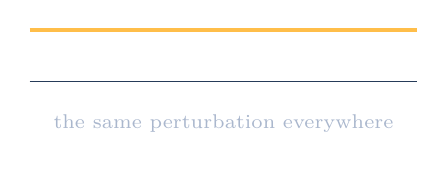
\begin{tikzpicture}[x=0.82cm,y=0.82cm]
        \draw[HydraLine,line width=0.6pt] (0.35,1.35) -- (6.35,1.35);
        \draw[HydraGold,line width=1.5pt] (0.35,2.15) -- (6.35,2.15);
        \node[anchor=north,text=HydraMuted,
          font=\fontsize{7.2}{8.7}\selectfont]
          at (3.35,0.98) {the same perturbation everywhere};
      \end{tikzpicture}

      \vspace{-0.10cm}

      \HydraPoint[HydraCyan]
        {Stable by assumption}
        {The local reaction analysis already guarantees decay of this mode.}
    \end{column}

    \begin{column}{0.04\textwidth}
      \centering
      {\color{HydraLine}\rule{0.7pt}{5.1cm}}
    \end{column}

    \begin{column}{0.45\textwidth}
      {\color{HydraCyan}\bfseries\fontsize{8}{9.5}\selectfont
        NONCONSTANT MODES\par}

      \vspace{-0.12cm}

      {\color{HydraWhite}\fontsize{12}{15.2}\selectfont
      \[
        \mu_k>0
        \qquad
        k\geq1
      \]
      }

      \vspace{-0.20cm}

      {\color{HydraWhite}\fontsize{10.2}{13}\selectfont
      \[
        M_k
        =
        J(\bar u,\bar v)-\mu_k
        \begin{pmatrix}
          D_u&0\\
          0&D_v
        \end{pmatrix}
      \]
      }

      \vspace{-0.16cm}

      % REPLACEABLE VISUAL
      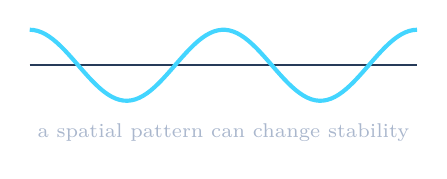
\begin{tikzpicture}[x=0.82cm,y=0.82cm]
        \draw[HydraLine,line width=0.6pt] (0.35,1.35) -- (6.35,1.35);
        \draw[HydraCyan,line width=1.5pt,domain=0.35:6.35,samples=100]
          plot (\x,{1.35+0.55*cos(360*2*(\x-0.35)/6.00)});
        \node[anchor=north,text=HydraMuted,
          font=\fontsize{7.2}{8.7}\selectfont]
          at (3.35,0.60) {a spatial pattern can change stability};
      \end{tikzpicture}

      \vspace{-0.10cm}

      \HydraPoint[HydraGold]
        {The Turing question}
        {Can any $M_k$ acquire an eigenvalue with positive real part?}
    \end{column}

  \end{columns}

\end{frame}


\begin{frame}{Diffusion makes the trace more negative}

  \vspace{-0.08cm}

  \begin{columns}[c,onlytextwidth]

    \begin{column}{0.57\textwidth}
      {\color{HydraWhite}\fontsize{10.2}{13}\selectfont
      \begin{align*}
        M_k
        =
        \begin{pmatrix}
          f_u(\bar u,\bar v)-D_u\mu_k&f_v(\bar u,\bar v)\\
          g_u(\bar u,\bar v)&g_v(\bar u,\bar v)-D_v\mu_k
        \end{pmatrix}
      \end{align*}
      }

      \vspace{-0.20cm}

      {\color{HydraWhite}\bfseries\fontsize{12.2}{15.2}\selectfont
      \begin{align*}
        \boxed{
          \operatorname{tr}(M_k)
          =
          \operatorname{tr}J(\bar u,\bar v)
          -
          (D_u+D_v)\mu_k
        }
      \end{align*}
      }

      \vspace{-0.16cm}

      \HydraPoint[HydraCyan]
        {The trace starts negative}
        {$\mu_0=0$ and $\operatorname{tr}(M_0)=\operatorname{tr}J(\bar u,\bar v)<0$ because the homogeneous equilibrium is locally stable.}

      \vspace{0.12cm}

      \HydraPoint[HydraGold]
        {Diffusion decreases it further}
        {For every $k\geq1$, the term $-(D_u+D_v)\mu_k$ is strictly negative.}

      \vspace{-0.08cm}

      {\color{HydraMuted}\fontsize{7.8}{9.5}\selectfont
        Therefore a Turing instability cannot occur through the trace becoming positive.
      \par}
    \end{column}

    \begin{column}{0.39\textwidth}
      \centering

      % REPLACEABLE VISUAL
      % Replace the tikzpicture with:
      % \includegraphics[width=\linewidth,height=4.80cm,keepaspectratio]{figures/turing/...}
      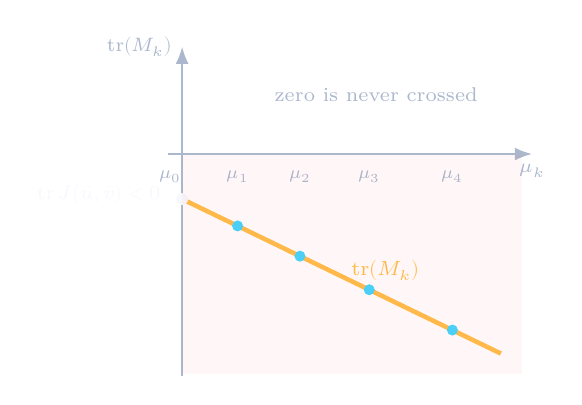
\begin{tikzpicture}[x=0.88cm,y=0.88cm]
        \draw[-{Latex[length=2.2mm]},HydraMuted,line width=0.75pt]
          (0.45,3.60) -- (5.70,3.60)
          node[below,text=HydraMuted,font=\fontsize{7}{8.2}\selectfont] {$\mu_k$};
        \draw[-{Latex[length=2.2mm]},HydraMuted,line width=0.75pt]
          (0.65,0.40) -- (0.65,5.15)
          node[left,text=HydraMuted,font=\fontsize{7}{8.2}\selectfont] {$\operatorname{tr}(M_k)$};

        \draw[HydraGold,line width=1.65pt]
          (0.65,2.95) -- (5.25,0.72);

        \fill[HydraWhite] (0.65,2.95) circle[radius=0.075cm];
        \foreach \x/\lab in {1.45/1,2.35/2,3.35/3,4.55/4}{
          \pgfmathsetmacro{\yy}{2.95-0.4848*(\x-0.65)}
          \fill[HydraCyan] (\x,\yy) circle[radius=0.070cm];
          \node[anchor=north,text=HydraMuted,
            font=\fontsize{6.4}{7.7}\selectfont]
            at (\x,3.50) {$\mu_{\lab}$};
        }
        \node[anchor=north,text=HydraMuted,
          font=\fontsize{6.4}{7.7}\selectfont]
          at (0.48,3.50) {$\mu_0$};

        \node[anchor=east,text=HydraWhite,
          font=\fontsize{7.2}{8.7}\selectfont]
          at (0.48,3.02) {$\operatorname{tr}J(\bar u,\bar v)<0$};

        \node[anchor=west,text=HydraGold,
          font=\bfseries\fontsize{7.4}{8.9}\selectfont]
          at (2.95,1.92) {$\operatorname{tr}(M_k)$};

        \fill[HydraRed,opacity=0.05] (0.65,0.42) rectangle (5.55,3.58);
        \node[text=HydraMuted,font=\fontsize{7.2}{8.7}\selectfont]
          at (3.45,4.45) {zero is never crossed};
      \end{tikzpicture}
    \end{column}

  \end{columns}

\end{frame}


\begin{frame}{The determinant contains the instability mechanism}

  \vspace{-0.08cm}

  {\color{HydraMuted}\fontsize{7.7}{9.4}\selectfont
    Compute the determinant of the mode matrix
  \par}

  \vspace{-0.16cm}

  {\color{HydraWhite}\fontsize{10}{12.7}\selectfont
  \begin{align*}
    \det(M_k)
    &=
    \det
    \begin{pmatrix}
      f_u(\bar u,\bar v)-D_u\mu_k&f_v(\bar u,\bar v)\\
      g_u(\bar u,\bar v)&g_v(\bar u,\bar v)-D_v\mu_k
    \end{pmatrix}
    \\
    &=
    \left(f_u(\bar u,\bar v)-D_u\mu_k\right)
    \left(g_v(\bar u,\bar v)-D_v\mu_k\right)
    -f_v(\bar u,\bar v)g_u(\bar u,\bar v)
    \\
    &=
    \det J(\bar u,\bar v)
    -
    \left(D_vf_u(\bar u,\bar v)+D_ug_v(\bar u,\bar v)\right)\mu_k
    +
    D_uD_v\mu_k^2
  \end{align*}
  }

  \vspace{-0.32cm}

  {\color{HydraWhite}\bfseries\fontsize{10.4}{13.2}\selectfont
  \begin{align*}
    {\color{HydraGold}
      \boxed{
        \det(M_k)
        =
        \det J(\bar u,\bar v)-A\mu_k+D_uD_v\mu_k^2
      }
    }
    \qquad
    A=D_vf_u(\bar u,\bar v)+D_ug_v(\bar u,\bar v)
  \end{align*}
  }

  \vspace{-0.14cm}

  \begin{columns}[T,onlytextwidth]
    \begin{column}{0.31\textwidth}
      \HydraPoint[HydraCyan]
        {Positive at $\mu_0=0$}
        {$\det(M_0)=\det J(\bar u,\bar v)>0$ follows from local stability.}
    \end{column}

    \begin{column}{0.31\textwidth}
      \HydraPoint[HydraGold]
        {The linear term can decrease it}
        {Unequal diffusion weights $f_u$ and $g_v$ differently inside $A$.}
    \end{column}

    \begin{column}{0.31\textwidth}
      \HydraPoint[HydraGold]
        {Very short waves are stable}
        {$D_uD_v\mu_k^2$ dominates for sufficiently large $k$.}
    \end{column}
  \end{columns}

\end{frame}


\begin{frame}{Turing instability condition}

  \vspace{-0.24cm}

  \begin{columns}[c,onlytextwidth]

    \begin{column}{0.57\textwidth}

      \vspace{-0.30cm}

      {\color{HydraWhite}\bfseries\fontsize{10.4}{13.2}\selectfont
      \begin{align*}
        {\color{HydraGold}
          \boxed{
            \det(M_k)
            =
            \det J(\bar u,\bar v)-A\mu_k+D_uD_v\mu_k^2
          }
        }
      \end{align*}
      }

      \vspace{-0.44cm}

      \HydraPoint[HydraCyan]
        {$\det(M_k)>0$}
        {The $k$th spatial mode is stable.}

      \vspace{-0.0cm}

      \HydraPoint[HydraGold]
        {$\det(M_k)<0$}
        {The $k$th spatial mode is unstable.}

      \vspace{-0.3cm}

{\color{HydraWhite}\fontsize{9.5}{12}\selectfont
      \begin{align*}
        \det(M_k)<0
        \quad\Longleftrightarrow\quad
        \mu_-<\mu_k<\mu_+
      \end{align*}
      }

      \vspace{-0.3cm}
      {\color{HydraMuted}\fontsize{7.4}{9.1}\selectfont
        A negative interval exists when
      \par}

      \vspace{-0.62cm}

      {\color{HydraWhite}\fontsize{9.5}{12}\selectfont
      \begin{align*}
        A>0
        \qquad
        A^2>4D_uD_v\det J(\bar u,\bar v)
      \end{align*}
      }

      \vspace{-0.80cm}

      {\color{HydraWhite}\fontsize{8.8}{11.1}\selectfont
      \begin{align*}
        \mu_\pm
        =
        \frac{
          A\pm\sqrt{A^2-4D_uD_v\det J(\bar u,\bar v)}
        }{
          2D_uD_v
        }
      \end{align*}
      }
    \end{column}

    \begin{column}{0.39\textwidth}
      \centering

      % REPLACEABLE VISUAL
      % Replace the tikzpicture with:
      % \includegraphics[width=\linewidth,height=4.95cm,keepaspectratio]{figures/turing/...}
      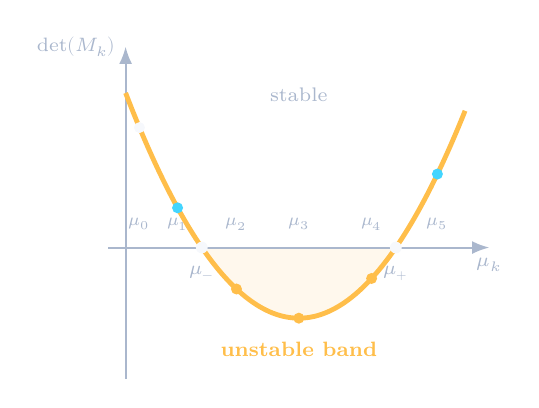
\begin{tikzpicture}[x=0.88cm,y=0.88cm]
        \fill[HydraGold,opacity=0.10]
          plot[domain=1.75:4.55,samples=100]
            (\x,{2.35+0.52*(\x-1.75)*(\x-4.55)})
          -- (4.55,2.35) -- (1.75,2.35) -- cycle;

        \draw[-{Latex[length=2.2mm]},HydraMuted,line width=0.75pt]
          (0.40,2.35) -- (5.90,2.35)
          node[below,text=HydraMuted,font=\fontsize{7}{8.2}\selectfont] {$\mu_k$};
        \draw[-{Latex[length=2.2mm]},HydraMuted,line width=0.75pt]
          (0.65,0.45) -- (0.65,5.25)
          node[left,text=HydraMuted,font=\fontsize{7}{8.2}\selectfont] {$\det(M_k)$};

        \draw[HydraGold,line width=1.75pt,domain=0.65:5.55,samples=100]
          plot (\x,{2.35+0.52*(\x-1.75)*(\x-4.55)});

        \foreach \x/\lab/\col in {0.85/0/HydraWhite,1.40/1/HydraCyan,2.25/2/HydraGold,3.15/3/HydraGold,4.20/4/HydraGold,5.15/5/HydraCyan}{
          \pgfmathsetmacro{\yy}{2.35+0.52*(\x-1.75)*(\x-4.55)}
          \fill[\col] (\x,\yy) circle[radius=0.070cm];
          \node[anchor=south,text=HydraMuted,
            font=\fontsize{6.2}{7.5}\selectfont]
            at (\x,2.46) {$\mu_{\lab}$};
        }

        \fill[HydraWhite] (1.75,2.35) circle[radius=0.075cm];
        \fill[HydraWhite] (4.55,2.35) circle[radius=0.075cm];

        \node[anchor=north,text=HydraMuted,
          font=\fontsize{6.9}{8.3}\selectfont]
          at (1.75,2.22) {$\mu_-$};
        \node[anchor=north,text=HydraMuted,
          font=\fontsize{6.9}{8.3}\selectfont]
          at (4.55,2.22) {$\mu_+$};

        \node[text=HydraGold,font=\bfseries\fontsize{7.5}{9}\selectfont]
          at (3.15,0.88) {unstable band};
        \node[text=HydraMuted,font=\fontsize{7.1}{8.6}\selectfont]
          at (3.15,4.55) {stable};
      \end{tikzpicture}
    \end{column}

  \end{columns}

\end{frame}


\begin{frame}{Turing instability theorem}

  \vspace{-0.28cm}

  {\color{HydraWhite}\bfseries\fontsize{9.8}{12.5}\selectfont
  \begin{align*}
    \boxed{
      \begin{aligned}
        \partial_tu&=D_u\Delta u+f(u,v)
        \\
        \partial_tv&=D_v\Delta v+g(u,v)
      \end{aligned}
    }
  \end{align*}
  }

  \vspace{+0.34cm}

  {\color{HydraGold}\bfseries\fontsize{7.8}{9.4}\selectfont
    THEOREM\par}

  \vspace{0.14cm}

  {\color{HydraWhite}\fontsize{9.2}{12}\selectfont
    If the system is stable in the absence of diffusion, and $u$ satisfies the autocatalysis condition, i.e.
    $f_u(\bar u,\bar v)>0$, diffusion $D_u$ is sufficiently small and diffusion $D_v$ is
    sufficiently large, then diffusion destabilizes the homogeneous steady
    state $(\bar u,\bar v)$.
  \par}

\end{frame}


\HydraSubsection[
  \mbox{The unstable band must intersect}
  \mbox{the discrete spatial spectrum}
  \mbox{allowed by the tissue geometry}
]{Mode selection}


\begin{frame}{Only eigenvalues inside the unstable band can grow}

  \vspace{-0.08cm}

  \begin{columns}[c,onlytextwidth]
    \begin{column}{0.72\textwidth}
      \centering

      % REPLACEABLE VISUAL
      % Replace the tikzpicture with the user's unstable-eigenmodes figure:
      % \includegraphics[width=\linewidth,height=5.20cm,keepaspectratio]{figures/turing/...}
      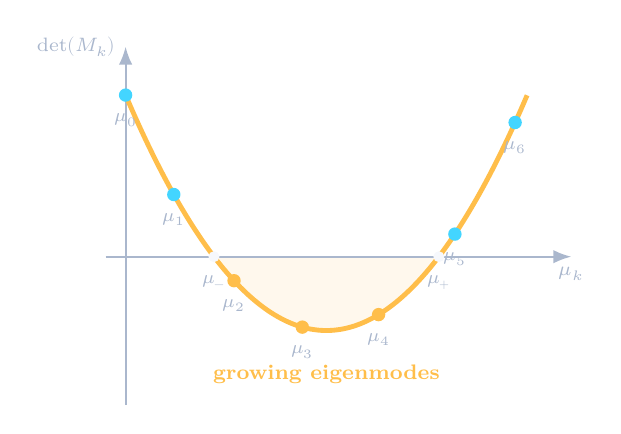
\begin{tikzpicture}[x=1.02cm,y=0.92cm]
        \fill[HydraGold,opacity=0.10]
          plot[domain=1.75:4.55,samples=100]
            (\x,{2.35+0.52*(\x-1.75)*(\x-4.55)})
          -- (4.55,2.35) -- (1.75,2.35) -- cycle;

        \draw[-{Latex[length=2.3mm]},HydraMuted,line width=0.75pt]
          (0.40,2.35) -- (6.20,2.35)
          node[below,text=HydraMuted,font=\fontsize{7}{8.2}\selectfont] {$\mu_k$};
        \draw[-{Latex[length=2.3mm]},HydraMuted,line width=0.75pt]
          (0.65,0.30) -- (0.65,5.25)
          node[left,text=HydraMuted,font=\fontsize{7}{8.2}\selectfont] {$\det(M_k)$};

        \draw[HydraGold,line width=1.75pt,domain=0.65:5.65,samples=120]
          plot (\x,{2.35+0.52*(\x-1.75)*(\x-4.55)});

        \foreach \x/\lab/\col in {0.65/0/HydraCyan,1.25/1/HydraCyan,2.00/2/HydraGold,2.85/3/HydraGold,3.80/4/HydraGold,4.75/5/HydraCyan,5.50/6/HydraCyan}{
          \pgfmathsetmacro{\yy}{2.35+0.52*(\x-1.75)*(\x-4.55)}
          \fill[\col] (\x,\yy) circle[radius=0.085cm];
          \node[anchor=north,text=HydraMuted,
            font=\fontsize{6.6}{8}\selectfont]
            at (\x,{\yy-0.12}) {$\mu_{\lab}$};
        }

        \fill[HydraWhite] (1.75,2.35) circle[radius=0.070cm];
        \fill[HydraWhite] (4.55,2.35) circle[radius=0.070cm];
        \node[anchor=north,text=HydraMuted,
          font=\fontsize{6.6}{8}\selectfont]
          at (1.75,2.22) {$\mu_-$};
        \node[anchor=north,text=HydraMuted,
          font=\fontsize{6.6}{8}\selectfont]
          at (4.55,2.22) {$\mu_+$};

        \node[text=HydraGold,font=\bfseries\fontsize{7.6}{9.1}\selectfont]
          at (3.15,0.72) {growing eigenmodes};
      \end{tikzpicture}
    \end{column}

    \begin{column}{0.24\textwidth}
      \HydraPoint[HydraGold]
        {Only selected modes grow}
        {The unstable band is continuous, but the tissue supplies only discrete eigenvalues.}
    \end{column}
  \end{columns}

  \vspace{0.46cm}

  \begin{columns}[c,onlytextwidth]
    \begin{column}{0.19\textwidth}
      \centering
      {\color{HydraWhite}\bfseries\fontsize{10.2}{12.9}\selectfont
        $\det(M_k)<0$
      \par}
    \end{column}

    \begin{column}{0.07\textwidth}
      \centering
      {\color{HydraCyan}\fontsize{17}{17}\selectfont
        $\Rightarrow$
      \par}
    \end{column}

    \begin{column}{0.29\textwidth}
      \centering
      {\color{HydraWhite}\fontsize{8.2}{10.4}\selectfont
        Exists a positive eigenvalue $\lambda_{k,+}$ 
      \par}
    \end{column}

    \begin{column}{0.07\textwidth}
      \centering
      {\color{HydraCyan}\fontsize{17}{17}\selectfont
        $\Rightarrow$
      \par}
    \end{column}

    \begin{column}{0.30\textwidth}
      \centering
      {\color{HydraWhite}\fontsize{8.2}{10.4}\selectfont
        Spatial mode $k$ grows at rate $e^{\lambda_{k,+}t}$
      \par}
    \end{column}
  \end{columns}

\end{frame}


\begin{frame}{Diffusion changes which modes are unstable}

  \vspace{-0.08cm}

  \begin{columns}[c,onlytextwidth]

    \begin{column}{0.67\textwidth}
      \centering

      % REPLACEABLE VISUAL
      % Replace the tikzpicture with:
      % \includegraphics[width=\linewidth,height=5.25cm,keepaspectratio]{figures/turing/...}
      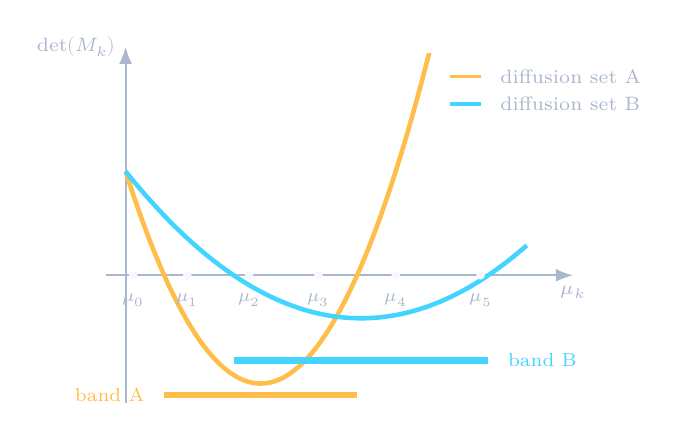
\begin{tikzpicture}[x=0.98cm,y=0.88cm]
        \draw[-{Latex[length=2.2mm]},HydraMuted,line width=0.75pt]
          (0.40,2.15) -- (6.45,2.15)
          node[below,text=HydraMuted,font=\fontsize{7}{8.2}\selectfont] {$\mu_k$};
        \draw[-{Latex[length=2.2mm]},HydraMuted,line width=0.75pt]
          (0.65,0.30) -- (0.65,5.45)
          node[left,text=HydraMuted,font=\fontsize{7}{8.2}\selectfont] {$\det(M_k)$};

        \begin{scope}
          \clip (0.40,0.30) rectangle (6.20,5.35);
          \draw[HydraGold,line width=1.65pt,domain=0.65:5.85,samples=120]
            plot (\x,{2.15+1.00*(\x-1.15)*(\x-3.65)});
          \draw[HydraCyan,line width=1.65pt,domain=0.65:5.85,samples=120]
            plot (\x,{2.15+0.228*(\x-2.05)*(\x-5.35)});
        \end{scope}

        \foreach \x/\lab in {
          0.75/0,
          1.45/1,
          2.25/2,
          3.15/3,
          4.15/4,
          5.25/5
        }{
          \fill[HydraWhite] (\x,2.15) circle[radius=0.055cm];
          \node[anchor=north,text=HydraMuted,
            font=\fontsize{6.5}{7.8}\selectfont]
            at (\x,2.02) {$\mu_{\lab}$};
        }

        \draw[HydraGold,line width=1.25pt] (4.85,5.02) -- (5.25,5.02);
        \node[anchor=west,text=HydraMuted,
          font=\fontsize{7}{8.4}\selectfont]
          at (5.38,5.02) {diffusion set A};
        \draw[HydraCyan,line width=1.25pt] (4.85,4.62) -- (5.25,4.62);
        \node[anchor=west,text=HydraMuted,
          font=\fontsize{7}{8.4}\selectfont]
          at (5.38,4.62) {diffusion set B};

        \draw[HydraGold,line width=2.2pt] (1.15,0.42) -- (3.65,0.42);
        \draw[HydraCyan,line width=2.2pt] (2.05,0.92) -- (5.35,0.92);
        \node[anchor=east,text=HydraGold,
          font=\fontsize{6.8}{8.2}\selectfont]
          at (1.02,0.42) {band A};
        \node[anchor=west,text=HydraCyan,
          font=\fontsize{6.8}{8.2}\selectfont]
          at (5.48,0.92) {band B};
      \end{tikzpicture}
    \end{column}

    \begin{column}{0.29\textwidth}
      \HydraPoint[HydraGold]
        {The band moves}
        {Changing $D_u$ and $D_v$ changes its location and width.}

      \vspace{0.10cm}

      \HydraPoint[HydraCyan]
        {The selected modes change}
        {A different set of the fixed eigenvalues $\mu_k$ can become unstable.}

      \vspace{0.04cm}

      {\color{HydraMuted}\fontsize{7.5}{9.1}\selectfont
        Diffusion therefore controls the preferred spatial scale.
      \par}
    \end{column}

  \end{columns}

  \vspace{-0.24cm}

  \begin{columns}[c,onlytextwidth]
    \begin{column}{0.67\textwidth}
      \centering
      {\color{HydraWhite}\fontsize{9.4}{12}\selectfont
      \begin{align*}
        \det(M_k)
        =
        \det J(\bar u,\bar v)-A\mu_k+D_uD_v\mu_k^2
      \end{align*}
      }
    \end{column}

    \begin{column}{0.29\textwidth}
    \end{column}
  \end{columns}

\end{frame}


\begin{frame}{Diffusion and domain size}

  \vspace{-0.08cm}

  \begin{columns}[c,onlytextwidth]

    \begin{column}{0.54\textwidth}
      {\color{HydraMuted}\fontsize{7.4}{9.1}\selectfont
        Let $\widetilde\Omega$ be a fixed reference domain and scale it by $L>0$
      \par}

      \vspace{-0.34cm}

      {\color{HydraWhite}\fontsize{9.8}{12.5}\selectfont
      \begin{align*}
        \Omega_L=L\widetilde\Omega
        \qquad
        x=L\widetilde x
      \end{align*}
      }

      \vspace{-0.46cm}

      {\color{HydraMuted}\fontsize{7.4}{9.1}\selectfont
        Under the change of variables $x=L\widetilde x$, the system is
        equivalently written on the reference domain as
      \par}

      \vspace{-0.34cm}

      {\color{HydraWhite}\fontsize{8.4}{10.7}\selectfont
      \begin{align*}
        \partial_t\widetilde u
        &=
        \frac{D_u}{L^2}\Delta_{\widetilde x}\widetilde u
        +f(\widetilde u,\widetilde v)
        \\
        \partial_t\widetilde v
        &=
        \frac{D_v}{L^2}\Delta_{\widetilde x}\widetilde v
        +g(\widetilde u,\widetilde v)
      \end{align*}
      }

      \vspace{-0.50cm}

      {\color{HydraGold}\bfseries\fontsize{8.1}{10.3}\selectfont
      \begin{align*}
        L\widetilde\Omega\ \text{with }(D_u,D_v)
        \quad\Leftrightarrow\quad
        \widetilde\Omega\ \text{with }
        \left(\frac{D_u}{L^2},\frac{D_v}{L^2}\right)
      \end{align*}
      }
    \end{column}

    \begin{column}{0.42\textwidth}
      \centering

      % REPLACEABLE VISUAL
      % Replace the tikzpicture with:
      % \includegraphics[width=\linewidth,height=4.95cm,keepaspectratio]{figures/turing/...}
      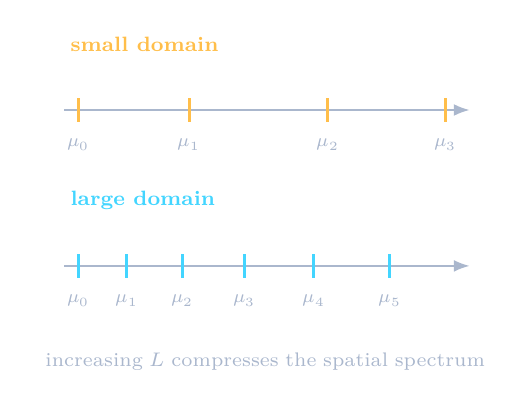
\begin{tikzpicture}[x=0.88cm,y=0.88cm]
        \node[anchor=west,text=HydraGold,
          font=\bfseries\fontsize{7.5}{9}\selectfont]
          at (0.30,5.10) {small domain};
        \draw[-{Latex[length=2mm]},HydraMuted,line width=0.70pt]
          (0.35,4.15) -- (6.20,4.15);
        \foreach \x/\lab in {0.55/0,2.15/1,4.15/2,5.85/3}{
          \draw[HydraGold,line width=1.1pt] (\x,3.98) -- (\x,4.32);
          \node[anchor=north,text=HydraMuted,
            font=\fontsize{6.5}{7.8}\selectfont]
            at (\x,3.88) {$\mu_{\lab}$};
        }

        \node[anchor=west,text=HydraCyan,
          font=\bfseries\fontsize{7.5}{9}\selectfont]
          at (0.30,2.85) {large domain};
        \draw[-{Latex[length=2mm]},HydraMuted,line width=0.70pt]
          (0.35,1.90) -- (6.20,1.90);
        \foreach \x/\lab in {
          0.55/0,
          1.25/1,
          2.05/2,
          2.95/3,
          3.95/4,
          5.05/5
        }{
          \draw[HydraCyan,line width=1.1pt] (\x,1.73) -- (\x,2.07);
          \node[anchor=north,text=HydraMuted,
            font=\fontsize{6.5}{7.8}\selectfont]
            at (\x,1.63) {$\mu_{\lab}$};
        }

        \node[anchor=north,text=HydraMuted,text width=5.8cm,align=center,
          font=\fontsize{7.1}{8.6}\selectfont]
          at (3.25,0.78)
          {increasing $L$ compresses the spatial spectrum};
      \end{tikzpicture}

      \vspace{-0.06cm}

      \HydraPoint[HydraGold]
        {Important distinction}
        {Changing the ratio $D_v/D_u$ is not equivalent to changing the domain size.}
    \end{column}

  \end{columns}

\end{frame}


\begin{frame}{A larger domain can support more peaks}

  \vspace{-0.14cm}

  \begin{columns}[T,onlytextwidth]

    \begin{column}{0.47\textwidth}
      \centering

      {\color{HydraGold}\bfseries\fontsize{8}{9.5}\selectfont
        SMALL DOMAIN\par}

      \vspace{0.08cm}

      % REPLACEABLE VISUAL
      % Replace the tikzpicture with:
      % \includegraphics[width=\linewidth,height=3.45cm,keepaspectratio]{figures/turing/...}
      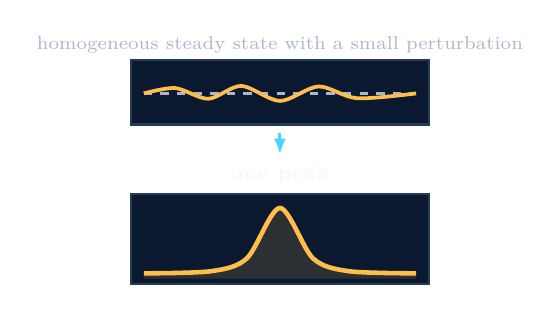
\begin{tikzpicture}[x=0.70cm,y=0.68cm]
        \node[text=HydraMuted,font=\fontsize{6.7}{8}\selectfont]
          at (2.95,4.66) {homogeneous steady state with a small perturbation};

        \fill[HydraPanel] (0.25,3.18) rectangle (5.65,4.38);
        \draw[HydraLine,line width=0.8pt] (0.25,3.18) rectangle (5.65,4.38);
        \draw[HydraMuted,line width=0.8pt,dashed] (0.48,3.76) -- (5.42,3.76);
        \draw[HydraGold,line width=1.35pt]
          plot[smooth] coordinates {
            (0.48,3.76) (1.05,3.86) (1.65,3.66) (2.25,3.90)
            (2.95,3.62) (3.65,3.89) (4.35,3.67) (5.42,3.76)
          };

        \draw[-{Latex[length=2mm]},HydraCyan,line width=1.1pt]
          (2.95,3.02) -- (2.95,2.62);

        \node[text=HydraWhite,font=\bfseries\fontsize{7.1}{8.5}\selectfont]
          at (2.95,2.25) {one peak};

        \fill[HydraPanel] (0.25,0.20) rectangle (5.65,1.88);
        \draw[HydraLine,line width=0.8pt] (0.25,0.20) rectangle (5.65,1.88);
        \fill[HydraGold,opacity=0.14]
          plot[smooth] coordinates {
            (0.48,0.40) (1.70,0.44) (2.35,0.68) (2.95,1.62)
            (3.55,0.68) (4.20,0.44) (5.42,0.40)
          } -- (5.42,0.30) -- (0.48,0.30) -- cycle;
        \draw[HydraGold,line width=1.65pt]
          plot[smooth] coordinates {
            (0.48,0.40) (1.70,0.44) (2.35,0.68) (2.95,1.62)
            (3.55,0.68) (4.20,0.44) (5.42,0.40)
          };
      \end{tikzpicture}
    \end{column}

    \begin{column}{0.47\textwidth}
      \centering

      {\color{HydraCyan}\bfseries\fontsize{8}{9.5}\selectfont
        LARGER DOMAIN\par}

      \vspace{0.08cm}

      % REPLACEABLE VISUAL
      % Replace the tikzpicture with:
      % \includegraphics[width=\linewidth,height=3.45cm,keepaspectratio]{figures/turing/...}
      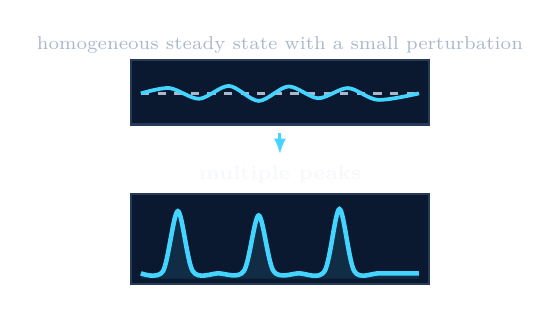
\begin{tikzpicture}[x=0.54cm,y=0.68cm]
        \node[text=HydraMuted,font=\fontsize{6.7}{8}\selectfont]
          at (3.75,4.66) {homogeneous steady state with a small perturbation};

        \fill[HydraPanel] (0.25,3.18) rectangle (7.25,4.38);
        \draw[HydraLine,line width=0.8pt] (0.25,3.18) rectangle (7.25,4.38);
        \draw[HydraMuted,line width=0.8pt,dashed] (0.48,3.76) -- (7.02,3.76);
        \draw[HydraCyan,line width=1.35pt]
          plot[smooth] coordinates {
            (0.48,3.76) (1.15,3.86) (1.85,3.66) (2.55,3.90)
            (3.25,3.62) (3.95,3.89) (4.65,3.67) (5.35,3.86)
            (6.05,3.64) (7.02,3.76)
          };

        \draw[-{Latex[length=2mm]},HydraCyan,line width=1.1pt]
          (3.75,3.02) -- (3.75,2.62);

        \node[text=HydraWhite,font=\bfseries\fontsize{7.1}{8.5}\selectfont]
          at (3.75,2.25) {multiple peaks};

        \fill[HydraPanel] (0.25,0.20) rectangle (7.25,1.88);
        \draw[HydraLine,line width=0.8pt] (0.25,0.20) rectangle (7.25,1.88);
        \fill[HydraCyan,opacity=0.11]
          plot[smooth] coordinates {
            (0.48,0.40)
            (1.00,0.44) (1.35,1.56) (1.70,0.44)
            (2.30,0.40)
            (2.90,0.44) (3.25,1.48) (3.60,0.44)
            (4.20,0.40)
            (4.80,0.44) (5.15,1.60) (5.50,0.44)
            (6.10,0.40) (7.02,0.40)
          } -- (7.02,0.30) -- (0.48,0.30) -- cycle;
        \draw[HydraCyan,line width=1.65pt]
          plot[smooth] coordinates {
            (0.48,0.40)
            (1.00,0.44) (1.35,1.56) (1.70,0.44)
            (2.30,0.40)
            (2.90,0.44) (3.25,1.48) (3.60,0.44)
            (4.20,0.40)
            (4.80,0.44) (5.15,1.60) (5.50,0.44)
            (6.10,0.40) (7.02,0.40)
          };
      \end{tikzpicture}
    \end{column}

  \end{columns}

  \vspace{1.08cm}

  \begin{columns}[T,onlytextwidth]
    \begin{column}{0.31\textwidth}
      \HydraPoint[HydraGold]
        {Linear level}
        {Turing analysis identifies which modes lie in the unstable band and can grow}
    \end{column}

    \begin{column}{0.31\textwidth}
      \HydraPoint[HydraCyan]
        {Pattern formation requires nonlinearity}
        {Nonlinear interactions select and saturate the emerging spatial pattern}
    \end{column}

    \begin{column}{0.31\textwidth}
      \HydraPoint[HydraGold]
        {Useful but incomplete prediction}
        {Unstable eigenmodes can be useful for predicting the pattern, but they do not provide a complete explanation}
    \end{column}
  \end{columns}

\end{frame}

\input{sections/GiererMeinhardt.tex}
\HydraSection[
  focus x=0.62,
  focus y=0.65,
  radius=0.14,
  zoom=1.85
]{Growth, wounds \& long-range dynamics}


% \HydraSubsection[
%   \mbox{Patterns are stable nonconstant}
%   \mbox{steady states of the full}
%   \mbox{nonlinear reaction--diffusion system}
% ]{What is a pattern?}


\begin{frame}{What do we mean by a pattern?}

  \vspace{-0.34cm}

  \begin{columns}[T,onlytextwidth]

    \begin{column}{0.48\textwidth}
      {\color{HydraMuted}\fontsize{7.5}{9.2}\selectfont
        Return to the Gierer--Meinhardt system
      \par}

      \vspace{-0.30cm}

      {\color{HydraWhite}\fontsize{9.0}{11.5}\selectfont
      \begin{align*}
        \partial_tu
        &=
        D_u\Delta u
        +
        \frac{au^2}{K+v}
        -
        \mu_u u
        \\
        \partial_tv
        &=
        D_v\Delta v
        +
        bu^2
        -
        \mu_v v
      \end{align*}
      }

      \vspace{-0.42cm}

      {\color{HydraMuted}\fontsize{7.3}{9}\selectfont
        with homogeneous Neumann boundary conditions on $\Omega$
      \par}
    \end{column}

    \begin{column}{0.48\textwidth}
      {\centering\color{HydraGold}\bfseries\fontsize{7.5}{9.2}\selectfont
        STEADY STATE\par}

      \vspace{-0.30cm}

      {\color{HydraWhite}\fontsize{8.2}{10.4}\selectfont
      \begin{align*}
        0
        &=
        D_u\Delta\bar u
        +
        \frac{a\bar u^2}{K+\bar v}
        -
        \mu_u\bar u
        \\
        0
        &=
        D_v\Delta\bar v
        +
        b\bar u^2
        -
        \mu_v\bar v
      \end{align*}
      }

      \vspace{-0.42cm}

      \HydraPoint[HydraCyan]
        {Spatial pattern}
        {A stable nonconstant steady state $(\bar u(x),\bar v(x))$}
    \end{column}

  \end{columns}

  \vspace{0.22cm}

  \HydraTakeaway{
    For nonlinear reaction--diffusion systems, a complete characterization of all steady states is generally not known
  }

\end{frame}


\HydraSubsection[
  \mbox{Growth and division change both}
  \mbox{the geometry and the initial data}
  \mbox{of the nonlinear problem}
]{Growth and \mbox{division}}


\begin{frame}{Growth makes the domain part of the dynamics}

  \vspace{-0.12cm}

  \begin{columns}[c,onlytextwidth]
    \begin{column}{0.46\textwidth}
      {\color{HydraGold}\bfseries\fontsize{7.6}{9.1}\selectfont
        TIME-DEPENDENT DOMAIN\par}

      \vspace{-0.16cm}

      {\color{HydraWhite}\bfseries\fontsize{12}{15.2}\selectfont
      \begin{align*}
        \Omega(t)&=[0,L(t)]
        \\
        L'(t)&>0
      \end{align*}
      }

      \vspace{-0.38cm}

      \HydraPoint[HydraCyan]
        {Changing geometry}
        {Growth changes physical distances and the spatial structures that fit inside the domain}

      \vspace{-0.08cm}

      \HydraPoint[HydraGold]
        {Nonlinear question}
        {Does the current pattern persist, reorganize, or generate additional peaks}
    \end{column}

    \begin{column}{0.50\textwidth}
      \centering

      % REPLACEABLE VISUAL
      % Replace the tikzpicture with:
      % \includegraphics[width=\linewidth,height=4.95cm,keepaspectratio]{figures/simulations/growing_domain.png}
      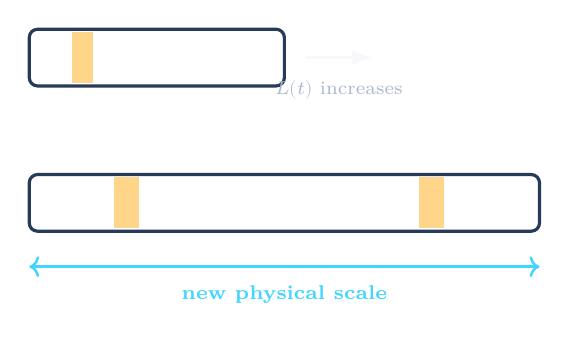
\begin{tikzpicture}[x=0.90cm,y=0.90cm]
        \draw[HydraLine,line width=1.15pt,rounded corners=3pt]
          (0.45,3.30) rectangle (4.05,4.10);
        \fill[HydraGold,opacity=0.65] (1.05,3.34) rectangle (1.35,4.06);

        \draw[-{Latex[length=2.6mm]},HydraWhite,line width=1.0pt]
          (4.35,3.70) -- (5.30,3.70);
        \node[text=HydraMuted,font=\fontsize{6.8}{8.2}\selectfont]
          at (4.82,3.25) {$L(t)$ increases};

        \draw[HydraLine,line width=1.15pt,rounded corners=3pt]
          (0.45,1.25) rectangle (7.65,2.05);
        \fill[HydraGold,opacity=0.65] (1.65,1.29) rectangle (2.00,2.01);
        \fill[HydraGold,opacity=0.65] (5.95,1.29) rectangle (6.30,2.01);

        \draw[<->,HydraCyan,line width=0.9pt]
          (0.45,0.75) -- (7.65,0.75);
        \node[text=HydraCyan,font=\bfseries\fontsize{7.2}{8.6}\selectfont]
          at (4.05,0.35) {new physical scale};
      \end{tikzpicture}
    \end{column}
  \end{columns}

  \vspace{-0.10cm}

  \HydraTakeaway{
    The concentrations evolve while the domain supporting them changes
  }
\end{frame}


% \begin{frame}{The growth experiment begins from a one-peak pattern}

%   \vspace{-0.12cm}

%   \begin{columns}[c,onlytextwidth]
%     \begin{column}{0.70\textwidth}
%       \centering

%       % REPLACEABLE VISUAL
%       % Replace the tikzpicture with:
%       % \includegraphics[width=\linewidth,height=5.25cm,keepaspectratio]{figures/simulations/short_domain_single_peak.png}
%       \begin{tikzpicture}[x=0.90cm,y=0.90cm]
%         \draw[-{Latex[length=2mm]},HydraMuted,line width=0.7pt]
%           (0.45,0.75) -- (8.75,0.75)
%           node[below,text=HydraMuted,font=\fontsize{7}{8.2}\selectfont] {$x$};
%         \draw[HydraGold,line width=1.70pt]
%           plot[smooth] coordinates {(0.55,0.80) (2.10,0.85) (3.25,1.08) (3.85,2.10) (4.20,4.85) (4.58,2.10) (5.15,1.08) (6.30,0.85) (8.60,0.80)};
%         \draw[HydraCyan,line width=1.45pt]
%           plot[smooth] coordinates {(0.55,1.05) (1.70,1.35) (2.80,1.85) (4.20,2.45) (5.65,1.85) (6.85,1.35) (8.60,1.05)};
%         \node[text=HydraGold,font=\bfseries\fontsize{7.2}{8.6}\selectfont]
%           at (5.15,4.55) {$\bar u_1(x)$};
%         \node[text=HydraCyan,font=\bfseries\fontsize{7.2}{8.6}\selectfont]
%           at (6.80,2.15) {$\bar v_1(x)$};
%       \end{tikzpicture}
%     \end{column}

%     \begin{column}{0.26\textwidth}
%       \HydraPoint[HydraGold]
%         {Reference pattern}
%         {For the chosen parameters the initial domain supports a stable one-peak steady state}

%       \vspace{-0.18cm}

%       \HydraPoint[HydraCyan]
%         {Initial condition}
%         {The growth simulation starts from $(\bar u_1(x),\bar v_1(x))$}
%     \end{column}
%   \end{columns}
% \end{frame}


\begin{frame}{Growth can transform one stable pattern into another}

  \vspace{-0.14cm}

  \centering

  % REPLACEABLE VISUAL
  % Replace the tikzpicture with:
  % \includegraphics[width=0.94\linewidth,height=5.30cm,keepaspectratio]{figures/simulations/growth_sequence.png}
  \begin{tikzpicture}[x=0.82cm,y=0.82cm]
    \foreach \shift/\width/\stage in {0/3.2/{$t_0$},4.0/4.7/{$t_1$},9.3/6.0/{$t_2$}}{
      \begin{scope}[shift={(\shift,0)}]
        \draw[HydraLine,line width=1.0pt,rounded corners=2pt]
          (0.20,0.65) rectangle (\width,1.25);
        \node[text=HydraMuted,font=\fontsize{7}{8.4}\selectfont]
          at ({0.5*\width},0.20) {\stage};
      \end{scope}
    }

    \fill[HydraGold,opacity=0.72] (1.38,0.69) rectangle (1.68,1.21);
    \fill[HydraGold,opacity=0.72] (4.75,0.69) rectangle (5.05,1.21);
    \fill[HydraGold,opacity=0.72] (7.65,0.69) rectangle (7.95,1.21);
    \fill[HydraGold,opacity=0.72] (10.20,0.69) rectangle (10.50,1.21);
    \fill[HydraGold,opacity=0.72] (13.65,0.69) rectangle (13.95,1.21);

    \draw[-{Latex[length=2.4mm]},HydraWhite,line width=1.0pt]
      (3.35,0.95) -- (3.85,0.95);
    \draw[-{Latex[length=2.4mm]},HydraWhite,line width=1.0pt]
      (8.85,0.95) -- (9.20,0.95);

    \node[text=HydraGold,font=\bfseries\fontsize{7.3}{8.7}\selectfont]
      at (7.65,3.95) {a new spatial structure can form as the domain grows};
    \node[text=HydraMuted,font=\fontsize{7}{8.5}\selectfont,align=center,text width=9.8cm]
      at (7.65,2.85) {the simulation follows the full nonlinear solution in the physical coordinate};
  \end{tikzpicture}

  \vspace{-0.12cm}

  \HydraTakeaway{
    Growth can reorganize an existing pattern instead of merely stretching it
  }
\end{frame}


\begin{frame}{Division creates two new initial-value problems}

  \vspace{-0.12cm}

  \begin{columns}[c,onlytextwidth]
    \begin{column}{0.67\textwidth}
      \centering

      % REPLACEABLE VISUAL
      % Replace the tikzpicture with:
      % \includegraphics[width=\linewidth,height=5.10cm,keepaspectratio]{figures/simulations/domain_division.png}
      \begin{tikzpicture}[x=0.88cm,y=0.88cm]
        \draw[HydraLine,line width=1.15pt,rounded corners=3pt]
          (0.45,3.50) rectangle (8.55,4.30);
        \fill[HydraGold,opacity=0.72] (1.10,3.54) rectangle (1.45,4.26);
        \fill[HydraGold,opacity=0.52] (7.40,3.54) rectangle (7.68,4.26);
        \draw[HydraRed,dashed,line width=1.2pt]
          (4.55,3.25) -- (4.55,4.60);
        \node[text=HydraRed,font=\bfseries\fontsize{7.2}{8.6}\selectfont]
          at (4.55,4.95) {cut};

        \draw[-{Latex[length=2.5mm]},HydraWhite,line width=1.0pt]
          (4.55,2.95) -- (2.70,2.10);
        \draw[-{Latex[length=2.5mm]},HydraWhite,line width=1.0pt]
          (4.55,2.95) -- (6.45,2.10);

        \draw[HydraLine,line width=1.10pt,rounded corners=3pt]
          (0.55,0.70) rectangle (3.85,1.40);
        \fill[HydraGold,opacity=0.72] (1.10,0.74) rectangle (1.45,1.36);

        \draw[HydraLine,line width=1.10pt,rounded corners=3pt]
          (5.20,0.70) rectangle (8.50,1.40);
        \fill[HydraGold,opacity=0.52] (7.40,0.74) rectangle (7.68,1.36);

        \node[text=HydraMuted,font=\fontsize{6.8}{8.2}\selectfont]
          at (2.20,0.25) {fragment A};
        \node[text=HydraMuted,font=\fontsize{6.8}{8.2}\selectfont]
          at (6.85,0.25) {fragment B};
      \end{tikzpicture}
    \end{column}

    \begin{column}{0.29\textwidth}
      \HydraPoint[HydraGold]
        {Inherited profiles}
        {Each fragment receives the restriction of the pre-cut profiles of $u$ and $v$}

      \vspace{-0.18cm}

      \HydraPoint[HydraCyan]
        {New boundaries}
        {No-flux conditions are imposed at the newly created ends}

      \vspace{-0.18cm}

      \HydraPoint[HydraRed]
        {Independent evolution}
        {After division the fragments solve two separate nonlinear problems}
    \end{column}
  \end{columns}
\end{frame}


% \begin{frame}{The fragments inherit different initial profiles}

%   \vspace{-0.12cm}

%   \begin{columns}[c,onlytextwidth]
%     \begin{column}{0.64\textwidth}
%       \centering

%       % REPLACEABLE VISUAL
%       % Replace the tikzpicture with:
%       % \includegraphics[width=\linewidth,height=5.15cm,keepaspectratio]{figures/simulations/fragment_fates.png}
%       \begin{tikzpicture}[x=0.88cm,y=0.88cm]
%         \draw[-{Latex[length=1.9mm]},HydraMuted,line width=0.7pt]
%           (0.35,3.40) -- (7.65,3.40);
%         \draw[HydraGold,line width=1.55pt]
%           plot[smooth] coordinates {(0.45,3.45) (1.15,3.50) (1.55,4.05) (1.78,5.35) (2.02,4.00) (2.50,3.50) (7.50,3.45)};
%         \node[text=HydraGold,font=\bfseries\fontsize{7.2}{8.6}\selectfont]
%           at (5.45,4.65) {fragment containing a peak};

%         \draw[-{Latex[length=1.9mm]},HydraMuted,line width=0.7pt]
%           (0.35,0.85) -- (7.65,0.85);
%         \draw[HydraCyan,line width=1.55pt]
%           plot[smooth] coordinates {(0.45,0.90) (1.60,1.15) (2.80,1.40) (4.00,1.25) (5.30,1.05) (7.50,0.90)};
%         \node[text=HydraCyan,font=\bfseries\fontsize{7.2}{8.6}\selectfont]
%           at (5.25,1.85) {fragment without a mature peak};

%         \draw[HydraRed,dashed,line width=0.85pt]
%           (0.45,2.25) -- (7.50,2.25);
%         \node[anchor=west,text=HydraRed,font=\fontsize{6.8}{8.2}\selectfont]
%           at (0.55,2.45) {schematic activation threshold};
%       \end{tikzpicture}
%     \end{column}

%     \begin{column}{0.32\textwidth}
%       \HydraPoint[HydraGold]
%         {Peak-containing fragment}
%         {A sufficiently strong inherited organizer can remain self-sustaining}

%       \vspace{-0.18cm}

%       \HydraPoint[HydraCyan]
%         {Headless fragment}
%         {A weak residual profile can remain in the basin of the zero steady state}

%       \vspace{-0.18cm}

%       \HydraPoint[HydraRed]
%         {Different initial data}
%         {The cut changes both the geometry and the position relative to the nonlinear threshold}
%     \end{column}
%   \end{columns}
% \end{frame}


\HydraSubsection[
  \mbox{Regeneration requires a localized}
  \mbox{wound signal strong enough to cross}
  \mbox{the nonlinear activation threshold}
]{Role of the wound}


\begin{frame}{A cut alone does not guarantee regeneration}

  \vspace{-0.12cm}

  \begin{columns}[c,onlytextwidth]
    \begin{column}{0.70\textwidth}
      \centering

      % REPLACEABLE VISUAL
      % Replace the tikzpicture with:
      % \includegraphics[width=\linewidth,height=5.10cm,keepaspectratio]{figures/simulations/no_wound_decay.png}
      \begin{tikzpicture}[x=0.76cm,y=0.82cm]
        \foreach \shift/\amp/\stage in {0/2.6/{$t_0$},3.8/1.5/{$t_1$},7.6/0.5/{$t_2$}}{
          \begin{scope}[xshift=\shift cm]
            \draw[-{Latex[length=1.8mm]},HydraMuted,line width=0.65pt]
              (0.25,0.70) -- (3.55,0.70);
            \draw[HydraCyan,line width=1.45pt]
              plot[smooth] coordinates {(0.35,0.75) (0.85,0.80) (1.35,{0.75+0.35*\amp}) (1.75,{0.75+\amp}) (2.15,{0.75+0.35*\amp}) (2.65,0.80) (3.45,0.75)};
            \node[text=HydraMuted,font=\fontsize{6.8}{8.2}\selectfont]
              at (1.85,0.25) {\stage};
          \end{scope}
        }

        \draw[-{Latex[length=2.3mm]},HydraWhite,line width=0.95pt]
          (3.45,1.75) -- (3.70,1.75);
        \draw[-{Latex[length=2.3mm]},HydraWhite,line width=0.95pt]
          (7.25,1.75) -- (7.50,1.75);
        \node[text=HydraRed,font=\bfseries\fontsize{8}{9.6}\selectfont]
          at (5.65,4.65) {$s_{\mathrm w}\equiv0$};
      \end{tikzpicture}
    \end{column}

    \begin{column}{0.26\textwidth}
      \HydraPoint[HydraRed]
        {Simulation outcome}
        {Without wound input the headless fragment can converge to $(0,0)$}

      \vspace{-0.18cm}

      \HydraPoint[HydraCyan]
        {Nonlinear explanation}
        {The inherited profile remains below the activation threshold and inside the basin of $(0,0)$}
    \end{column}
  \end{columns}

  \vspace{-0.12cm}

  \HydraTakeaway{
    A new boundary does not by itself move the system into the basin of a nonzero pattern
  }
\end{frame}


\begin{frame}{A wound provides a localized transient signal}

  \vspace{-0.12cm}

  \begin{columns}[c,onlytextwidth]
    \begin{column}{0.56\textwidth}
      {\color{HydraGold}\bfseries\fontsize{7.6}{9.1}\selectfont
        ACTIVATOR EQUATION WITH WOUND INPUT\par}

      \vspace{-0.26cm}

      {\color{HydraWhite}\fontsize{9.7}{12.4}\selectfont
      \begin{align*}
        \partial_tu
        &=D_u\Delta u
        +\frac{au^2}{K+v}
        -\mu_u u
        +s_{\mathrm w}(x,t)
      \end{align*}
      }

      \vspace{-0.44cm}

      {\color{HydraWhite}\fontsize{8.2}{10.4}\selectfont
      \begin{align*}
        \operatorname{supp}s_{\mathrm w}
        &\subset
        [0,\ell_{\mathrm w}]
        \times
        [0,T_{\mathrm w}]
      \end{align*}
      }

      \vspace{-0.42cm}

      \HydraPoint[HydraGold]
        {Localized in space}
        {The perturbation acts near the newly created wound boundary}

      \vspace{-0.18cm}

      \HydraPoint[HydraCyan]
        {Transient in time}
        {The input disappears after a finite activation period}
    \end{column}

    \begin{column}{0.40\textwidth}
      \centering

      % REPLACEABLE VISUAL
      % Replace the tikzpicture with:
      % \includegraphics[width=\linewidth,height=4.90cm,keepaspectratio]{figures/simulations/wound_signal.png}
      \begin{tikzpicture}[x=0.88cm,y=0.88cm]
        \draw[-{Latex[length=2mm]},HydraMuted,line width=0.7pt]
          (0.35,0.70) -- (5.45,0.70)
          node[below,text=HydraMuted,font=\fontsize{7}{8.2}\selectfont] {$x$};
        \draw[-{Latex[length=2mm]},HydraMuted,line width=0.7pt]
          (0.50,0.50) -- (0.50,4.95)
          node[left,text=HydraMuted,font=\fontsize{7}{8.2}\selectfont] {$s_{\mathrm w}$};

        \fill[HydraGold,opacity=0.13] (0.50,0.70) rectangle (1.55,4.55);
        \draw[HydraGold,line width=1.65pt]
          plot[smooth] coordinates {(0.55,4.30) (0.80,4.20) (1.05,3.75) (1.35,2.10) (1.70,1.10) (2.25,0.78) (5.30,0.72)};
        \node[anchor=west,text=HydraGold,font=\bfseries\fontsize{7}{8.4}\selectfont]
          at (1.65,4.10) {wound boundary};

        \draw[<->,HydraCyan,line width=0.9pt]
          (3.25,1.20) -- (3.25,3.05);
        \node[anchor=west,text=HydraCyan,font=\fontsize{6.8}{8.2}\selectfont]
          at (3.42,2.12) {pulse amplitude};
      \end{tikzpicture}

      \vspace{-0.18cm}

      \HydraPoint[HydraRed]
        {Threshold crossing}
        {Sufficient amplitude and duration move the local state across the activation threshold}
    \end{column}
  \end{columns}
\end{frame}


\begin{frame}{A transient wound can create a persistent organizer}

  \vspace{-0.14cm}

  \centering

  % REPLACEABLE VISUAL
  % Replace the tikzpicture with:
  % \includegraphics[width=0.94\linewidth,height=5.25cm,keepaspectratio]{figures/simulations/wound_regeneration_sequence.png}
  \begin{tikzpicture}[x=0.78cm,y=0.80cm]
    \foreach \shift/\stage in {0/{cut},3.9/{wound pulse},7.8/{peak initiation},11.7/{self-maintenance}}{
      \begin{scope}[xshift=\shift cm]
        \draw[HydraLine,line width=1.0pt,rounded corners=2pt]
          (0.25,0.70) rectangle (3.25,1.30);
        \node[text=HydraMuted,font=\fontsize{6.6}{8}\selectfont,align=center,text width=2.5cm]
          at (1.75,0.20) {\stage};
      \end{scope}
    }

    \draw[HydraRed,line width=1.5pt] (0.55,0.58) -- (0.55,1.42);
    \fill[HydraGold,opacity=0.35] (4.15,0.74) rectangle (5.10,1.26);
    \fill[HydraGold,opacity=0.58] (8.05,0.74) rectangle (8.42,1.26);
    \fill[HydraGold,opacity=0.80] (11.95,0.74) rectangle (12.32,1.26);

    \draw[-{Latex[length=2.2mm]},HydraWhite,line width=0.9pt] (3.25,1.00) -- (3.80,1.00);
    \draw[-{Latex[length=2.2mm]},HydraWhite,line width=0.9pt] (7.15,1.00) -- (7.70,1.00);
    \draw[-{Latex[length=2.2mm]},HydraWhite,line width=0.9pt] (11.05,1.00) -- (11.60,1.00);

    \node[text=HydraGold,font=\bfseries\fontsize{7.5}{9}\selectfont]
      at (7.60,4.30) {the wound input disappears while the newly initiated peak persists};
    \node[text=HydraMuted,font=\fontsize{7}{8.5}\selectfont,align=center,text width=10.5cm]
      at (7.60,3.15) {after threshold crossing, the autonomous GM dynamics can approach a stable nonconstant steady state};
  \end{tikzpicture}

  \vspace{-0.12cm}

  \HydraTakeaway{
    The wound initiates regeneration while the nonlinear feedback maintains the resulting organizer
  }
\end{frame}


\begin{frame}{The simulations expose a missing biological mechanism}

  \vspace{-0.12cm}

  \begin{columns}[c,onlytextwidth]
    \begin{column}{0.47\textwidth}
      {\color{HydraGold}\bfseries\fontsize{7.7}{9.2}\selectfont
        WHAT THE SIMULATIONS DEMONSTRATE\par}

      \vspace{0.10cm}

      \HydraPoint[HydraGold]
        {Several stable patterns}
        {The full nonlinear system can support different steady spatial profiles}

      \vspace{-0.18cm}

      \HydraPoint[HydraCyan]
        {Geometry-dependent outcomes}
        {Growth and division change the domain and the initial-value problem}

      \vspace{-0.18cm}

      \HydraPoint[HydraViolet]
        {Wound-dependent regeneration}
        {A transient localized input can initiate a persistent organizer}
    \end{column}

    \begin{column}{0.49\textwidth}
      {\color{HydraRed}\bfseries\fontsize{7.7}{9.2}\selectfont
        WHAT THE MODEL STILL ASSUMES\par}

      \vspace{0.10cm}

      \HydraPoint[HydraRed]
        {Long-range molecular inhibition}
        {The classical mechanism requires an inhibitor that spreads farther than the activator}

      \vspace{-0.18cm}

      \HydraPoint[HydraMuted]
        {Uncertain biological identity}
        {Candidate activators exist, but the corresponding rapidly spreading inhibitor remains unclear}

      \vspace{0.12cm}

      \begin{center}
        {\color{HydraWhite}\bfseries\fontsize{11.2}{14}\selectfont
          Could mechanics supply the missing inhibition?
        \par}
      \end{center}
    \end{column}
  \end{columns}

  \vspace{-0.10cm}

  \HydraTakeaway{
    This motivates a mechanochemical model in which tissue deformation participates in pattern formation
  }
\end{frame}

\HydraSection[
  focus x=0.61,
  focus y=0.78,
  radius=0.13,
  zoom=1.80
]{Mechanochemical pattern formation}


\HydraSubsection[
  \mbox{The classical inhibitor is not}
  \mbox{identified and mechanics offers}
  \mbox{an alternative long-range coupling}
]{Why mechanics?}


% \begin{frame}{Recall the Gierer--Meinhardt mechanism}

%   \vspace{-0.32cm}

%   \begin{columns}[c,onlytextwidth]
%     \begin{column}{0.57\textwidth}
%       {\color{HydraMuted}\fontsize{7.6}{9.3}\selectfont
%         The chemical mechanism uses two interacting substances
%       \par}

%       \vspace{-0.30cm}

%       {\color{HydraWhite}\fontsize{9.5}{12}\selectfont
%       \begin{align*}
%         \partial_tu
%         &=D_u\Delta u+\frac{au^2}{K+v}-\mu_u u
%         \\
%         \partial_tv
%         &=D_v\Delta v+bu^2-\mu_v v
%       \end{align*}
%       }

%       \vspace{-0.40cm}

%       \HydraPoint[HydraGold]
%         {Local activation}
%         {The activator promotes its own production over a short range}

%       \vspace{-0.10cm}

%       \HydraPoint[HydraCyan]
%         {Long-range inhibition}
%         {A second substance suppresses activation over a larger spatial scale}
%     \end{column}

%     \begin{column}{0.39\textwidth}
%       \centering
%       \begin{tikzpicture}[x=0.88cm,y=0.88cm]
%         \draw[HydraLine,line width=1.0pt] (0.45,2.65) -- (5.35,2.65);
%         \fill[HydraGold] (2.90,2.65) circle[radius=0.16cm];
%         \fill[HydraGold,opacity=0.48] (2.35,2.65) circle[radius=0.10cm];
%         \fill[HydraGold,opacity=0.48] (3.45,2.65) circle[radius=0.10cm];
%         \draw[<->,HydraGold,line width=1.1pt] (2.25,3.30) -- (3.55,3.30);
%         \node[text=HydraGold,font=\bfseries\fontsize{7.2}{8.6}\selectfont]
%           at (2.90,3.68) {activation};
%         \draw[<->,HydraCyan,line width=1.1pt] (0.75,1.78) -- (5.05,1.78);
%         \node[text=HydraCyan,font=\bfseries\fontsize{7.2}{8.6}\selectfont]
%           at (2.90,1.34) {inhibition};
%         \node[text=HydraMuted,align=center,text width=4.6cm,
%           font=\fontsize{7}{8.5}\selectfont]
%           at (2.90,0.55) {two spatial scales are encoded by two diffusible substances};
%       \end{tikzpicture}
%     \end{column}
%   \end{columns}

% \end{frame}


\begin{frame}{The activator has candidates but the inhibitor remains unclear}

  \vspace{-0.12cm}

  \begin{columns}[c,onlytextwidth]
    \begin{column}{0.47\textwidth}
      \centering
      {\color{HydraGold}\bfseries\fontsize{8}{9.5}\selectfont
        ACTIVATOR CANDIDATE\par}
      \vspace{0.22cm}
      {\color{HydraWhite}\bfseries\fontsize{21}{24}\selectfont Wnt3\par}
      \vspace{0.22cm}
      {\color{HydraMuted}\fontsize{7.5}{9.2}\selectfont
        Stable localized Wnt3 expression marks the emerging head organizer
      \par}
    \end{column}

    \begin{column}{0.06\textwidth}
      \centering{\color{HydraLine}\fontsize{28}{28}\selectfont $\vert$}
    \end{column}

    \begin{column}{0.47\textwidth}
      \centering
      {\color{HydraCyan}\bfseries\fontsize{8}{9.5}\selectfont
        MISSING COMPONENT\par}
      \vspace{0.22cm}
      {\color{HydraWhite}\bfseries\fontsize{18}{22}\selectfont ?\par}
      \vspace{0.22cm}
      {\color{HydraMuted}\fontsize{7.5}{9.2}\selectfont
        No biochemical species has been established as the required fast long-range inhibitor
      \par}
    \end{column}
  \end{columns}

  \vspace{0.48cm}

  \HydraTakeaway{
    The mathematical inhibitor has a clear role but its biological identity is unresolved
  }

\end{frame}


\begin{frame}{Long-range inhibition need not be chemical}

  \vspace{-0.18cm}

  \begin{columns}[c,onlytextwidth]
    \begin{column}{0.43\textwidth}
      \HydraPoint[HydraGold]
        {Chemical transport}
        {A molecule would have to transmit inhibition across the regenerating tissue}

      \vspace{-0.04cm}

      \HydraPoint[HydraCyan]
        {Mechanical coupling}
        {Stress and deformation can couple distant parts of a closed tissue without a second inhibitor}

      \vspace{-0.04cm}

      \HydraPoint[HydraGold]
        {Modeling question}
        {Can one morphogen and tissue mechanics reproduce local activation and long-range inhibition?}
    \end{column}

    \begin{column}{0.53\textwidth}
      \centering
      \begin{tikzpicture}[x=0.90cm,y=0.90cm]
        \draw[HydraLine,line width=1.2pt] (0.45,2.75) circle[radius=0.52cm];
        \draw[HydraLine,line width=1.2pt] (6.15,2.75) circle[radius=0.52cm];
        \fill[HydraGold] (0.45,2.75) circle[radius=0.13cm];
        \fill[HydraGold] (6.15,2.75) circle[radius=0.13cm];
        \draw[<->,HydraCyan,line width=1.4pt] (1.10,2.75) -- (5.50,2.75);
        \node[text=HydraCyan,font=\bfseries\fontsize{7.4}{8.8}\selectfont]
          at (3.30,3.20) {mechanical communication};
        \node[text=HydraMuted,align=center,text width=4.6cm,
          font=\fontsize{7.1}{8.6}\selectfont]
          at (3.30,0.72) {a global constraint can transmit local changes throughout the tissue};
      \end{tikzpicture}
    \end{column}
  \end{columns}

\end{frame}


\begin{frame}{Regenerating spheroid}

  \vspace{-0.22cm}

  \begin{columns}[c,onlytextwidth]
    \begin{column}{0.67\textwidth}
      \centering
      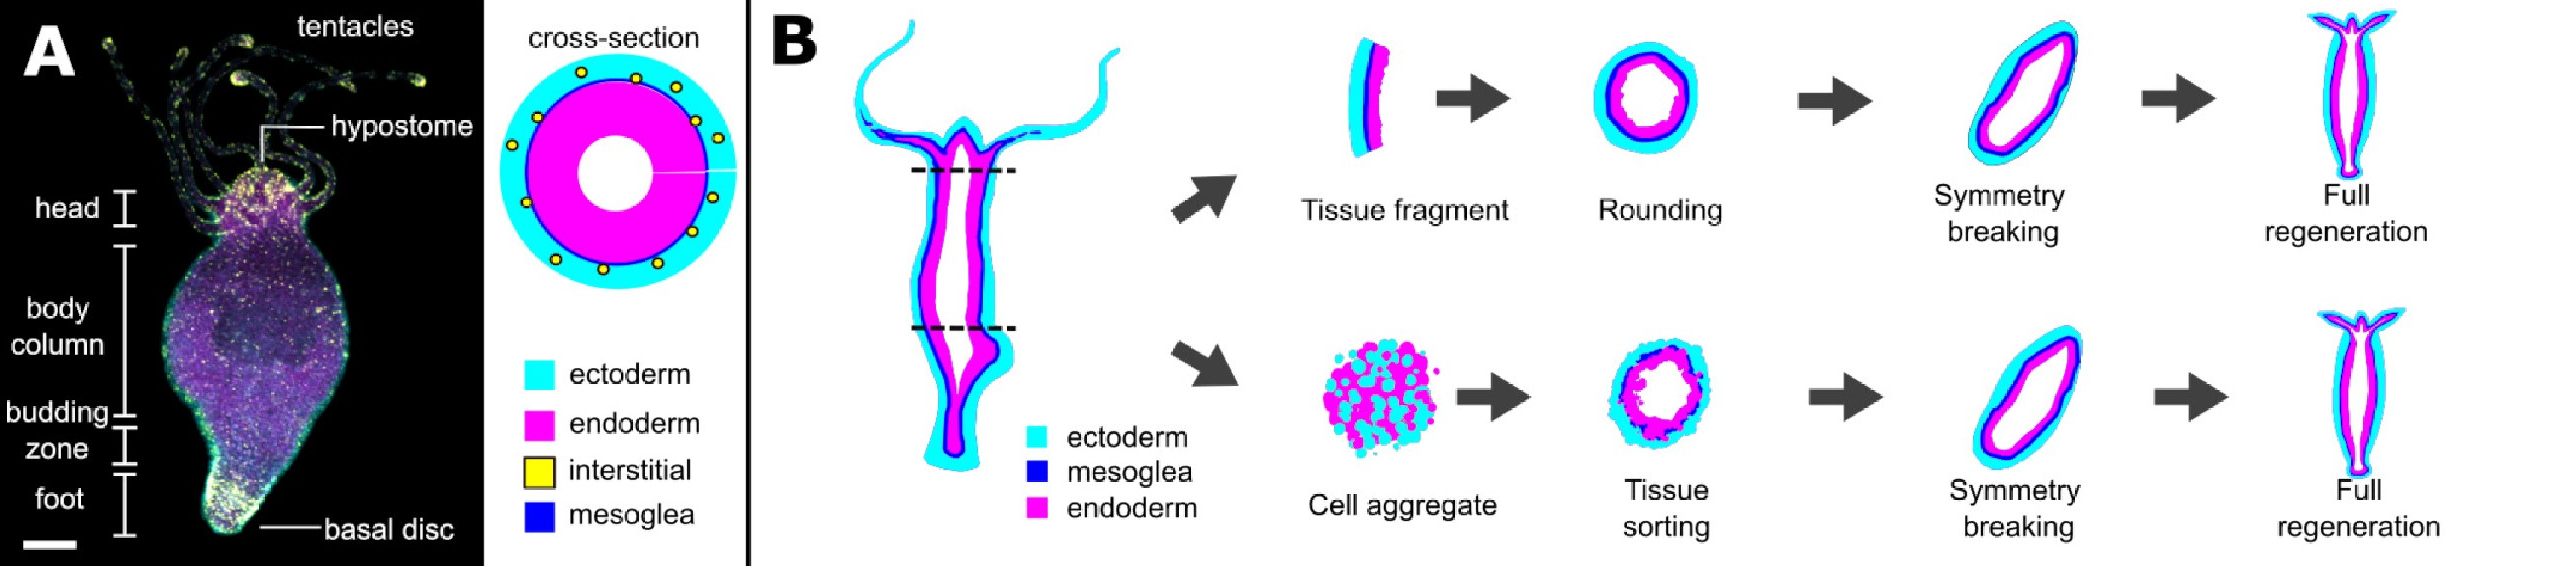
\includegraphics[
        width=\linewidth,
        height=5.20cm,
        keepaspectratio
      ]{figures/mechanochemistry/hydra_biology.png}
    \end{column}

    \begin{column}{0.29\textwidth}
      \HydraPoint[HydraGold]
        {Initially symmetric}
        {A tissue fragment rounds into a hollow spheroid}
      \vspace{-0.08cm}
      \HydraPoint[HydraCyan]
        {Symmetry is broken}
        {One region becomes the future head organizer}
      \vspace{-0.08cm}
      \HydraPoint[HydraGreen]
        {A complete axis emerges}
        {The localized organizer directs whole-body regeneration}
    \end{column}
  \end{columns}

  \source{Wang et al., Integrative and Comparative Biology, 2023}

\end{frame}


\begin{frame}{The central question}

  \vspace{0.40cm}

  \begin{center}
    \begin{minipage}{0.84\linewidth}
      \centering
      {\color{HydraMuted}\fontsize{8.2}{10}\selectfont
        Can a local morphogen change the mechanics of the entire spheroid?
      \par}
      \vspace{0.36cm}
      {\color{HydraWhite}\bfseries\fontsize{18}{23}\selectfont
        Can mechanics replace the diffusible inhibitor?
      \par}
      \vspace{0.46cm}
      {\color{HydraCyan}\fontsize{20}{20}\selectfont $\Downarrow$\par}
      \vspace{0.40cm}
      {\color{HydraGold}\bfseries\fontsize{12}{15}\selectfont
        Build the simplest mechanochemical model that can answer this question
      \par}
    \end{minipage}
  \end{center}

\end{frame}


\HydraSubsection[
  \mbox{Swelling and rupture expose}
  \mbox{a two-way coupling between}
  \mbox{morphogen signaling and mechanics}
]{Mechanics during regeneration}


\begin{frame}{One oscillation is a swelling and rupture cycle}

  \vspace{0.22cm}

  \HydraProcess{water enters}{tissue stretches}{tissue ruptures}

  \vspace{0.54cm}

  \begin{center}
    {\color{HydraCyan}\fontsize{19}{19}\selectfont $\Downarrow$}

    \vspace{0.28cm}

    {\color{HydraGreen}\bfseries\fontsize{12}{15}\selectfont
      the tissue deflates, heals, and the cycle begins again
    \par}
  \end{center}

  \vspace{0.46cm}

  \HydraTakeaway{
    Osmotic pressure repeatedly converts fluid transport into tissue stretching
  }

\end{frame}


\begin{frame}{The spheroid radius records repeated rupture events}

  \vspace{-0.18cm}

  \begin{columns}[c,onlytextwidth]
    \begin{column}{0.72\textwidth}
      \centering
      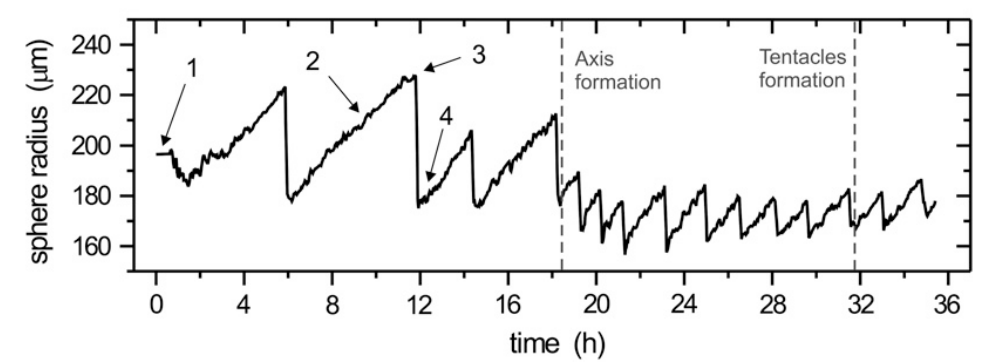
\includegraphics[
        width=\linewidth,
        height=5.25cm,
        keepaspectratio
      ]{figures/mechanochemistry/oscillation_radius.png}
    \end{column}

    \begin{column}{0.24\textwidth}
      \HydraPoint[HydraGold]
        {Slow increase}
        {Water influx gradually increases the spheroid radius}
      \vspace{-0.06cm}
      \HydraPoint[HydraRed]
        {Rapid decrease}
        {Rupture releases fluid and abruptly reduces the radius}
      \vspace{-0.06cm}
      \HydraPoint[HydraCyan]
        {Changing dynamics}
        {The oscillation changes as the body axis and tentacles form}
    \end{column}
  \end{columns}

  \source{Kuecken et al., Biophysical Journal, 2008}

\end{frame}


\begin{frame}{Wnt3 changes the oscillatory dynamics}

  \vspace{-0.18cm}

  \begin{columns}[c,onlytextwidth]
    \begin{column}{0.72\textwidth}
      \centering
      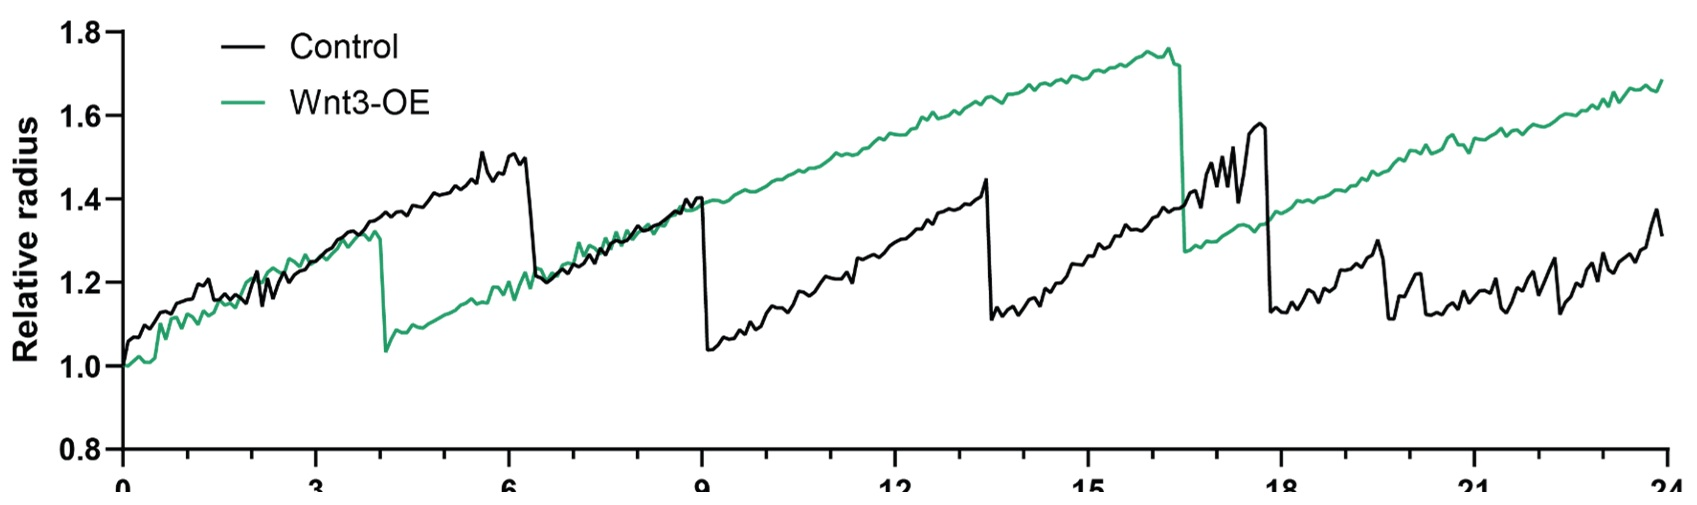
\includegraphics[
        width=\linewidth,
        height=5.15cm,
        keepaspectratio
      ]{figures/mechanochemistry/oscillation_wnt3_oe.jpg}
    \end{column}

    \begin{column}{0.24\textwidth}
      \HydraPoint[HydraGold]
        {Control}
        {Repeated rupture limits the gradual increase in radius}
      \vspace{-0.02cm}
      \HydraPoint[HydraGreen]
        {Wnt3 overexpression}
        {The timing and amplitude of rupture events are altered}
      \vspace{-0.02cm}
      {\color{HydraMuted}\fontsize{7.1}{8.7}\selectfont
        Morphogen signaling and tissue-scale mechanics cannot be treated independently
      \par}
    \end{column}
  \end{columns}

\end{frame}


\begin{frame}{Experiments suggest a mechanochemical coupling}

  \vspace{0.10cm}

  \begin{columns}[c,onlytextwidth]
    \begin{column}{0.44\textwidth}
      \centering
      {\color{HydraGold}\bfseries\fontsize{9.2}{11}\selectfont TISSUE STRETCHING\par}
      \vspace{0.32cm}
      {\color{HydraCyan}\fontsize{19}{19}\selectfont $\Downarrow$}
      \vspace{0.28cm}
      {\color{HydraWhite}\bfseries\fontsize{11.5}{14}\selectfont Wnt3 production\par}
      \vspace{0.24cm}
      {\color{HydraMuted}\fontsize{7.3}{9}\selectfont
        Stretching correlates with organizer formation and Wnt3 expression
      \par}
    \end{column}

    \begin{column}{0.08\textwidth}
      \centering{\color{HydraLine}\fontsize{30}{30}\selectfont $\vert$}
    \end{column}

    \begin{column}{0.44\textwidth}
      \centering
      {\color{HydraWhite}\bfseries\fontsize{11.5}{14}\selectfont MORPHOGEN\par}
      \vspace{0.32cm}
      {\color{HydraCyan}\fontsize{19}{19}\selectfont $\Downarrow$}
      \vspace{0.28cm}
      {\color{HydraGreen}\bfseries\fontsize{10.2}{12.5}\selectfont Tissue elasticity\par}
      \vspace{0.24cm}
      {\color{HydraMuted}\fontsize{7.3}{9}\selectfont
        Morphogen signaling changes how strongly the tissue resists deformation
      \par}
    \end{column}
  \end{columns}

  \vspace{0.52cm}
  \HydraTakeaway{Each side of the feedback modifies the other}

\end{frame}


\begin{frame}{Mechanochemical feedback}

  \vspace{-0.18cm}

  \begin{columns}[c,onlytextwidth]
    \begin{column}{0.62\textwidth}
      \centering
      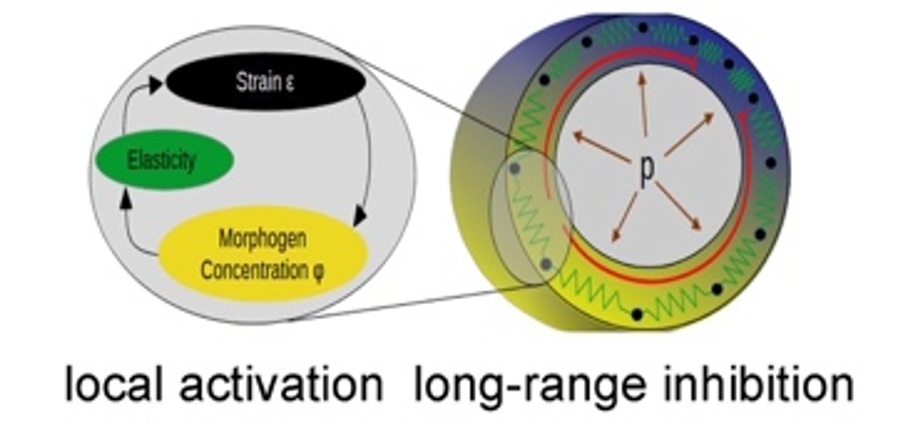
\includegraphics[
        width=\linewidth,
        height=5.35cm,
        keepaspectratio
      ]{figures/mechanochemistry/3d_intersection.jpg}
    \end{column}

    \begin{column}{0.34\textwidth}
      \HydraPoint[HydraGold]
        {Local activation}
        {Morphogen changes elasticity and concentrates strain locally}
      \vspace{-0.05cm}
      \HydraPoint[HydraCyan]
        {Long-range inhibition}
        {The closed pressurized tissue shares a finite total deformation}
      \vspace{-0.05cm}
      \HydraPoint[HydraGold]
        {Minimal ingredients}
        {Morphogen dynamics, mechanics and one global constraint}
    \end{column}
  \end{columns}

\end{frame}

\HydraSubsection[
  \mbox{A closed ring of springs reveals}
  \mbox{how local elasticity produces}
  \mbox{a global redistribution of strain}
]{From springs to a continuum}


% \begin{frame}{Replace the spheroid by an elastic ring}

%   \vspace{-0.18cm}

%   \begin{columns}[c,onlytextwidth]
%     \begin{column}{0.48\textwidth}
%       \centering
%       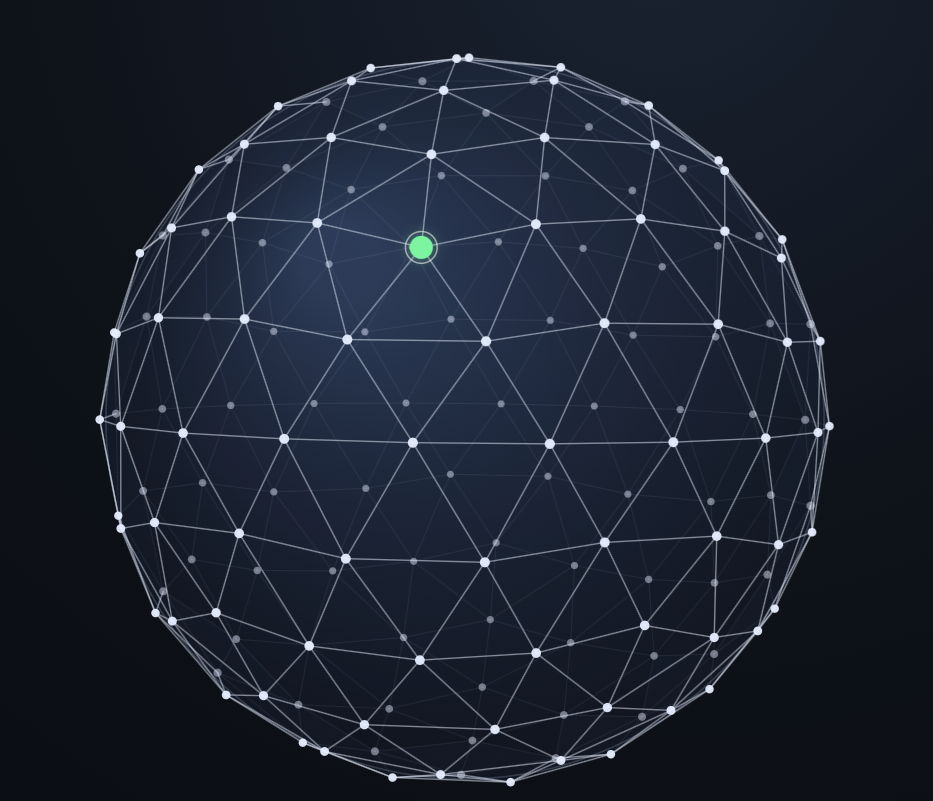
\includegraphics[
%         width=\linewidth,
%         height=4.95cm,
%         keepaspectratio
%       ]{figures/mechanochemistry/sphere_springs.png}
%     \end{column}

%     \begin{column}{0.48\textwidth}
%       \HydraPoint[HydraGold]
%         {Closed geometry}
%         {The one-dimensional ring represents a cross-section of the spheroid}
%       \vspace{-0.04cm}
%       \HydraPoint[HydraCyan]
%         {Elastic tissue}
%         {Neighbouring material points are connected by springs}
%       \vspace{-0.04cm}
%       \HydraPoint[HydraGreen]
%         {Morphogen-dependent stiffness}
%         {Each spring responds to the local concentration of morphogen}
%     \end{column}
%   \end{columns}

%   \HydraTakeaway{
%     The ring retains the essential coupling while removing unnecessary geometry
%   }

% \end{frame}


\begin{frame}{Local changes redistribute strain around the ring}

  \vspace{-0.18cm}

  \begin{columns}[c,onlytextwidth]
    \begin{column}{0.65\textwidth}
      \centering
      \begin{tikzpicture}[x=1cm,y=1cm]
        \fill[HydraPanel] (0.20,0.25) rectangle (9.45,5.05);
        \draw[HydraLine,line width=1.0pt,rounded corners=3pt]
          (0.20,0.25) rectangle (9.45,5.05);
        \foreach \a in {0,30,...,330}{
          \fill[HydraWhite]
            ({4.82+1.72*cos(\a)},{2.65+1.72*sin(\a)}) circle[radius=0.055cm];
        }
        \draw[HydraCyan,line width=1.0pt]
          plot[domain=0:360,samples=13]
            ({4.82+1.72*cos(\x)},{2.65+1.72*sin(\x)});
        \fill[HydraGold] ({4.82+1.72*cos(30)},{2.65+1.72*sin(30)}) circle[radius=0.12cm];
      \end{tikzpicture}
    \end{column}

    \begin{column}{0.31\textwidth}
      \HydraPoint[HydraGold]
        {Move one node}
        {A local displacement changes several neighboring springs}
      \vspace{-0.04cm}
      \HydraPoint[HydraCyan]
        {Change one stiffness}
        {A softer spring takes a larger share of the deformation}
      \vspace{-0.04cm}
      \HydraPoint[HydraGold]
        {Close the ring}
        {The total extension cannot be assigned independently at every point}
    \end{column}
  \end{columns}

\end{frame}


\begin{frame}{A ring contains many small springs}

  \vspace{-0.14cm}

  \begin{columns}[c,onlytextwidth]
    \begin{column}{0.60\textwidth}
      \centering
      \begin{tikzpicture}[x=0.95cm,y=0.95cm]
        \def\R{2.45}
        \coordinate (O) at (3.40,2.75);
        \foreach \a in {0,20,...,340}{
          \fill[HydraWhite] ($(O)+(\a:\R)$) circle[radius=0.060cm];
        }
        \draw[HydraCyan,line width=1.0pt]
          plot[domain=0:360,samples=19]
            ({3.40+\R*cos(\x)},{2.75+\R*sin(\x)});
        \fill[HydraGold] ($(O)+(40:\R)$) circle[radius=0.105cm];
        \fill[HydraGold] ($(O)+(60:\R)$) circle[radius=0.105cm];
        \draw[HydraGold,line width=2.0pt]
          ($(O)+(40:\R)$) -- ($(O)+(60:\R)$);
        \node[anchor=south west,text=HydraGold,
          font=\bfseries\fontsize{7.4}{8.8}\selectfont]
          at ($(O)+(50:2.72)$) {spring $i$};
        \node[text=HydraMuted,font=\fontsize{7}{8.5}\selectfont]
          at (3.40,2.75) {$N$ springs};
      \end{tikzpicture}
    \end{column}

    \begin{column}{0.36\textwidth}
      {\color{HydraWhite}\fontsize{10}{12.6}\selectfont
      \begin{align*}
        \Delta x&=\frac{L}{N}
        \\
        x_i&=i\Delta x
        \\
        i&=0,\ldots,N-1
      \end{align*}
      }
      \par
      \vspace{-0.32cm}
      {\color{HydraMuted}\fontsize{7.5}{9.2}\selectfont
        Every spring represents a short material segment of reference length $\Delta x$
      \par}
    \end{column}
  \end{columns}

\end{frame}


\begin{frame}{Compare the reference and deformed spring}

  \vspace{0.05cm}

  \begin{columns}[c,onlytextwidth]
    \begin{column}{0.46\textwidth}
      \centering
      {\color{HydraGold}\bfseries\fontsize{8}{9.5}\selectfont
        REFERENCE CONFIGURATION\par}
      \vspace{0.30cm}
      \begin{tikzpicture}[x=1cm,y=1cm]
        \fill[HydraWhite] (0.55,2.10) circle[radius=0.095cm];
        \fill[HydraWhite] (5.10,2.10) circle[radius=0.095cm];
        \draw[HydraLine,line width=1.6pt] (0.55,2.10) -- (5.10,2.10);
        \draw[<->,HydraGold,line width=1.0pt] (0.55,1.35) -- (5.10,1.35);
        \node[text=HydraGold,font=\bfseries\fontsize{8}{9.5}\selectfont]
          at (2.82,0.92) {$\Delta x$};
      \end{tikzpicture}
    \end{column}

    \begin{column}{0.06\textwidth}
      \centering{\color{HydraCyan}\fontsize{19}{19}\selectfont $\Rightarrow$}
    \end{column}

    \begin{column}{0.46\textwidth}
      \centering
      {\color{HydraCyan}\bfseries\fontsize{8}{9.5}\selectfont
        DEFORMED CONFIGURATION\par}
      \vspace{0.30cm}
      \begin{tikzpicture}[x=1cm,y=1cm]
        \fill[HydraWhite] (0.30,2.10) circle[radius=0.095cm];
        \fill[HydraWhite] (5.55,2.10) circle[radius=0.095cm];
        \draw[HydraCyan,line width=1.6pt] (0.30,2.10) -- (5.55,2.10);
        \draw[<->,HydraCyan,line width=1.0pt] (0.30,1.35) -- (5.55,1.35);
        \node[text=HydraCyan,font=\bfseries\fontsize{8}{9.5}\selectfont]
          at (2.92,0.92) {$\ell_i$};
      \end{tikzpicture}
    \end{column}
  \end{columns}

  \vspace{0.38cm}

  {\color{HydraWhite}\fontsize{10.5}{13.2}\selectfont
  \begin{align*}
    \text{extension of spring } i
    &: \quad \ell_i-\Delta x
  \end{align*}
  }

\end{frame}


\begin{frame}{Strain measures relative extension}

  \vspace{0.18cm}

  \begin{center}
    \begin{minipage}{0.78\linewidth}
      {\color{HydraMuted}\fontsize{8}{9.8}\selectfont
        Absolute extension depends on the size of the spring
      \par}
      \vspace{-0.16cm}
      {\color{HydraWhite}\bfseries\fontsize{15}{18.5}\selectfont
      \begin{align*}
        \boxed{
          \varepsilon_i
          =
          \frac{\ell_i-\Delta x}{\Delta x}
        }
      \end{align*}
      }
      \par
      \vspace{-0.24cm}
      \HydraPoint[HydraCyan]
        {$\varepsilon_i=0$}
        {The spring keeps its reference length}
      \vspace{-0.12cm}
      \HydraPoint[HydraGold]
        {$\varepsilon_i>0$}
        {The spring is stretched}
      \vspace{-0.12cm}
      \HydraPoint[HydraGold]
        {$\varepsilon_i<0$}
        {The spring is compressed}
    \end{minipage}
  \end{center}

\end{frame}


\begin{frame}{The energy of one spring has the correct continuum scaling}

  \vspace{-0.10cm}

  \begin{columns}[c,onlytextwidth]
    \begin{column}{0.52\textwidth}
      {\color{HydraMuted}\fontsize{7.8}{9.5}\selectfont
        Hooke's law assigns the spring energy
      \par}
      \vspace{-0.18cm}
      {\color{HydraWhite}\fontsize{10.2}{12.9}\selectfont
      \begin{align*}
        \mathcal E_i
        &=
        \frac12k_i(u_i)
        \left(\ell_i-\Delta x\right)^2
        \\
        k_i(u_i)&=\frac{E(u_i)}{\Delta x}
      \end{align*}
      }
      \par
      \vspace{-0.34cm}
      {\color{HydraGold}\bfseries\fontsize{11.2}{14.2}\selectfont
      \begin{align*}
        \boxed{
          \mathcal E_i
          =
          \frac12E(u_i)\varepsilon_i^2\Delta x
        }
      \end{align*}
      }
    \end{column}

    \begin{column}{0.44\textwidth}
      \HydraPoint[HydraGold]
        {Quadratic response}
        {Doubling the extension multiplies the elastic energy by four}
      \vspace{-0.04cm}
      \HydraPoint[HydraCyan]
        {Consistent subdivision}
        {Increasing the number of springs does not change the tissue stiffness}
      \vspace{-0.04cm}
      {\color{HydraMuted}\fontsize{7.2}{8.8}\selectfont
        The factor $\Delta x$ prepares the energy for a Riemann-sum limit
      \par}
    \end{column}
  \end{columns}

\end{frame}


\begin{frame}{Morphogen concentration controls local stiffness}

  \vspace{-0.06cm}

  \begin{columns}[c,onlytextwidth]
    \begin{column}{0.48\textwidth}
      {\color{HydraWhite}\bfseries\fontsize{12.2}{15.4}\selectfont
      \begin{align*}
        E'(u)&<0
      \end{align*}
      }
      \par
      \vspace{-0.26cm}
      \HydraPoint[HydraGold]
        {High morphogen}
        {The elastic modulus is smaller and the tissue is softer}
      \vspace{-0.06cm}
      \HydraPoint[HydraCyan]
        {Low morphogen}
        {The elastic modulus is larger and the tissue is stiffer}
      \vspace{-0.12cm}
      {\color{HydraWhite}\fontsize{10.3}{13}\selectfont
      \begin{align*}
        E(u)&=e^{-\beta u}
        \qquad
        \beta>0
      \end{align*}
      }
    \end{column}

    \begin{column}{0.48\textwidth}
      \centering
      \begin{tikzpicture}[x=0.92cm,y=0.92cm]
        \draw[-{Latex[length=2mm]},HydraMuted,line width=0.7pt]
          (0.45,0.55) -- (5.45,0.55)
          node[below,text=HydraMuted,font=\fontsize{7}{8.2}\selectfont] {$u$};
        \draw[-{Latex[length=2mm]},HydraMuted,line width=0.7pt]
          (0.55,0.45) -- (0.55,5.15)
          node[left,text=HydraMuted,font=\fontsize{7}{8.2}\selectfont] {$E(u)$};
        \draw[HydraGold,line width=1.7pt,domain=0.55:5.10,samples=100]
          plot (\x,{0.60+4.05*exp(-0.58*(\x-0.55))});
        \node[anchor=west,text=HydraGold,
          font=\bfseries\fontsize{7.4}{8.8}\selectfont]
          at (3.25,1.45) {$e^{-\beta u}$};
      \end{tikzpicture}
    \end{column}
  \end{columns}

\end{frame}


\begin{frame}{The local feedback is positive}

  \vspace{0.35cm}

  \begin{columns}[c,onlytextwidth]
    \begin{column}{0.24\textwidth}
      \centering{\color{HydraGold}\bfseries\fontsize{10}{12}\selectfont higher $u$\par}
    \end{column}
    \begin{column}{0.06\textwidth}
      \centering{\color{HydraCyan}\fontsize{17}{17}\selectfont $\Rightarrow$}
    \end{column}
    \begin{column}{0.24\textwidth}
      \centering{\color{HydraWhite}\bfseries\fontsize{10}{12}\selectfont smaller $E(u)$\par}
    \end{column}
    \begin{column}{0.06\textwidth}
      \centering{\color{HydraCyan}\fontsize{17}{17}\selectfont $\Rightarrow$}
    \end{column}
    \begin{column}{0.18\textwidth}
      \centering{\color{HydraCyan}\bfseries\fontsize{10}{12}\selectfont larger strain\par}
    \end{column}
    \begin{column}{0.06\textwidth}
      \centering{\color{HydraCyan}\fontsize{17}{17}\selectfont $\Rightarrow$}
    \end{column}
    \begin{column}{0.16\textwidth}
      \centering{\color{HydraGreen}\bfseries\fontsize{10}{12}\selectfont more $u$\par}
    \end{column}
  \end{columns}

  \vspace{0.70cm}

  \begin{center}
    \begin{minipage}{0.78\linewidth}
      \HydraPoint[HydraGold]
        {Local activation}
        {A small local increase in morphogen makes the same region easier to stretch}
      \vspace{-0.10cm}
      \HydraPoint[HydraCyan]
        {Missing ingredient}
        {We still need to determine how the strain is distributed around the entire ring}
    \end{minipage}
  \end{center}

\end{frame}


\begin{frame}{The total discrete energy is a sum over all springs}

  \vspace{0.10cm}

  \begin{center}
    \begin{minipage}{0.82\linewidth}
      {\color{HydraMuted}\fontsize{8}{9.8}\selectfont
        Every spring contributes its local elastic energy
      \par}
      \vspace{-0.10cm}
      {\color{HydraWhite}\bfseries\fontsize{14.2}{17.8}\selectfont
      \begin{align*}
        \mathcal E_N
        =
        \sum_{i=0}^{N-1}\mathcal E_i=
        \sum_{i=0}^{N-1}
        \frac12E(u_i)\varepsilon_i^2\Delta x
      \end{align*}
      }
      \par
      \vspace{-0.28cm}
      \HydraPoint[HydraGold]
        {Local contribution}
        {Each term depends only on the strain and morphogen at spring $i$}
      \vspace{-0.10cm}
      \HydraPoint[HydraCyan]
        {Global configuration}
        {The total energy depends on how deformation is shared by all springs}
    \end{minipage}
  \end{center}

\end{frame}


\begin{frame}{A material coordinate follows the tissue}

  \vspace{-0.06cm}

  \begin{columns}[c,onlytextwidth]
    \begin{column}{0.58\textwidth}
      \centering
      \begin{tikzpicture}[x=0.96cm,y=0.96cm]
        \draw[HydraLine,line width=1.2pt] (2.05,2.75) circle[radius=1.45cm];
        \draw[HydraCyan,line width=1.2pt] (6.25,2.75) circle[radius=2.05cm];
        \fill[HydraGold] ({2.05+1.45*cos(35)},{2.75+1.45*sin(35)}) circle[radius=0.09cm];
        \fill[HydraGold] ({6.25+2.05*cos(35)},{2.75+2.05*sin(35)}) circle[radius=0.09cm];
        \draw[-{Latex[length=2.5mm]},HydraGold,line width=1.0pt]
          ({2.05+1.55*cos(35)},{2.75+1.55*sin(35)}) .. controls (4.00,4.80) ..
          ({6.25+1.95*cos(35)},{2.75+1.95*sin(35)});
        \node[text=HydraMuted,font=\fontsize{7.2}{8.7}\selectfont]
          at (2.05,0.78) {reference ring $[0,L]$};
        \node[text=HydraCyan,font=\fontsize{7.2}{8.7}\selectfont]
          at (6.25,0.20) {deformed ring $[0,\ell]$};
        \node[text=HydraGold,font=\bfseries\fontsize{7.2}{8.7}\selectfont]
          at (4.20,4.88) {$s(x)$};
      \end{tikzpicture}
    \end{column}

    \begin{column}{0.38\textwidth}
      {\color{HydraWhite}\fontsize{10.6}{13.4}\selectfont
      \begin{align*}
        x&\in[0,L]
        \\
        s(x)&\in[0,\ell]
      \end{align*}
      }
      \par
      \vspace{-0.25cm}
      \HydraPoint[HydraGold]
        {Material label}
        {$x$ identifies a fixed piece of tissue}
      \vspace{-0.06cm}
      \HydraPoint[HydraCyan]
        {Deformed position}
        {$s(x)$ gives its arc-length position after stretching}
    \end{column}
  \end{columns}

\end{frame}


\begin{frame}{Discrete strain converges to a spatial derivative}

  \vspace{0.05cm}

  \begin{center}
    \begin{minipage}{0.86\linewidth}
      {\color{HydraWhite}\fontsize{10.6}{13.4}\selectfont
      \begin{align*}
        \ell_i
        &=s(x_{i+1})-s(x_i)
        \\
        \varepsilon_i
        &=
        \frac{s(x_{i+1})-s(x_i)}{\Delta x}-1
      \end{align*}
      }
      \par
      \vspace{-0.28cm}
      \begin{center}
        {\color{HydraCyan}\fontsize{17}{17}\selectfont
          $\Delta x\longrightarrow0$
          \qquad
          $\Rightarrow$
        }
      \end{center}
      \vspace{-0.04cm}
      {\color{HydraWhite}\bfseries\fontsize{14.5}{18}\selectfont
      \begin{align*}
        \boxed{\varepsilon(x)=\partial_xs(x)-1}
      \end{align*}
      }
      \par
      \vspace{-0.24cm}
      {\color{HydraMuted}\fontsize{7.6}{9.3}\selectfont
        The strain compares the local deformed length with the reference length
      \par}
    \end{minipage}
  \end{center}

\end{frame}


\begin{frame}{The spring sum becomes a continuum energy}

  \vspace{0.14cm}

  \begin{center}
    \begin{minipage}{0.90\linewidth}
      {\color{HydraWhite}\fontsize{11}{13.8}\selectfont
      \begin{align*}
        \mathcal E_N
        &=
        \sum_{i=0}^{N-1}
        \frac12E(u_i)\varepsilon_i^2\Delta x
      \end{align*}
      }
      \par
      \vspace{-0.24cm}
      \begin{center}
        {\color{HydraCyan}\fontsize{18}{18}\selectfont
          $N\longrightarrow\infty$
          \qquad
          $\Downarrow$
        }
      \end{center}
      \vspace{-0.04cm}
      {\color{HydraGold}\bfseries\fontsize{15}{18.5}\selectfont
      \begin{align*}
        \boxed{
          \mathcal E_{\mathrm{el}}[s;u]
          =
          \frac12\int_0^L E(u(x))\varepsilon(x)^2\,dx
        }
      \end{align*}
      }
      \par
      \vspace{-0.22cm}
      {\color{HydraMuted}\fontsize{7.6}{9.3}\selectfont
        The discrete spring model has become a continuum elastic energy
      \par}
    \end{minipage}
  \end{center}

\end{frame}


\begin{frame}{The closed ring imposes a global length constraint}

  \vspace{0.04cm}

  \begin{columns}[c,onlytextwidth]
    \begin{column}{0.53\textwidth}
      {\color{HydraWhite}\fontsize{10.8}{13.6}\selectfont
      \begin{align*}
        \ell-L
        &=
        \sum_{i=0}^{N-1}
        \left(\ell_i-\Delta x\right)
        \\
        &=
        \sum_{i=0}^{N-1}\varepsilon_i\Delta x
      \end{align*}
      }
      \par
      \vspace{-0.26cm}
      \begin{center}{\color{HydraCyan}\fontsize{17}{17}\selectfont $\Downarrow$}\end{center}
      \vspace{-0.08cm}
      {\color{HydraGold}\bfseries\fontsize{13.2}{16.5}\selectfont
      \begin{align*}
        \boxed{\ell-L=\int_0^L\varepsilon(x)\,dx}
      \end{align*}
      }
    \end{column}

    \begin{column}{0.43\textwidth}
      \HydraPoint[HydraGold]
        {Total extension is prescribed}
        {Inflation determines how much longer the deformed ring is}
      \vspace{-0.02cm}
      \HydraPoint[HydraCyan]
        {Local strains are coupled}
        {More extension in one region leaves less extension for the rest of the ring}
    \end{column}
  \end{columns}

\end{frame}


\begin{frame}{Mechanical equilibrium minimizes elastic energy}

  \vspace{0.10cm}

  \begin{center}
    \begin{minipage}{0.84\linewidth}
      {\color{HydraMuted}\fontsize{7.8}{9.5}\selectfont
        Mechanics relaxes rapidly compared with morphogen dynamics
      \par}
      \vspace{-0.10cm}
      {\color{HydraWhite}\bfseries\fontsize{13.2}{16.6}\selectfont
      \begin{align*}
        s
        &\in
        \operatorname*{arg\,min}
        \left\{
          \frac12\int_0^L E(u)\varepsilon^2\,dx
        \right\}
      \end{align*}
      }
      \par
      \vspace{-0.26cm}
      {\color{HydraWhite}\fontsize{10.4}{13.2}\selectfont
      \begin{align*}
        \varepsilon&=\partial_xs-1
        \\
        \int_0^L\varepsilon\,dx&=\ell-L
      \end{align*}
      }
      \par
      \vspace{-0.28cm}
      \HydraPoint[HydraGold]
        {Quasi-static mechanics}
        {For each current morphogen profile the tissue immediately reaches mechanical equilibrium}
    \end{minipage}
  \end{center}

\end{frame}


\begin{frame}{Perturb the deformation to compute the first variation}

  \vspace{0.02cm}

  \begin{columns}[c,onlytextwidth]
    \begin{column}{0.47\textwidth}
      {\color{HydraWhite}\fontsize{10.4}{13.2}\selectfont
      \begin{align*}
        s_\theta(x)&=s(x)+\theta h(x)
        \\
        \varepsilon_\theta&=\partial_xs_\theta-1
        \\
        &=\varepsilon+\theta\partial_xh
      \end{align*}
      }
      \par
      \vspace{-0.30cm}
      {\color{HydraMuted}\fontsize{7.4}{9.1}\selectfont
        The periodic perturbation $h$ preserves the closed geometry
      \par}
    \end{column}

    \begin{column}{0.49\textwidth}
      {\color{HydraWhite}\fontsize{9.6}{12.2}\selectfont
      \begin{align*}
        \mathcal E_{\mathrm{el}}[s_\theta;u]
        &=
        \frac12\int_0^L
        E(u)
        \left(\varepsilon+\theta\partial_xh\right)^2\,dx
      \end{align*}
      }
      \par
      \vspace{-0.26cm}
      {\color{HydraGold}\bfseries\fontsize{10.5}{13.2}\selectfont
      \begin{align*}
        \delta\mathcal E_{\mathrm{el}}
        &=
        \left.\frac{d}{d\theta}
        \mathcal E_{\mathrm{el}}[s_\theta;u]
        \right|_{\theta=0}
        \\
        &=\int_0^L E(u)\varepsilon\partial_xh\,dx
      \end{align*}
      }
    \end{column}
  \end{columns}

\end{frame}


\begin{frame}{Integration by parts gives mechanical equilibrium}

  \vspace{0.12cm}

  \begin{center}
    \begin{minipage}{0.88\linewidth}
      {\color{HydraWhite}\fontsize{10.5}{13.2}\selectfont
      \begin{align*}
        \delta\mathcal E_{\mathrm{el}}
        &=\int_0^L E(u)\varepsilon\partial_xh\,dx
        \\
        &=-\int_0^L
        \partial_x\!\left(E(u)\varepsilon\right)h\,dx
      \end{align*}
      }
      \par
      \vspace{-0.24cm}
      {\color{HydraMuted}\fontsize{7.7}{9.4}\selectfont
        The first variation vanishes for every admissible perturbation $h$
      \par}
      \vspace{-0.14cm}
      {\color{HydraGold}\bfseries\fontsize{15}{18.5}\selectfont
      \begin{align*}
        \boxed{\partial_x\!\left(E(u)\varepsilon\right)=0}
      \end{align*}
      }
    \end{minipage}
  \end{center}

\end{frame}


\begin{frame}{Mechanical equilibrium determines the strain explicitly}

  \vspace{-0.14cm}

  {\color{HydraWhite}\fontsize{9.8}{12.5}\selectfont
  \begin{align*}
    E(u(x,t))\varepsilon(x,t)&=\sigma(t)
    \\
    \varepsilon(x,t)&=\frac{\sigma(t)}{E(u(x,t))}
  \end{align*}
  }
  \par
  \vspace{-0.38cm}
  {\color{HydraWhite}\fontsize{9.4}{12}\selectfont
  \begin{align*}
    \ell-L
    &=\sigma(t)\int_0^L\frac{1}{E(u(y,t))}\,dy
  \end{align*}
  }
  \par
  \vspace{-0.32cm}
  {\color{HydraGold}\bfseries\fontsize{11.5}{14.5}\selectfont
  \begin{align*}
    \boxed{
      \varepsilon(x,t)
      =
      \frac{\ell-L}
      {E(u(x,t))
      \displaystyle\int_0^L\frac{1}{E(u(y,t))}\,dy}
    }
  \end{align*}
  }

\end{frame}


\begin{frame}{The full model couples dynamics and mechanical equilibrium}

  \vspace{-0.12cm}

  \begin{columns}[c,onlytextwidth]
    \begin{column}{0.62\textwidth}
      {\color{HydraWhite}\fontsize{10.6}{13.4}\selectfont
      \begin{align*}
        \partial_tu
        &=D\partial_{xx}u-\alpha u+\kappa\varepsilon
        \\
        0
        &=\partial_x\!\left(E(u)\varepsilon\right)
        \\
        \ell-L
        &=\int_0^L\varepsilon(x,t)\,dx
      \end{align*}
      }
      \par
      \vspace{-0.24cm}
      {\color{HydraMuted}\fontsize{7.5}{9.2}\selectfont
        supplemented with periodic boundary conditions and an initial morphogen profile
      \par}
    \end{column}

    \begin{column}{0.34\textwidth}
      \HydraPoint[HydraGold]
        {One evolution equation}
        {Only the morphogen has its own time dynamics}
      \vspace{-0.04cm}
      \HydraPoint[HydraCyan]
        {Instantaneous mechanics}
        {Strain is determined by equilibrium at every time}
      \vspace{-0.04cm}
      \HydraPoint[HydraGold]
        {One global constraint}
        {The prescribed total extension couples the entire ring}
    \end{column}
  \end{columns}

\end{frame}


\begin{frame}{Mechanical variables can be eliminated exactly}

  \vspace{-0.12cm}

  {\color{HydraWhite}\fontsize{9.0}{11.4}\selectfont
  \begin{align*}
    \partial_tu
    &=D\partial_{xx}u-\alpha u+\kappa\varepsilon
    \\
    \varepsilon(x,t)
    &=
    \frac{\ell-L}
    {E(u(x,t))
    \displaystyle\int_0^L\frac{1}{E(u(y,t))}\,dy}
  \end{align*}
  }
  \par
  \vspace{-0.28cm}
  \begin{center}{\color{HydraCyan}\fontsize{17}{17}\selectfont $\Downarrow$}\end{center}
  \vspace{-0.08cm}
  {\color{HydraGold}\bfseries\fontsize{9.6}{12.2}\selectfont
  \begin{align*}
    \boxed{
      \partial_tu
      =D\partial_{xx}u-\alpha u
      +\kappa
      \frac{\ell-L}
      {E(u(x,t))
      \displaystyle\int_0^L\frac{1}{E(u(y,t))}\,dy}
    }
  \end{align*}
  }

\end{frame}


\begin{frame}{Exponential softening produces the nonlocal feedback}

  \vspace{-0.02cm}

  \begin{columns}[c,onlytextwidth]
    \begin{column}{0.43\textwidth}
      {\color{HydraWhite}\fontsize{10.6}{13.4}\selectfont
      \begin{align*}
        E(u)&=e^{-\beta u}
        \\
        \frac{1}{E(u)}&=e^{\beta u}
      \end{align*}
      }
      \par
      \vspace{-0.30cm}
      \HydraPoint[HydraGold]
        {Local factor}
        {$e^{\beta u(x,t)}$ amplifies regions with larger morphogen}
    \end{column}

    \begin{column}{0.53\textwidth}
      {\color{HydraGold}\bfseries\fontsize{10.8}{13.6}\selectfont
      \begin{align*}
        \varepsilon(x,t)
        &=
        (\ell-L)
        \frac{e^{\beta u(x,t)}}
        {\displaystyle\int_0^L e^{\beta u(y,t)}\,dy}
      \end{align*}
      }
      \par
      \vspace{-0.24cm}
      \HydraPoint[HydraCyan]
        {Global factor}
        {The denominator preserves the prescribed total extension}
    \end{column}
  \end{columns}

  \vspace{0.30cm}
  \HydraTakeaway{
    The mechanics generates a local exponential activation divided by a global normalization
  }

\end{frame}


\begin{frame}{Nondimensionalization gives one nonlocal equation}

  \vspace{-0.16cm}

  \begin{columns}[c,onlytextwidth]
    \begin{column}{0.35\textwidth}
      {\color{HydraMuted}\fontsize{7.4}{9.1}\selectfont
        Natural variables
      \par}
      \vspace{-0.22cm}
      {\color{HydraWhite}\fontsize{8.8}{11.2}\selectfont
      \begin{align*}
        \widetilde x&=\frac{x}{L}
        \\
        \widetilde t&=\alpha t
        \\
        \widetilde u&=\beta u
      \end{align*}
      }
    \end{column}

    \begin{column}{0.61\textwidth}
      {\color{HydraGold}\bfseries\fontsize{11.4}{14.4}\selectfont
      \begin{align*}
        \boxed{
          \partial_tu
          =D\partial_{xx}u-u
          +\kappa
          \frac{e^{u(x,t)}}
          {\displaystyle\int_0^1e^{u(y,t)}\,dy}
        }
      \end{align*}
      }
      \par
      \vspace{-0.26cm}
      {\color{HydraMuted}\fontsize{7.4}{9.1}\selectfont
        The tildes are dropped and the domain is the unit circle $\mathbb{T}=[0,1]$
      \par}
    \end{column}
  \end{columns}

  \vspace{0.30cm}

  {\color{HydraWhite}\fontsize{8.8}{11.2}\selectfont
  \begin{align*}
    u(0,t)&=u(1,t)
    &
    \partial_xu(0,t)&=\partial_xu(1,t)
    &
    u(x,0)&=u_0(x)
  \end{align*}
  }

\end{frame}


\begin{frame}{One equation realizes the activator--inhibitor paradigm}

  \vspace{-0.05cm}

  \begin{columns}[c,onlytextwidth]
    \begin{column}{0.46\textwidth}
      \centering
      {\color{HydraGold}\bfseries\fontsize{8.2}{9.8}\selectfont
        LOCAL ACTIVATION\par}
      \vspace{-0.18cm}
      {\color{HydraWhite}\fontsize{12.2}{15.3}\selectfont
      \begin{align*}
        e^{u(x,t)}
      \end{align*}
      }
      \par
      \vspace{-0.26cm}
      {\color{HydraMuted}\fontsize{7.5}{9.2}\selectfont
        A region with more morphogen becomes softer and receives more strain-driven production
      \par}
    \end{column}

    \begin{column}{0.08\textwidth}
      \centering{\color{HydraLine}\rule{0.6pt}{2.6cm}}
    \end{column}

    \begin{column}{0.46\textwidth}
      \centering
      {\color{HydraCyan}\bfseries\fontsize{8.2}{9.8}\selectfont
        LONG-RANGE INHIBITION\par}
      \vspace{-0.18cm}
      {\color{HydraWhite}\fontsize{12.2}{15.3}\selectfont
      \begin{align*}
        \int_0^1e^{u(y,t)}\,dy
      \end{align*}
      }
      \par
      \vspace{-0.26cm}
      {\color{HydraMuted}\fontsize{7.5}{9.2}\selectfont
        Increased production in one region reduces the share of extension available elsewhere
      \par}
    \end{column}
  \end{columns}

  \vspace{0.54cm}
  \HydraTakeaway{
    Mechanical equilibrium converts a local positive feedback into global competition
  }

\end{frame}


\HydraSubsection[
  \mbox{Variational structure determines}
  \mbox{when patterns exist and which}
  \mbox{stationary profiles can be stable}
]{Steady states and stability}


\begin{frame}{Stationary patterns solve a nonlocal boundary-value problem}

  \vspace{0.02cm}

  \begin{columns}[c,onlytextwidth]
    \begin{column}{0.62\textwidth}
      {\color{HydraWhite}\fontsize{11}{13.9}\selectfont
      \begin{align*}
        0
        &=D\partial_{xx}U-U
        +\kappa
        \frac{e^{U(x)}}
        {\displaystyle\int_0^1e^{U(y)}\,dy}
      \end{align*}
      }
      \par
      \vspace{-0.20cm}
      {\color{HydraWhite}\fontsize{9.8}{12.5}\selectfont
      \begin{align*}
        U(0)&=U(1)
        \\
        \partial_xU(0)&=\partial_xU(1)
      \end{align*}
      }
    \end{column}

    \begin{column}{0.34\textwidth}
      \HydraPoint[HydraGold]
        {Homogeneous solution}
        {$\bar U\equiv\kappa$ is always a stationary solution}
      \vspace{-0.04cm}
      \HydraPoint[HydraCyan]
        {Patterned solution}
        {A nonconstant periodic function $U(x)$ represents a spatial pattern}
    \end{column}
  \end{columns}

  \vspace{0.18cm}

  {\color{HydraMuted}\fontsize{7.4}{9.1}\selectfont
    Every stationary solution has mean value $\int_0^1U(x)\,dx=\kappa$
  \par}

\end{frame}


\begin{frame}{Small diffusion permits patterns while large diffusion suppresses them}

  \vspace{-0.16cm}

  {\color{HydraGold}\bfseries\fontsize{8.2}{9.8}\selectfont
    THEOREM\par}

  \vspace{0.12cm}

  {\color{HydraWhite}\fontsize{8.5}{10.7}\selectfont
    For every $\kappa>0$ there exist constants
  \par}

  \vspace{-0.34cm}

  {\color{HydraWhite}\bfseries\fontsize{11.2}{14.2}\selectfont
  \begin{align*}
    0<D_{\min}(\kappa)<D_{\max}(\kappa)
  \end{align*}
  }

  \vspace{-0.36cm}

  \begin{columns}[T,onlytextwidth]
    \begin{column}{0.48\textwidth}
      \HydraPoint[HydraGold]
        {$0<D<D_{\min}(\kappa)$}
        {A nonconstant stationary solution exists and is Lyapunov stable in $L^2$}
    \end{column}

    \begin{column}{0.48\textwidth}
      \HydraPoint[HydraCyan]
        {$D>D_{\max}(\kappa)$}
        {$\bar U\equiv\kappa$ is the unique stationary solution and is globally asymptotically stable}
    \end{column}
  \end{columns}

  \vspace{0.20cm}

  {\color{HydraMuted}\fontsize{7.4}{9.1}\selectfont
    The analytic thresholds are sufficient bounds and need not be optimal
  \par}

\end{frame}


\begin{frame}{The parameter plane separates homogeneous and patterned regimes}

  \vspace{-0.16cm}

  \begin{columns}[c,onlytextwidth]
    \begin{column}{0.74\textwidth}
      \centering
      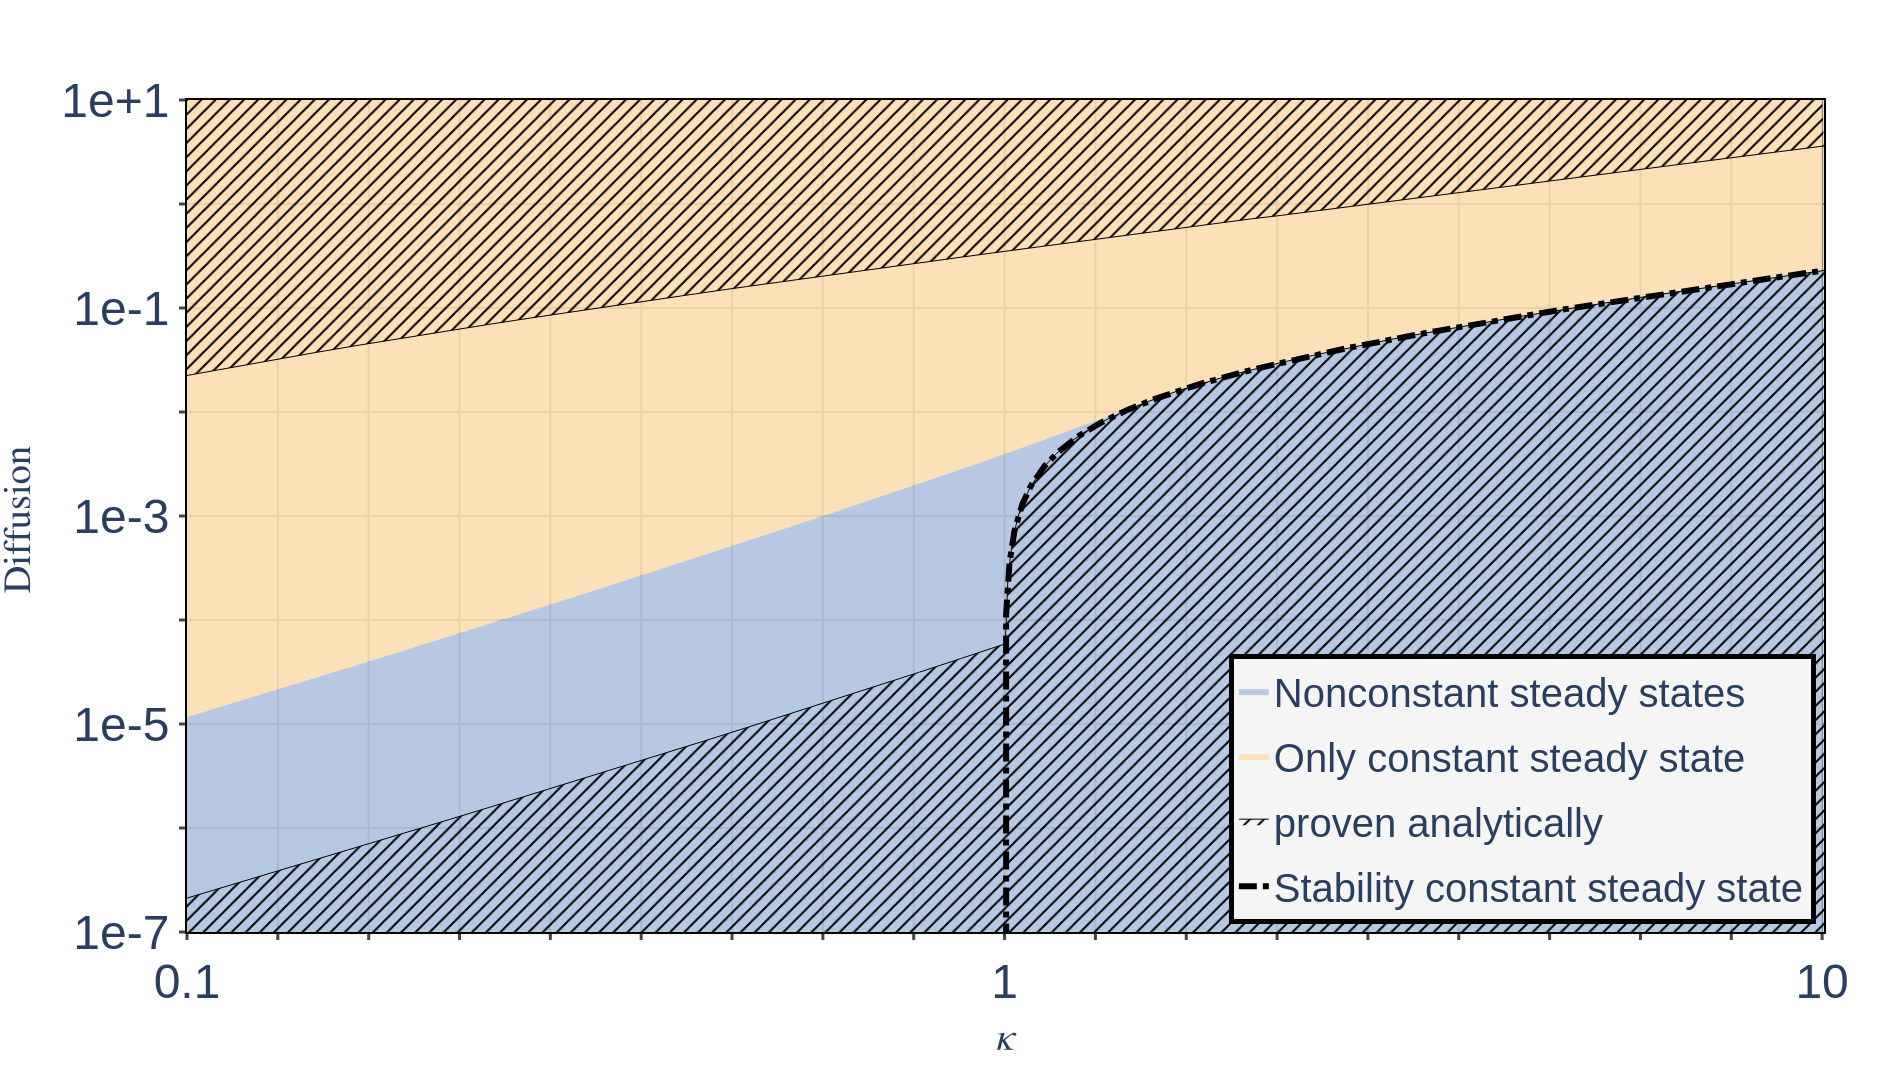
\includegraphics[
        width=\linewidth,
        height=5.35cm,
        keepaspectratio
      ]{figures/mechanochemistry/parameter_space.png}
    \end{column}

    \begin{column}{0.22\textwidth}
      \HydraPoint[HydraCyan]
        {Patterns}
        {Nonconstant steady states are found for sufficiently small diffusion}
      \vspace{-0.10cm}
      \HydraPoint[HydraGold]
        {Homogeneous state}
        {Large diffusion removes spatial variation}
      \vspace{-0.10cm}
      {\color{HydraMuted}\fontsize{6.9}{8.5}\selectfont
        Hatched regions are established analytically
      \par}
    \end{column}
  \end{columns}

\end{frame}


\begin{frame}{Linearization asks whether a stationary profile amplifies perturbations}

  \vspace{-0.10cm}

  {\color{HydraWhite}\fontsize{9.8}{12.4}\selectfont
  \begin{align*}
    u(x,t)&=U(x)+e^{\nu t}\varphi(x)
  \end{align*}
  }

  \vspace{-0.36cm}

  {\color{HydraMuted}\fontsize{7.6}{9.3}\selectfont
    Keeping only first-order terms gives the nonlocal eigenvalue problem
  \par}

  \vspace{-0.24cm}

  {\color{HydraWhite}\fontsize{8.7}{11}\selectfont
  \begin{align*}
    D\partial_{xx}\varphi
    +\left(
      \kappa\frac{e^U}{\int_0^1e^U}-1-\nu
    \right)\varphi
    &=
    \kappa
    \frac{e^U}{\left(\int_0^1e^U\right)^2}
    \int_0^1e^U\varphi
  \end{align*}
  }

  \vspace{-0.24cm}

  \begin{columns}[T,onlytextwidth]
    \begin{column}{0.48\textwidth}
      \HydraPoint[HydraCyan]
        {$\nu<0$}
        {The corresponding perturbation decays}
    \end{column}
    \begin{column}{0.48\textwidth}
      \HydraPoint[HydraGold]
        {$\nu>0$}
        {The corresponding perturbation grows}
    \end{column}
  \end{columns}

\end{frame}


\begin{frame}{A local problem helps locate the nonlocal eigenvalues}

  \vspace{-0.08cm}

  \begin{columns}[c,onlytextwidth]
    \begin{column}{0.48\textwidth}
      \centering
      {\color{HydraGold}\bfseries\fontsize{7.8}{9.4}\selectfont
        NONLOCAL PROBLEM\par}
      \vspace{-0.24cm}
      {\color{HydraWhite}\fontsize{8.7}{11}\selectfont
      \begin{align*}
        D\partial_{xx}\varphi
        +(A-\nu)\varphi
        &=MC(x)\int_0^1C(y)\varphi(y)\,dy
      \end{align*}
      }
      \par
      \vspace{-0.28cm}
      {\color{HydraMuted}\fontsize{7.2}{8.8}\selectfont
        Every value of $\varphi$ is coupled through the integral
      \par}
    \end{column}

    \begin{column}{0.48\textwidth}
      \centering
      {\color{HydraCyan}\bfseries\fontsize{7.8}{9.4}\selectfont
        LOCAL PROBLEM\par}
      \vspace{-0.24cm}
      {\color{HydraWhite}\fontsize{8.7}{11}\selectfont
      \begin{align*}
        D\partial_{xx}\psi
        +(A-\lambda)\psi
        &=0
      \end{align*}
      }
      \par
      \vspace{-0.28cm}
      {\color{HydraMuted}\fontsize{7.2}{8.8}\selectfont
        Classical oscillation theory orders the eigenfunctions by their zeros
      \par}
    \end{column}
  \end{columns}

  \vspace{0.36cm}

  \HydraTakeaway{
    Relevant nonlocal eigenvalues lie between eigenvalues of the associated local problem
  }

\end{frame}


\begin{frame}{Stable mechanochemical patterns are necessarily unimodal}

  \vspace{-0.16cm}

  \begin{columns}[c,onlytextwidth]
    \begin{column}{0.52\textwidth}
      \centering
      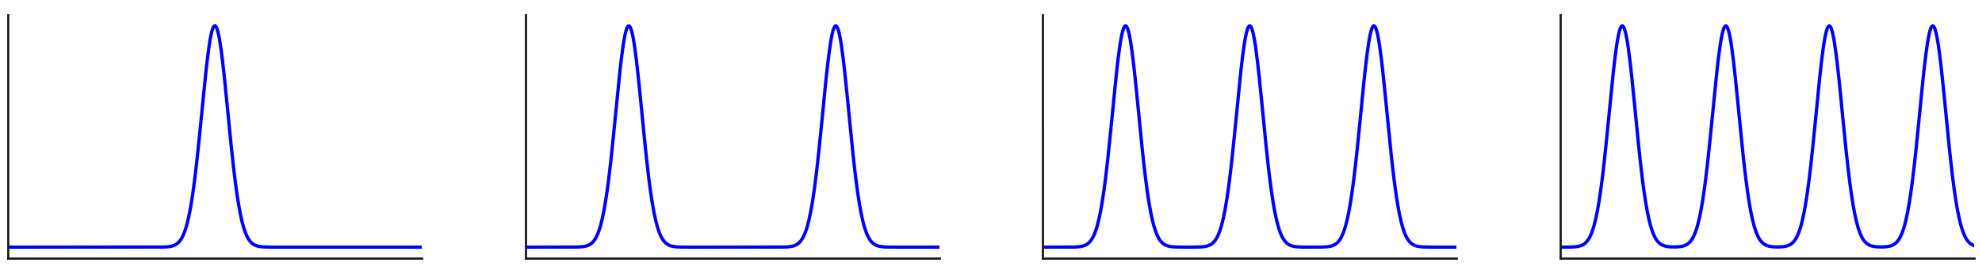
\includegraphics[
        width=\linewidth,
        height=4.65cm,
        keepaspectratio
      ]{figures/mechanochemistry/one_two_peaks.png}
    \end{column}

    \begin{column}{0.44\textwidth}
      {\color{HydraGold}\bfseries\fontsize{8.2}{9.8}\selectfont
        THEOREM\par}
      \vspace{0.16cm}
      \HydraPoint[HydraGreen]
        {Stable nonconstant solution}
        {The stable solution obtained by energy minimization has one peak}
      \vspace{-0.06cm}
      \HydraPoint[HydraRed]
        {Every multimodal solution}
        {All solutions with two or more peaks are linearly and nonlinearly unstable}
      \vspace{-0.06cm}
      {\color{HydraMuted}\fontsize{7.2}{8.8}\selectfont
        The global mechanical constraint strongly selects a single organizer
      \par}
    \end{column}
  \end{columns}

\end{frame}


\begin{frame}{Diffusion changes the width but not the number of stable peaks}

  \vspace{-0.14cm}

  \begin{columns}[c,onlytextwidth]
    \begin{column}{0.72\textwidth}
      \centering
      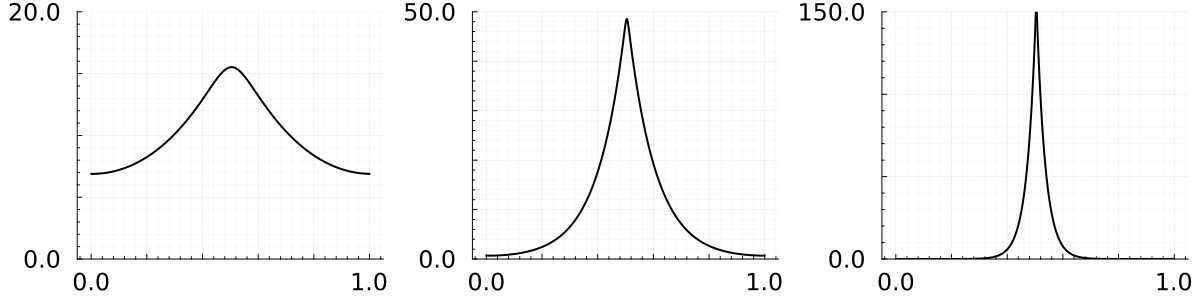
\includegraphics[
        width=\linewidth,
        height=5.15cm,
        keepaspectratio
      ]{figures/mechanochemistry/stationary_profiles.png}
    \end{column}

    \begin{column}{0.24\textwidth}
      \HydraPoint[HydraGold]
        {Smaller diffusion}
        {The stable peak becomes sharper and more localized}
      \vspace{-0.04cm}
      \HydraPoint[HydraCyan]
        {Larger diffusion}
        {The stable profile becomes broader}
      \vspace{-0.04cm}
      \HydraPoint[HydraGreen]
        {Robust selection}
        {The stable pattern retains a single dominant peak}
    \end{column}
  \end{columns}

\end{frame}


\HydraSubsection[
  \mbox{Stationary branches emerge when} \mbox{a homogeneous state changes stability} \mbox{and can generate tissue oscillations}
]{Bifurcations and oscillations}


\begin{frame}{A bifurcation marks a qualitative change in stationary states}

  \vspace{-0.16cm}

  \begin{columns}[c,onlytextwidth]
    \begin{column}{0.57\textwidth}
      \centering
      \begin{tikzpicture}[x=0.88cm,y=0.90cm]
        \draw[-{Latex[length=2.2mm]},HydraMuted,line width=0.75pt]
          (0.45,2.60) -- (7.75,2.60)
          node[anchor=north east,text=HydraMuted,font=\fontsize{7}{8.2}\selectfont] {control parameter $\kappa$};
        \draw[-{Latex[length=2.2mm]},HydraMuted,line width=0.75pt]
          (0.70,0.35) -- (0.70,5.35)
          node[left,text=HydraMuted,font=\fontsize{7}{8.2}\selectfont] {pattern amplitude};

        \draw[HydraCyan,line width=1.65pt]
          (0.75,2.60) -- (7.25,2.60);
        \draw[HydraGold,line width=1.75pt,domain=4.20:7.15,samples=80]
          plot (\x,{2.60+0.78*sqrt(\x-4.20)});
        \draw[HydraGold,line width=1.75pt,domain=4.20:7.15,samples=80]
          plot (\x,{2.60-0.78*sqrt(\x-4.20)});

        \draw[dashed,HydraLine,line width=0.8pt]
          (4.20,0.55) -- (4.20,4.95);
        \fill[HydraWhite] (4.20,2.60) circle[radius=0.085cm];

        \node[anchor=south,text=HydraWhite,
          font=\bfseries\fontsize{7.4}{8.9}\selectfont]
          at (4.20,5.02) {bifurcation point};
        \node[anchor=south west,text=HydraCyan,
          font=\fontsize{7.2}{8.7}\selectfont]
          at (1.20,2.72) {homogeneous state};
        \node[anchor=south west,text=HydraGold,
          font=\fontsize{7.2}{8.7}\selectfont]
          at (5.45,4.25) {patterned states};
      \end{tikzpicture}
    \end{column}

    \begin{column}{0.39\textwidth}
      \HydraPoint[HydraCyan]
        {Before the threshold}
        {Only the homogeneous stationary state is visible nearby}
      \vspace{0.02cm}
      \HydraPoint[HydraGold]
        {At the threshold}
        {A spatial mode becomes neutral and a patterned branch can emerge}
      \vspace{0.02cm}
      \HydraPoint[HydraGold]
        {After the threshold}
        {The number or stability of stationary states has changed}
    \end{column}
  \end{columns}

\end{frame}


\begin{frame}{The homogeneous state loses stability at discrete thresholds}

  \vspace{-0.22cm}

  {\color{HydraWhite}\fontsize{9.6}{12.1}\selectfont
  \begin{align*}
    \bar U&\equiv\kappa
    &
    \varphi_n(x)&=\cos(2\pi n x)
  \end{align*}
  }

  \vspace{-0.44cm}

  {\color{HydraMuted}\fontsize{7.6}{9.3}\selectfont
    Linearization assigns one growth rate to every spatial mode
  \par}

  \vspace{-0.26cm}

  {\color{HydraWhite}\fontsize{10.6}{13.4}\selectfont
  \begin{align*}
    \nu_n&=\kappa-1-4\pi^2n^2D
  \end{align*}
  }

  \vspace{-0.42cm}

  {\color{HydraGold}\bfseries\fontsize{11.2}{14.2}\selectfont
  \begin{align*}
    \boxed{\kappa_n=1+4\pi^2n^2D}
  \end{align*}
  }

  \vspace{-0.34cm}

  \begin{columns}[T,onlytextwidth]
    \begin{column}{0.31\textwidth}
      \HydraPoint[HydraGold]
        {$n=1$}
        {The first nonconstant mode has one maximum and one minimum}
    \end{column}
    \begin{column}{0.31\textwidth}
      \HydraPoint[HydraGold]
        {$n=2$}
        {The next mode produces a two-peak spatial structure}
    \end{column}
    \begin{column}{0.31\textwidth}
      \HydraPoint[HydraCyan]
        {Discrete thresholds}
        {Each mode changes stability at its own value of $\kappa$}
    \end{column}
  \end{columns}

\end{frame}


\begin{frame}{The first patterned branch can be subcritical or supercritical}

  \vspace{-0.12cm}

  {\color{HydraGold}\bfseries\fontsize{8.2}{9.8}\selectfont
    THEOREM\par}

  \vspace{0.20cm}

  {\color{HydraWhite}\fontsize{8.8}{11.1}\selectfont
    At $\kappa=\kappa_n$ a branch of nonconstant stationary solutions bifurcates from the homogeneous state $\bar U\equiv\kappa$
  \par}

  \vspace{0.24cm}

  \begin{columns}[T,onlytextwidth]
    \begin{column}{0.47\textwidth}
      \HydraPoint[HydraGold]
        {Subcritical branch}
        {$\kappa_n<3/2$ equivalently $D<(8\pi^2n^2)^{-1}$}
    \end{column}
    \begin{column}{0.47\textwidth}
      \HydraPoint[HydraCyan]
        {Supercritical branch}
        {$\kappa_n>3/2$ equivalently $D>(8\pi^2n^2)^{-1}$}
    \end{column}
  \end{columns}

  \vspace{0.32cm}

  {\color{HydraMuted}\fontsize{7.6}{9.3}\selectfont
    Near the bifurcation only the supercritical branch generated by the first mode can be stable
  \par}

  \vspace{0.16cm}

  \HydraTakeaway{
    The direction of the branch determines whether small patterned states appear before or after the linear threshold
  }

\end{frame}


\begin{frame}{Diffusion determines the type of each bifurcation}

  \vspace{-0.14cm}

  \begin{columns}[c,onlytextwidth]
    \begin{column}{0.73\textwidth}
      \centering
      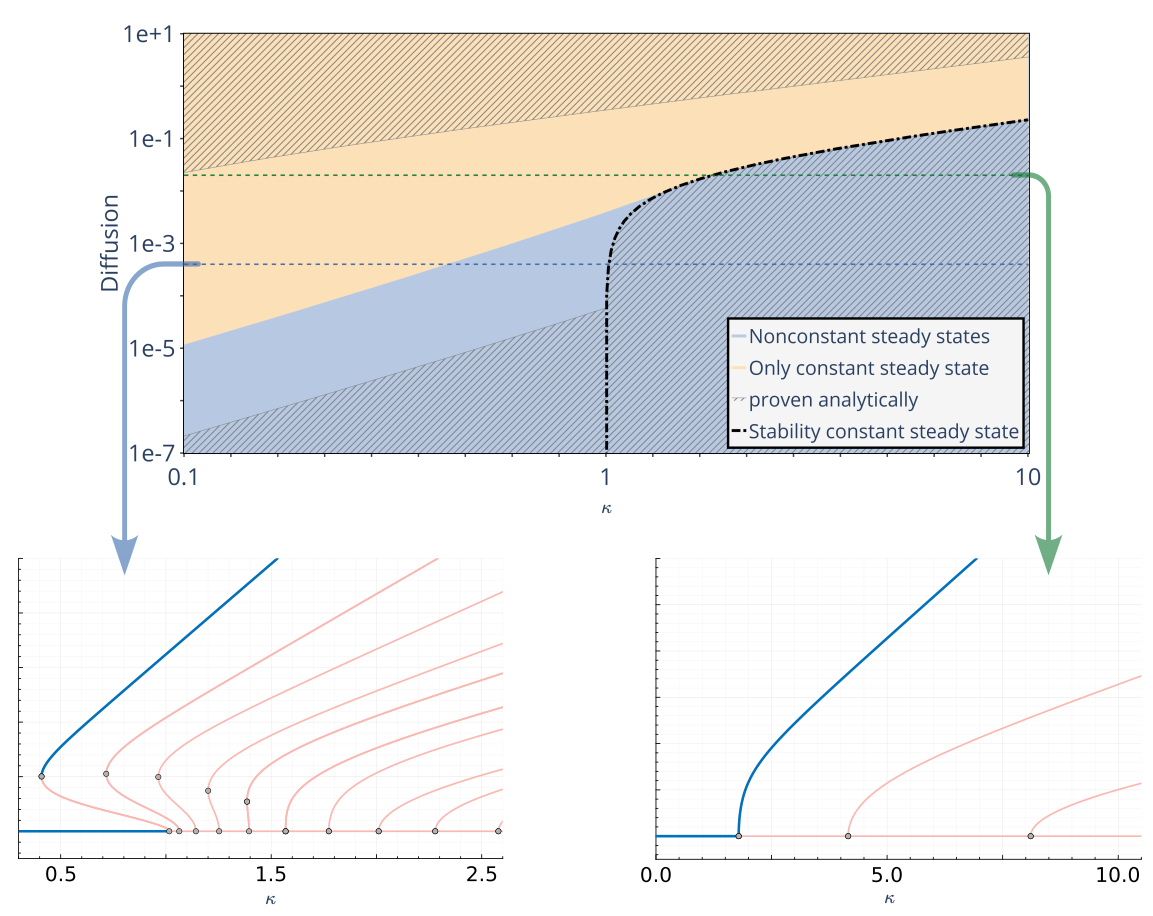
\includegraphics[
        width=\linewidth,
        height=5.25cm,
        keepaspectratio
      ]{figures/mechanochemistry/bifurcation_parameter_map.png}
    \end{column}

    \begin{column}{0.23\textwidth}
      \HydraPoint[HydraGold]
        {Small diffusion}
        {The branch can bend toward smaller values of $\kappa$}
      \vspace{0.04cm}
      \HydraPoint[HydraCyan]
        {Larger diffusion}
        {The branch can emerge toward larger values of $\kappa$}
      \vspace{0.04cm}
      {\color{HydraMuted}\fontsize{7.0}{8.6}\selectfont
        Each spatial mode has its own transition curve
      \par}
    \end{column}
  \end{columns}

\end{frame}


\begin{frame}{Tissue length turns the stationary picture into dynamics}

  \vspace{-0.18cm}

  {\color{HydraMuted}\fontsize{7.6}{9.3}\selectfont
    Let $\ell(t)$ denote the current circumference and $L$ its reference value
  \par}

  \vspace{-0.22cm}

  {\color{HydraWhite}\bfseries\fontsize{10.2}{12.9}\selectfont
  \begin{align*}
    \boxed{
      \partial_tu
      =
      D\partial_{xx}u-u
      +\kappa\bigl(\ell(t)-L\bigr)
      \frac{e^{u(x,t)}}{\int_0^1e^{u(y,t)}\,dy}
    }
  \end{align*}
  }

  \vspace{-0.34cm}

  \begin{columns}[T,onlytextwidth]
    \begin{column}{0.31\textwidth}
      \HydraPoint[HydraGold]
        {Morphogen rises}
        {The tissue softens and the mechanical equilibrium shifts}
    \end{column}
    \begin{column}{0.31\textwidth}
      \HydraPoint[HydraCyan]
        {The spheroid expands}
        {Increased strain strengthens morphogen production}
    \end{column}
    \begin{column}{0.31\textwidth}
      \HydraPoint[HydraGold]
        {Feedback relaxes}
        {Degradation and mechanical restoration can reverse the expansion}
    \end{column}
  \end{columns}

  \vspace{0.18cm}

  \HydraTakeaway{
    Coupling pattern formation to tissue size creates a route from static symmetry breaking to oscillations
  }

\end{frame}


\begin{frame}{Subcritical feedback permits abrupt switching}

  \vspace{-0.12cm}

  \begin{columns}[c,onlytextwidth]
    \begin{column}{0.62\textwidth}
      \centering
      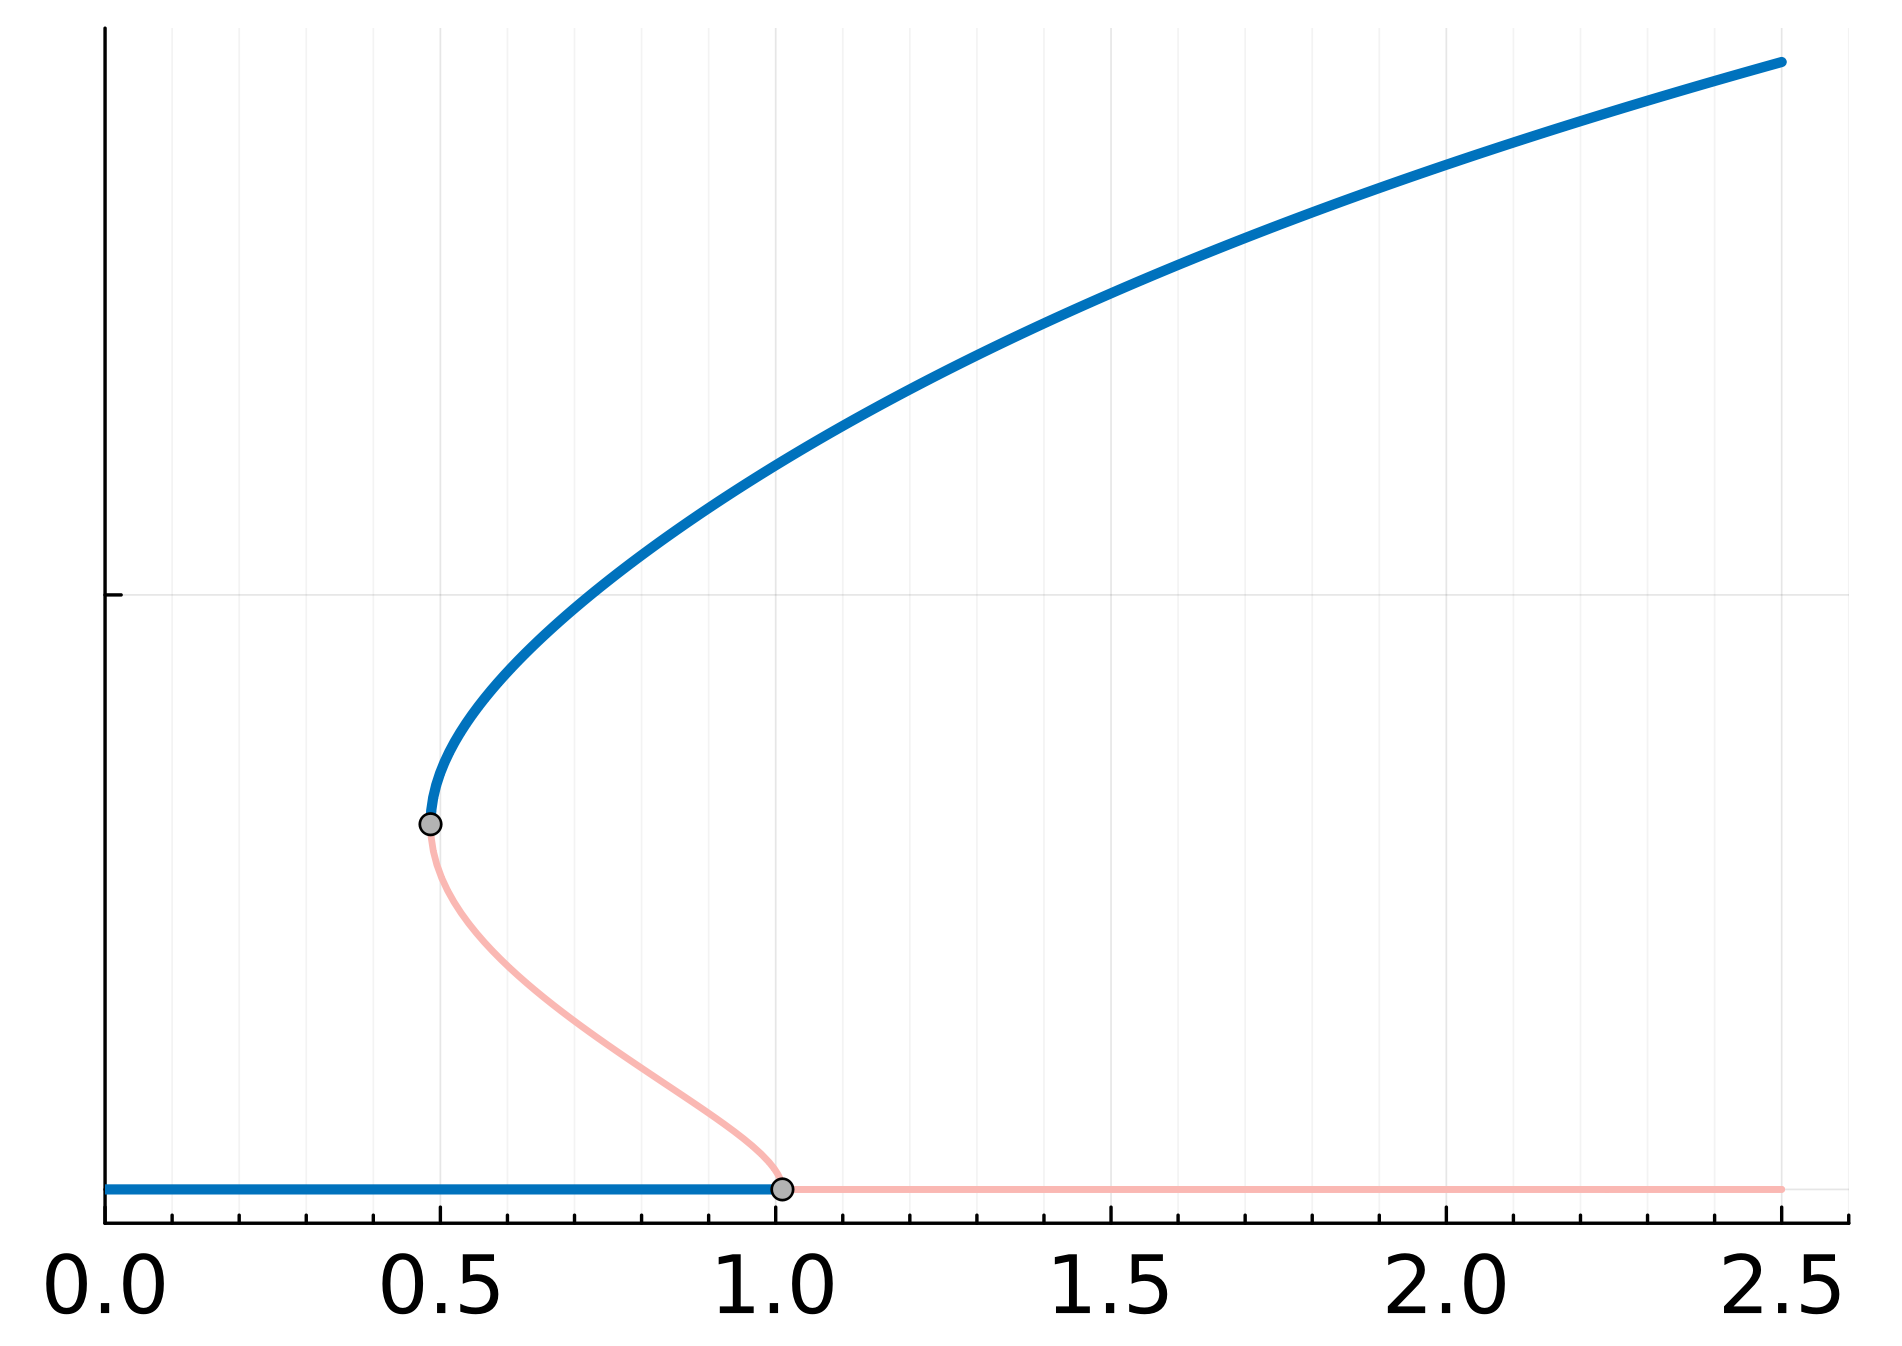
\includegraphics[
        width=\linewidth,
        height=5.05cm,
        keepaspectratio
      ]{figures/mechanochemistry/subcritical_bifurcation.png}
    \end{column}

    \begin{column}{0.34\textwidth}
      \HydraPoint[HydraGold]
        {Coexisting states}
        {A homogeneous and a patterned state may be available for the same parameter value}
      \vspace{0.04cm}
      \HydraPoint[HydraRed]
        {Sudden transition}
        {Crossing a fold can force the system to jump to a distant branch}
    \end{column}
  \end{columns}

\end{frame}


\begin{frame}{Supercritical feedback produces a gradual patterned response}

  \vspace{-0.12cm}

  \begin{columns}[c,onlytextwidth]
    \begin{column}{0.62\textwidth}
      \centering
      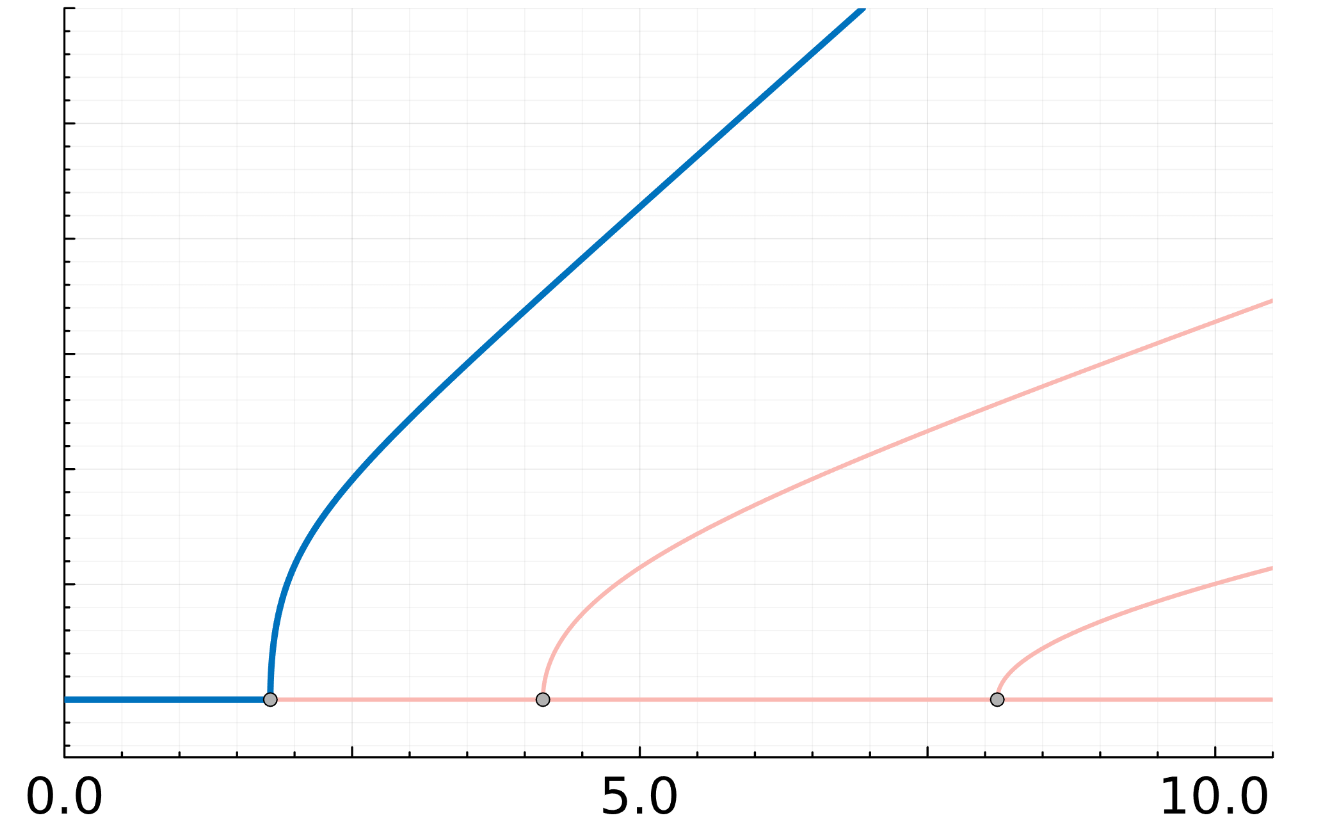
\includegraphics[
        width=\linewidth,
        height=5.05cm,
        keepaspectratio
      ]{figures/mechanochemistry/supercritical_bifurcation.png}
    \end{column}

    \begin{column}{0.34\textwidth}
      \HydraPoint[HydraCyan]
        {Continuous onset}
        {The patterned amplitude grows continuously from the homogeneous state}
      \vspace{0.04cm}
      \HydraPoint[HydraGold]
        {Smooth mechanical response}
        {Tissue deformation can track the changing stationary branch}
    \end{column}
  \end{columns}

\end{frame}


\begin{frame}{Mechanics can realize an activator--inhibitor mechanism without a chemical inhibitor}

  \vspace{-0.08cm}

  \begin{columns}[T,onlytextwidth]
    \begin{column}{0.31\textwidth}
      \HydraPoint[HydraGold]
        {Local positive feedback}
        {Stretch increases morphogen production and morphogen softens the tissue}
    \end{column}
    \begin{column}{0.31\textwidth}
      \HydraPoint[HydraCyan]
        {Global mechanical competition}
        {The fixed total length couples every point through one nonlocal constraint}
    \end{column}
    \begin{column}{0.31\textwidth}
      \HydraPoint[HydraGreen]
        {Single organizer}
        {Stable nonconstant stationary states contain one dominant peak}
    \end{column}
  \end{columns}

  \vspace{0.42cm}

  {\color{HydraWhite}\bfseries\fontsize{12.2}{15.2}\selectfont
  \begin{align*}
    \text{morphogen}
    \quad\Longrightarrow\quad
    \text{softening}
    \quad\Longrightarrow\quad
    \text{strain}
    \quad\Longrightarrow\quad
    \text{morphogen}
  \end{align*}
  }

  \vspace{-0.14cm}

  \HydraTakeaway{
    A single morphogen equation coupled to mechanics can implement local activation and long-range inhibition
  }

\end{frame}


\end{document}
